\chapter{Checks and Systematics}

\section{Summary of Systematic Uncertainties}
The source of systematic uncertainties of the \gammaiso--hadron measurement are the following:
\begin{itemize}
    \item Purity\\
The uncertainty of the purity measurement, is propagated to the correlation function measurement following Equation~\ref{eq:FinalSubtraction}. The resulting uncertainty on the correlation function is a relative $\pm18\%$ for pp data and  $\pm12\%$ for \pPb~data . As described in Section~\ref{sec:puritysystematics}, a large fraction of the purity total uncertainty is either statistical uncertainty or systematic uncertainties that arise due to limited data sample. Therefore, the purity uncertainty in pp and \pPb~data are largely uncorrelated. As a conservative approach, they are taken to be totally uncorrelated.

\item	Underlying Event:\\
As described in Section~\ref{sec:UEsubtraction}, the uncertainty of the UE subtraction originates from statistical fluctuations in the ZYAM estimate. It propagates directly to the per-trigger yields. It ranges from 7\% to 15\% depending on the \zt~bin and data. This uncertainty is fully correlated in $\varphi$ for a given \zt~bin, but totally uncorrelated among \zt~bins, and totally uncorrelated between pp and \pPb~datasets.

\item Tracking performance :\\
To estimate the systematic uncertainty of the charged-particle $\pt$ measurement with ITS-only track reconstruction, MC simulation studies were performed compared with the published \pt~spectra that used the ALICE standard tracking (i.e. including TPC) in pp and \pPb~collisions at 5 TeV~\cite{Acharya:2018qsh}. As described in Section~\ref{sec:tracking}, the combined uncertainty due to track efficiency, fake rate, and bin-to-bin migration corrections amounts to $\pm5\%$ added in quadrature with the total systematic uncertainty of the reference $\pt$ spectra, which ranges from a relative 1.6 (2.1$\%$) to 1.9$\%$ (2.5$\%$) in the range $0.5<\pt<10$ \GeVc~for pp (\pPb) collisions~\cite{Acharya:2018qsh}. 

Systematic uncertainties due to secondary-particle contamination and from modelling of the particle-type composition in MC simulations are small ($<2\%$) for the range $0.5<\pt<10$ \GeVc. These were already estimated in Ref.\cite{Acharya:2018qsh} for pp and \pPb~data sets and already included in the systematic uncertainty estimate described above. The tracking performance between pp and \pPb~datasets is very similar, but as a conservative approach the systematic uncertainties are taken to be completely uncorrelated.


\item Acceptance mismatch due to boost:\\
As described in Section~\ref{sec:bootstudy}, our \textsc{Pythia8} study of \gammaiso--hadron correlations show that the impact of an acceptance mismatch between pp and \pPb~data that arises from the boost of $\Delta y = 0.47$ amounts to about $5\%$ effect irrespective of $\zt$. This estimate is subject to PDF uncertainties, which are the ones that dictate the shape of the differential cross-section of photons and associated hadrons in pseudorapidity. We chose to not apply any correction for this effect, and assign a $\pm$5$\%$ systematic uncertainty on the per-trigger hadron yields. This systematic uncertainty is taken to be completely correlated with \zt. We assign this systematic uncertainty to our \pPb~measurements only. 


\item Luminosity, trigger, photon, and vertex reconstruction:\\
The observable is normalized per measured photon. Therefore the uncertainties related to overall normalization of the \gammaiso~\pt~spectra (such as luminosity scale, vertexing efficiency, trigger efficiency and photon reconstruction efficiency) cancel completely. Consequently, A systematic uncertainty associated with these sources is not applied to the measurement. 

\item Photon energy scale, resolution and material budget:\\
  While the measurement is  by construction totally insensitive to overall normalization, it is principle sensitive to bin-migration or scale uncertainties that affect the shape of the photon \pt~spectra.  A large integration window over the photon \pt~range (12--40 \GeVc) reduces this potential systematic, however. Additionally, the EMCal performance is such that these effects are small in general; for a 12 GeV cluster the resolution  $\sigma_{E}/E = 4.8\%/E\otimes 11.3\%/\sqrt{E}\otimes 1.7\%$ yields $\sigma_{E}/E =3.6\%$, and at 40 GeV this yields $\sigma_{E}/E =2.4\%$. The EMCal energy scale has been studied with beam-test data~\cite{Allen:2009aa} and comparison of $\pi^{0}\to\gamma\gamma$ events in data and simulation~\cite{Adam:2016khe}, and has an associated uncertainty if 0.8$\%$. 

The uncertainties due to photon energy scale, resolution, and material budget have been estimated for the isolated photon cross-section measurement with 7 TeV pp and 5 TeV \pPb~data and are less than 3$\%$ in the \pt~range covered in this analysis~\cite{Erwann,Acharya:2019jkx}. The effects on the per-trigger correlation functions would be even smaller. Given that this level of uncertainty is much smaller than other sources of systematic uncertainties for our measurement, they are neglected. 
\end{itemize}

Table~\ref{tab:BigSummarySystematics} presents as summary of all uncertainty estimates for our \gammaiso--hadron correlation measurement. Table~\ref{tab:pPb_FF_Uncertainties} shows the uncertainty in the \pPb~to pp ratio. 


\begin{table}
   \centering
   \caption{Summary of uncertainties in $\gammaiso$-hadron correlations, which are reported as per-trigger yields of correlated hadrons. The uncertainties quoted are relative. The ranges shown encompass the relative uncertainties for hadron \zt~in 2 ranges: Low (0.06--0.18) and High (0.18--0.6) \zt.} 
   \begin{tabular*}{0.9\columnwidth}{@{\extracolsep{\fill}}lcccc@{}}
    \hline
     & Low \zt~pp data & High~\zt~pp data & Low \zt~\pPb~data & High~\zt~\pPb~data \\
  \hline
  Statistical Uncertainty & 19\%-40\% & 30\%-49\% & 16\%-23\% & 29\%-39\% \\
  \hline 
  Photon Purity  &   18\%     & 18\% &   12\%     & 12\% \\
  Underlying Event & 8\%-15\% & 7\%-12\% & 7\%-10\% & 9\%-9\% \\
  Tracking performance &  5.6\% & 5.6\% &  5.6\% & 5.6\% \\
  Acceptance mismatch &-- & -- &5\% & 5\% \\ 
  Photon Energy Scale & $<$1\% & $<$1\%  & $<$1\% & $<$1\%\\
  Photon Energy Resolution & $<$1\% & $<$1\%  & $<$1\% & $<$1\%\\
  Material budget & $<$1\% & $<$1\% & $<$1\% & $<$1\% \\
  Luminosity scale & -- & -- & -- & -- \\
  Vertex efficiency & -- & -- & -- & -- \\ 
  Trigger corrections & -- & -- & -- & -- \\
  Photon reconstruction efficiency & -- & -- & -- & -- \\
  \hline
  Total Systematic Uncertainty & 21\%-24\% & 20\%-22\% & 15\%-16\% & 16\%-16\% \\
  \hline
  Total Uncertainty & 28\%-47\% & 34\%-54\% & 22\%-28\% & 31\%-47\% \\
  \hline
  \end{tabular*}
   \label{tab:BigSummarySystematics}
\end{table}



\section{Event Mixing}
Event mixing is used in the analysis in order to correct for the pair-acceptance of photon-hadron pairs. In other words, the convolution of the EMCal acceptance with the $\eta-\varphi$ dependant efficiency of the standalone ITS tracking is non-trivial. It can be corrected for, however, using the data driven method outlined in Sec.~\ref{sec:mixing}.

Because this correction is data-driven, a systematic on due to any mis-modeling of the detector performance is not applied. In theory, there should be a statistical uncertainty on the event mixing that would propagate as an uncertainty on the final analysis. For this reason, a very large number of MB events are mixed with gamma triggered events such that the statistical uncertainty on the mixed event correlations is neglagible, and thus is not propagated into the analysis. Furthermore, for the high \zt bins in the correlation and fragmentation function analysis, MB events where at least one track with a \pt of 14\GeVc are chosen to be in an event pool (this \pt requirement roughly corresponds to the \zt bin for a photon at 40\GeVc). This provides very good statistics, even in the normally statistics limited bins at higher \zt.

Additionally, because the mixing is used as an acceptance correction, the normalization is set such that the highest value of the mixed-event correlation is set to 1.0, and no uncertainty is applied to this normalization.

Two cross checks are done on the mixing, however. The first is to validate the overall shape of the mixing, and to check that the origin of the non-uniformity in \deltaphi is in fact due to the $\varphi$-dependant efficiency of the ITS-only tracking. The second check applies the slower but more standard binned-mixing technique as a check on the novel use of the gale-shapley algorithm in pairing events.

\subsection{Toy Monte Carlo for Validating Event Mixing}
\label{sec:ToyMC_Mixing}

While the ALICE EMCal has a limited acceptance in $\varphi$, the ITS has full azimuthal coverage. 

Given a perfect detector with limited acceptance, the mixed-event correlations functions is expected to be flat is \deltaeta. This is because the minimum bias tracks in detected by an idealized version of the ITS will have a flat distribution in $\varphi$. While the EMCal has a limited acceptance in $\varphi$, the \deltaphi~distribution will be flat, as any trigger cluster will be correlated with tracks that are homogeneously spaced in $\varphi$; minimum bias tracks are just as likely to be near a trigger photon as they are to be opposite the trigger photon. This is show in Figure \ref{fig:toy_MC} (Left), where trigger photons are constrained in $\varphi$ and $\eta$ according to the EMCal acceptance, while track are limited only in $\eta$ to correspond to a perfect ITS with full azimuthal coverage.  

\begin{figure}[htpb]
	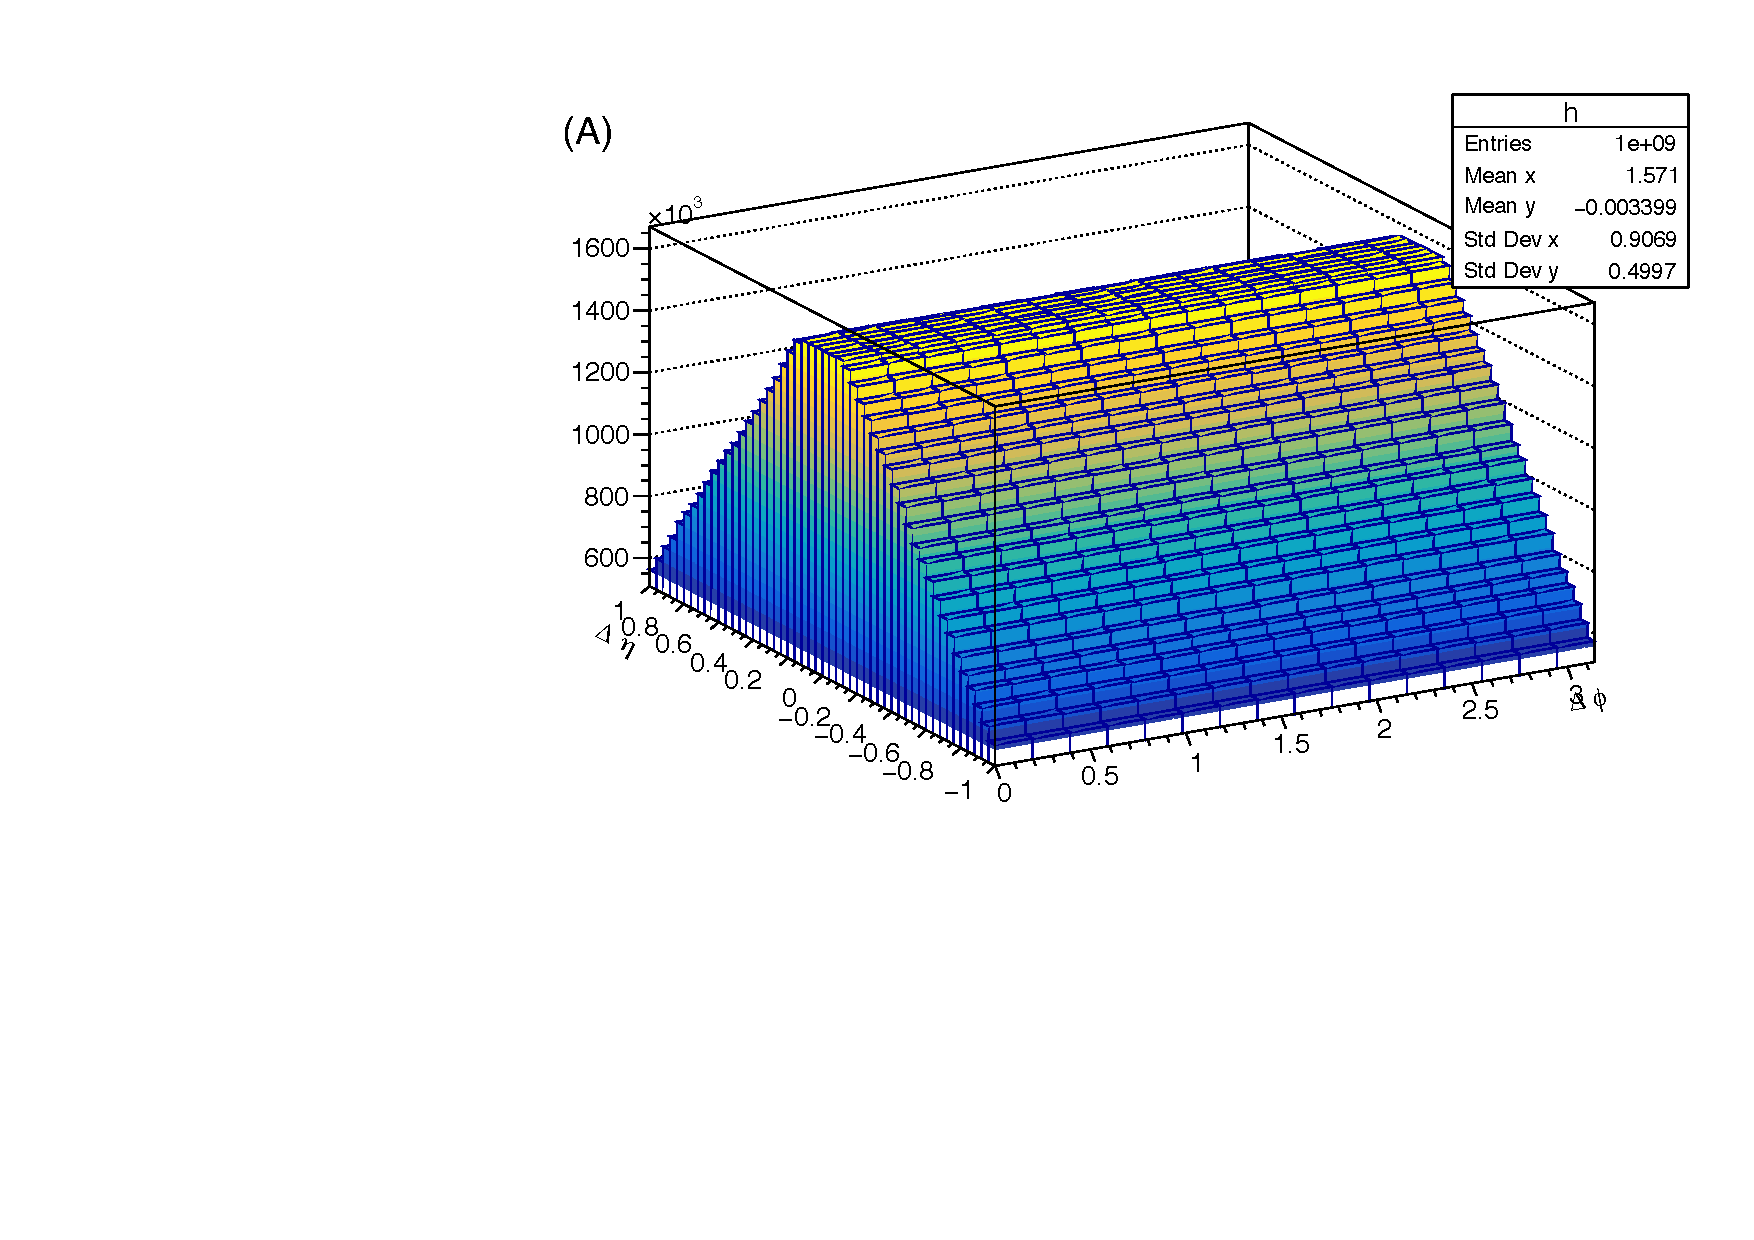
\includegraphics[width=0.49\textwidth]{Data_Analysis/EventMixing/toy_MC_no_holes.pdf}
	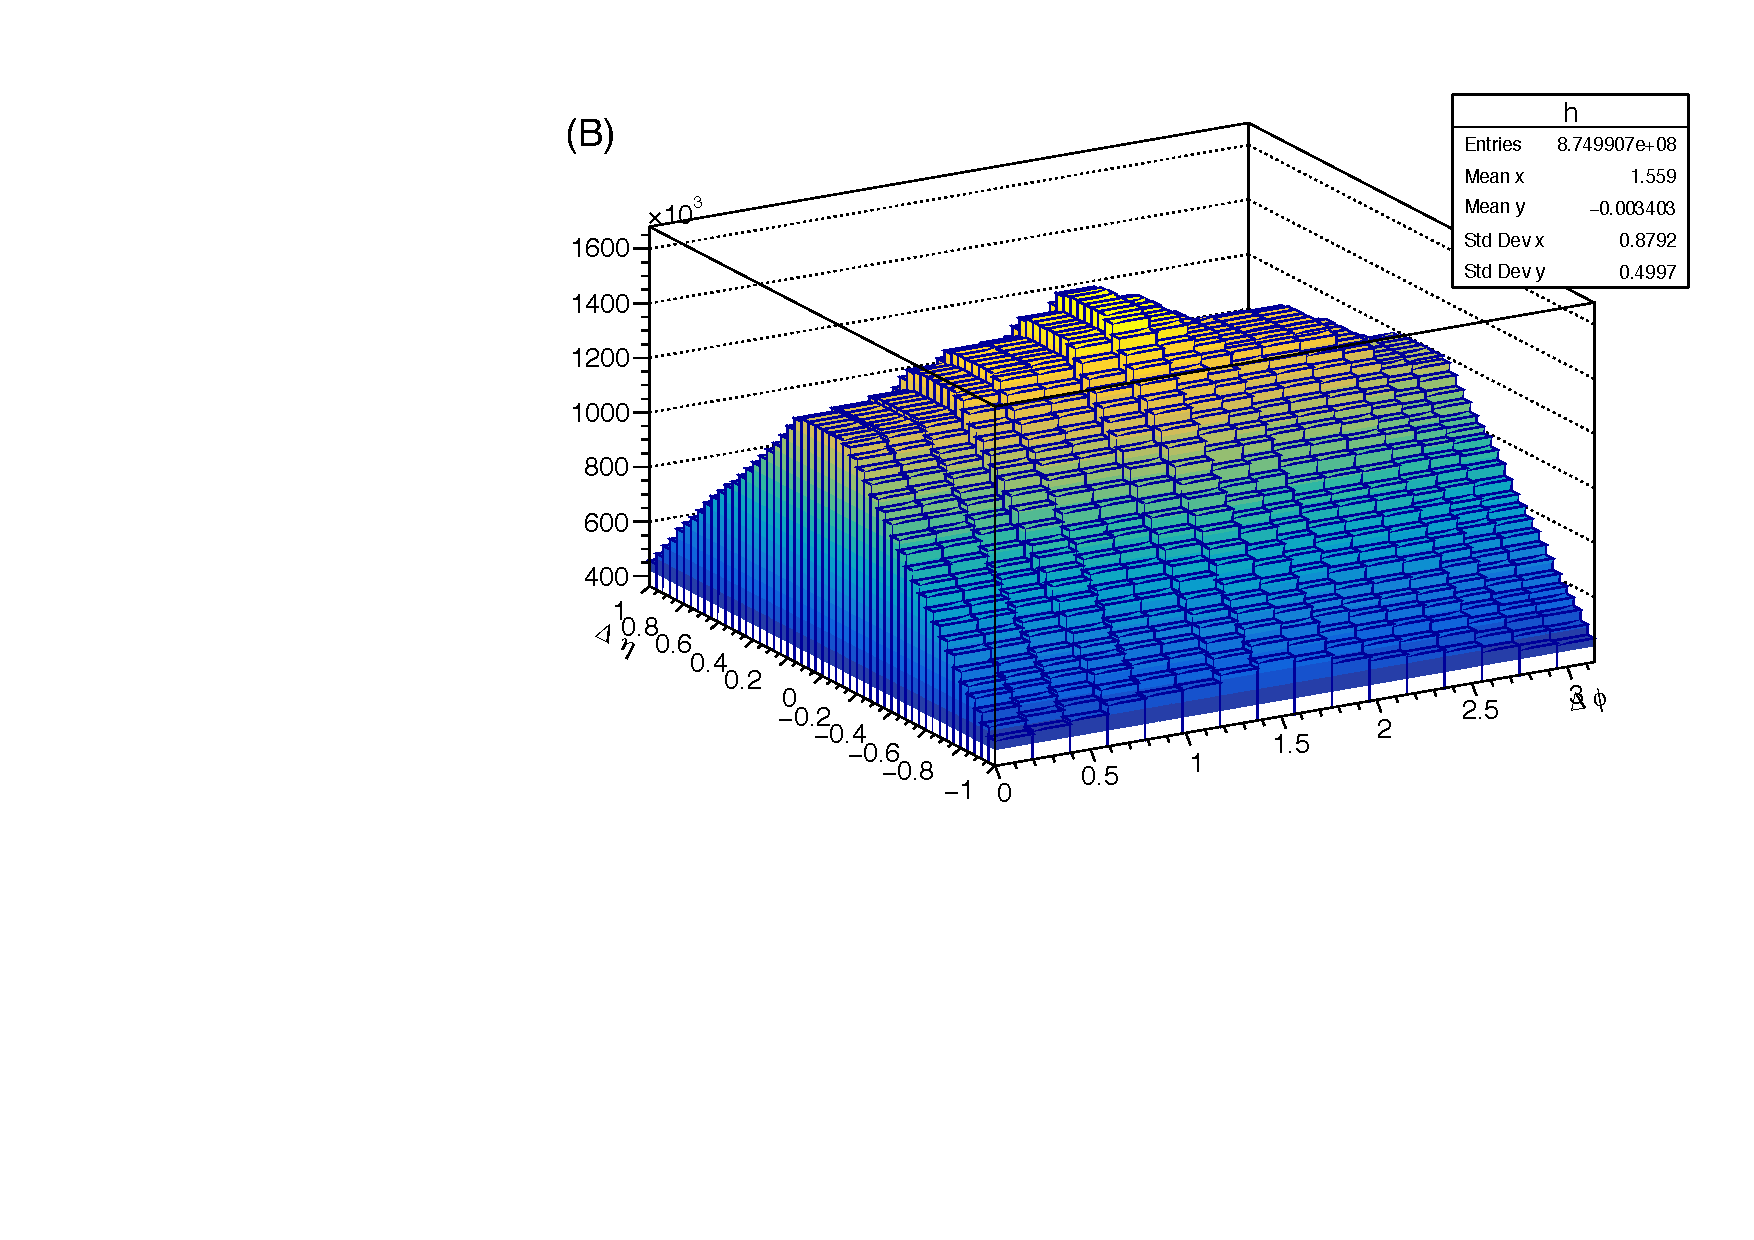
\includegraphics[width=0.49\textwidth]{Data_Analysis/EventMixing/toy_MC_holes.pdf}
  \caption{Toy Monte Carlo mixed-event correlation function. (Left) Photons are produced randomly within $0\textdegree \leq \varphi 107\textdegree$ and $ -0.67 \leq \eta \leq 0.67$ to roughly match the ALICE EMCal acceptance. Tracks are produced randomly for all values of $\varphi$ (between 0 and 360$\textdegree$) and $-0.8 < eta < 0.8$ to match the acceptance of an ideal ITS. (Right) Photons are generated in the same range as the left panel, however tracks have the additional constraint of excluding the range $ 25\textdegree< \varphi < 45\textdegree$ and $ 245\textdegree < \varphi < 270\textdegree$ in order to roughly approximate holes in the charged particle tracking efficiency, relative to the EMCal acceptance.} 
	\label{fig:toy}
\end{figure}

However, this flat distribution cannot be assumed, as previously seen in Figure \ref{fig:SR_2D} and now in Figure \ref{fig:toy_MC} (right). Dead areas or spots with a lower overall tracking efficiency accumulate over years of use at the LHC, and if large enough they can effect the pair-efficiency and therefore the mixed event correlations. This is shown in Figure \ref{fig:toy_MC_holes}. Both track and trigger photon \deltaeta~and \deltaphi~are constrained according to their respective detector acceptances, however additional holes in the $\varphi$ distribution of tracks are placed according to 2D tracking efficiency plot, Fig.~\ref{fig:phiEff}, Sec.~\ref{sec:tracking}.

\subsection{Binned Event Mixing}

Typically, events are binned according the their event information, centrality, z-vertex, flow (in PbPb), and then added to larger pools of events according to these bins. While it depends on the analysis, very common bin sizes are 5\%, 2cm for centrality and z-vertex. The gale-shapley pairing algorithm is novel for this use case, and thus a check was carried out in which the mixed event  correlation function was calculated using the standard binning method for event mixing.
\begin{figure}[htpb]
\center
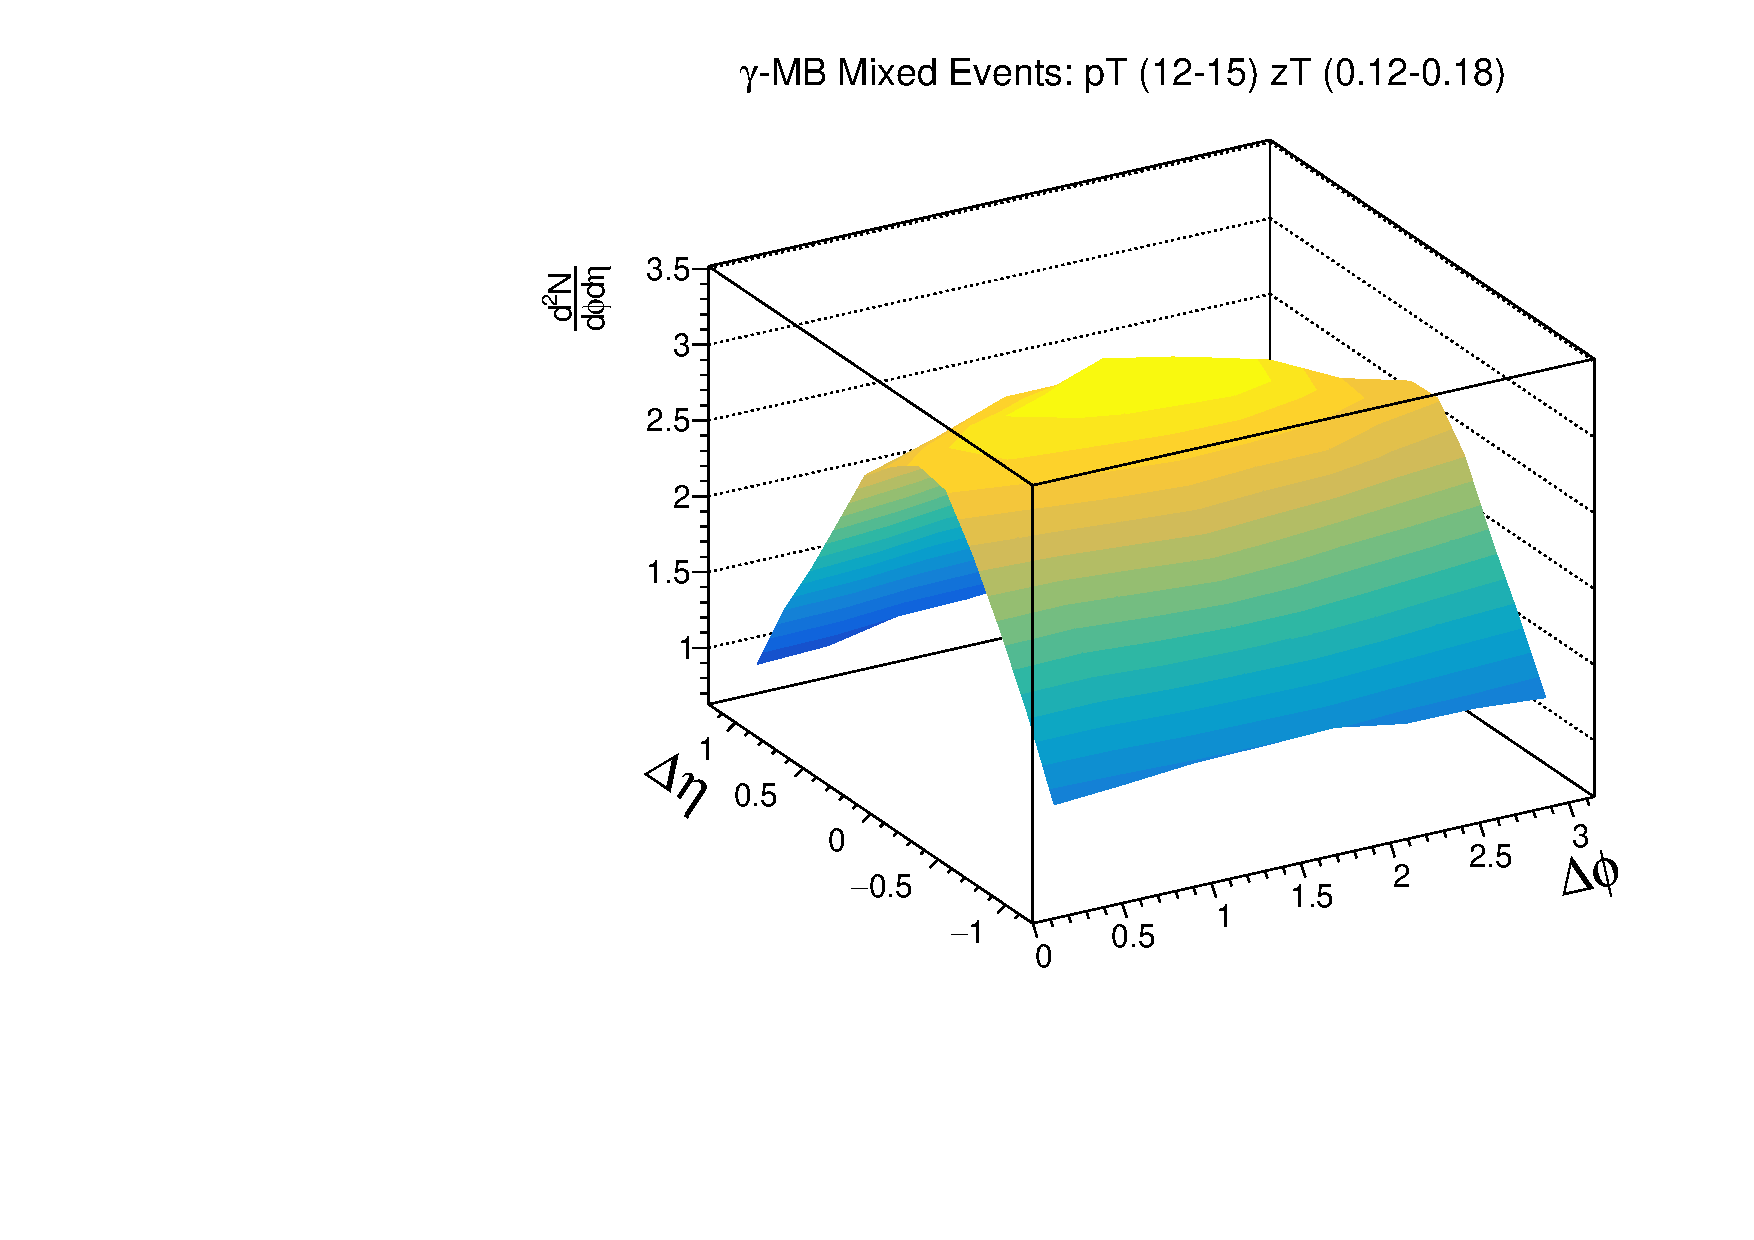
\includegraphics[width=0.7\textwidth]{Data_Analysis/EventMixing/2D_Bin_Corr.pdf}%
\caption{10 Mixed-Event correlation using the traditional binning method. The major features presented in the Gale-Shapley-Paired Mixed event correlation are reproduced in this low-statistics binned mixing check; The trapezoidal shape in $\Delta\eta$ and the non-uniformity in $\Delta\phi$ from holes in the ITS are reproduced.}
\label{BIN_Mixed_2D}
\end{figure}
\FloatBarrier

\section{Underlying Event Estimation}
The underlying event must be corrected for in two separate steps in this analysis. One is the pedestal in the correlation functions, attributed to correlating soft particles in the underlying event with the trigger isolated photon. The second is in the estimation of the underlying event density used in the isolation criteria. This section discusses checks on both corrections.

\subsection{Large \deltaeta~Check}

The ZYAM assumption is incredibly useful, as it indicates the overall magnitude of the background arising from the underlying event. It is, however, an assumption that must be checked. To check that the pedestal estimate using the ZYAM assumption truly corresponds to the amount of uncorrelated background, it is cross checked with another reasonable background estimation method.


As a check on the ZYAM procedure, one can take advantage of the fact that the UE-estimation is independent of $\Delta\eta$ and that that genuine correlations due to hard-scatterings decrease as $\Delta\eta$ increases. To this end, a region that is dominated by UE is selected, and then extrapolate back to the region that would normally contains both UE and hard-scattering contribution. The UE is estimated by projecting the large $\Delta\eta$ region defined as $0.8 < |\Delta\eta| < 1.4$ onto the $\Delta\varphi$ axis. To minimize bias from the isolation cut as well as the away side jet peak, the uncorrelated background is estimated from the projection in the region $0.4 < \Delta\varphi < 1.4$. This $\Delta\varphi\Delta\eta$ region is illustrated in Figure~\ref{fig:LE_Map}. 

This region is chosen because particles from the same hard scattering are very unlikely to have a small \deltaphi and large \deltaeta in the absence of flow effects. This is because the nearside jet peak arises from the autocorrelation of the particles within a jet, i.e. it is sensitive only to the individual characteristics of a single parent parton and it's fragmentation process. Therefore, the near side jet peak is observed as a sharp peak at small \deltaphi and \deltaeta. The away side jet ridge however, is the result of correlating particles between jets, and is therefore sensitive to the \kt asymmetry of the two colliding partons: The partons in the initial system  do not \textit{necessarily} have 0 \pt. Both partons can have an initial transverse momentum, \kt, that makes up a component of their overall momentum fraction of the nucleon, bjorken-x, and the resulting scattering becomes more spread out in \deltaeta. For this reason, a region in small \deltaphi and large \deltaeta will be dominated by the underlying event, as it avoids the away-side ridge, and the sharp near side jet peak.
%In heavy ion collisions, particles with a large separation in $\eta$ are unlikely to originate from the same hard scattering.\subsection{Underlying Event Subtraction}. The small fraction of partons that suffer hard perturbative interactions directly result in the production of high \pt particles. While the charged particles from different jets for example will be separated in \deltaphi in the simplest back-to-back scattering picture, both jets will tend to be around mid-rapidity. Kinematically, particles with high \pt will tend to be located at mid-rapidity. This is because particles with high \pt will tend to have a larger component their overall momentum will be transverse to the beam direction. Particles that are completley transverse to the beam direction will be at $\eta=0$. Therefore, particles with high transverse momentum resulting from a hard scattering will tend to be at mid rapidity, and have 

\begin{figure}[htpb]
\center
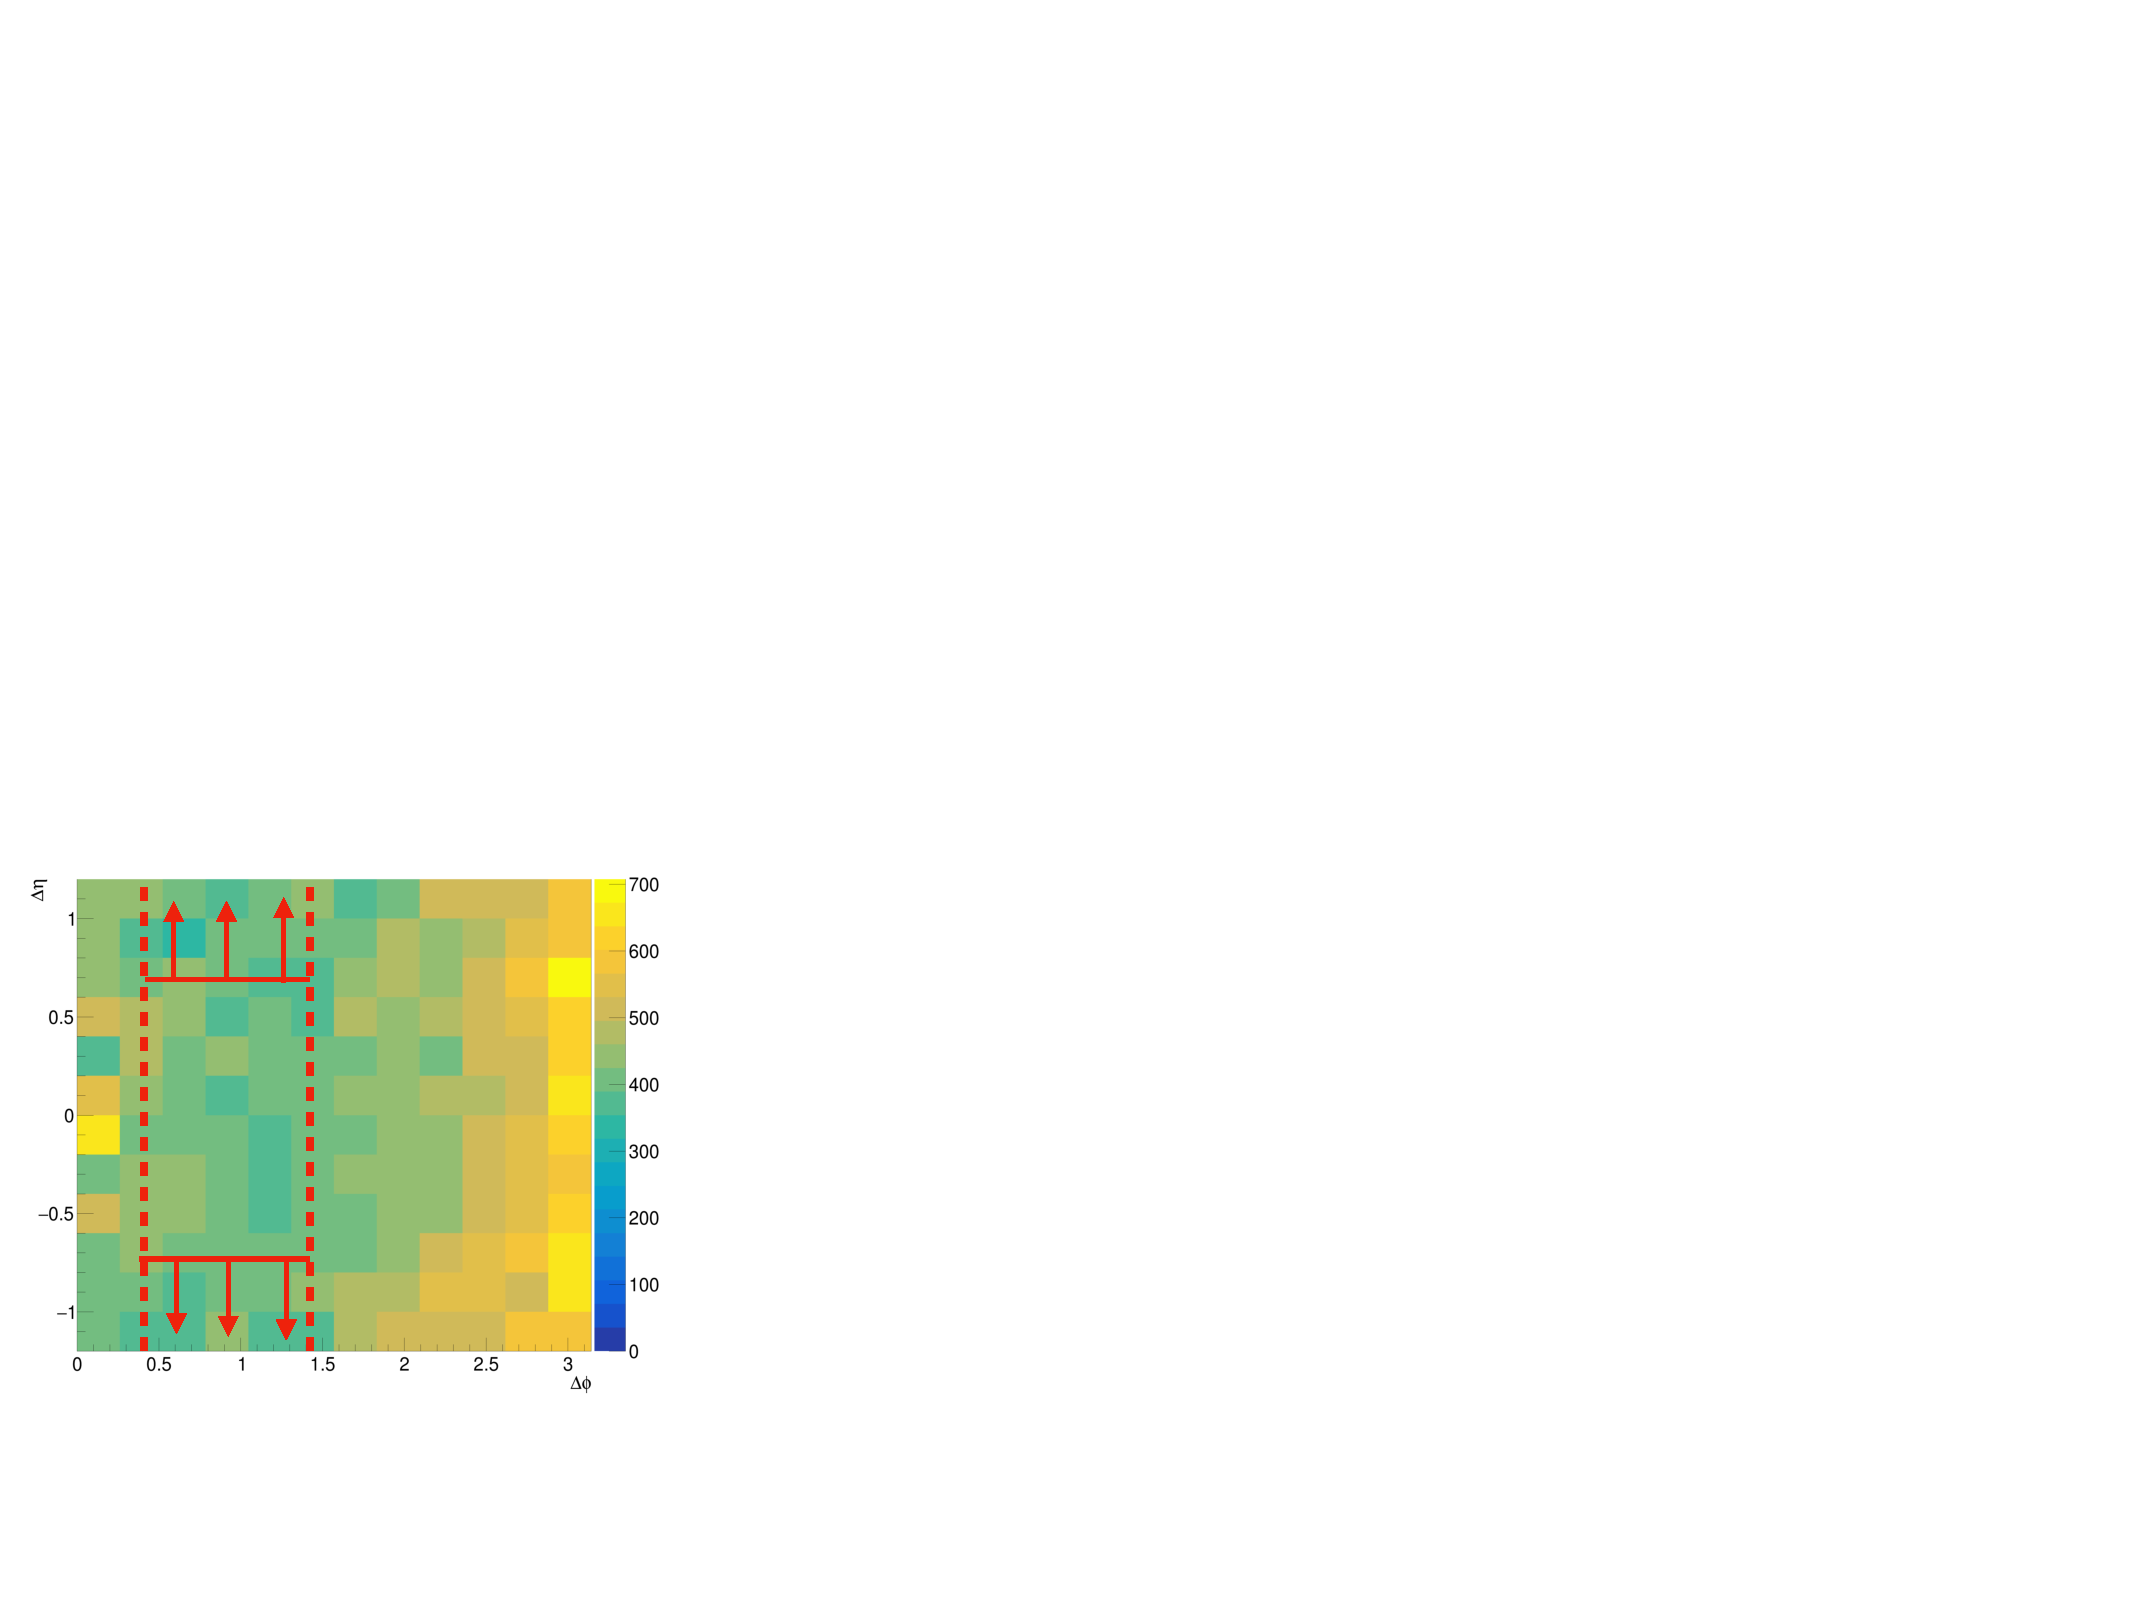
\includegraphics[width=0.5\textwidth]{Data_Analysis/EventMixing/LE_map.pdf}
\caption{The 2D region used to calculate the uncorrelated background. The $\Delta\varphi$ region is chosen to avoid the away side jet peak, as well as the isolation region of R$=$0.4. The $\Delta\eta$ region is chosen assuming that genuine correlations from hard-scatterings decrease as $\Delta\eta$ increases. The large $\Delta\eta$ is projected onto the $\Delta\varphi$ axis, and then averaged within region of 0.4 $<\Delta\varphi<$ 1.4. ZYAM is estimated in the region $ 0.4 < \Delta\varphi < 1.4$, but for the full $\Delta\eta$ range ($-1.2 < \Delta\eta < 1.2$).}
\label{fig:LE_Map}
\end{figure}

The statistical uncertainty in the UE estimate method is taken as a systematic uncertainty for $\Delta\varphi$ correlations as it is completely correlated bin-to-bin in $\Delta\varphi$.
Figure~\ref{small_uncorr} shows the two UE estimates compared with the isolated photon-hadron $\Delta\varphi$ 
%bvj projections 
correlations for only 2 \zt~bins in order to show detail. The full detail of the two UE estimates is shown in Tables~\ref{tab:UE_Average} for pp and \pPb~data. The two estimates are consistent within uncertainties for almost all \zt~bins in both pp and \pPb~data. For the only case where a significant disagreement is observed, which is for the lowest \zt~bin in \pPb~data, the difference is summed in quadrature as an additional systematic uncertainty. 

\begin{figure}[htpb]
	\center
	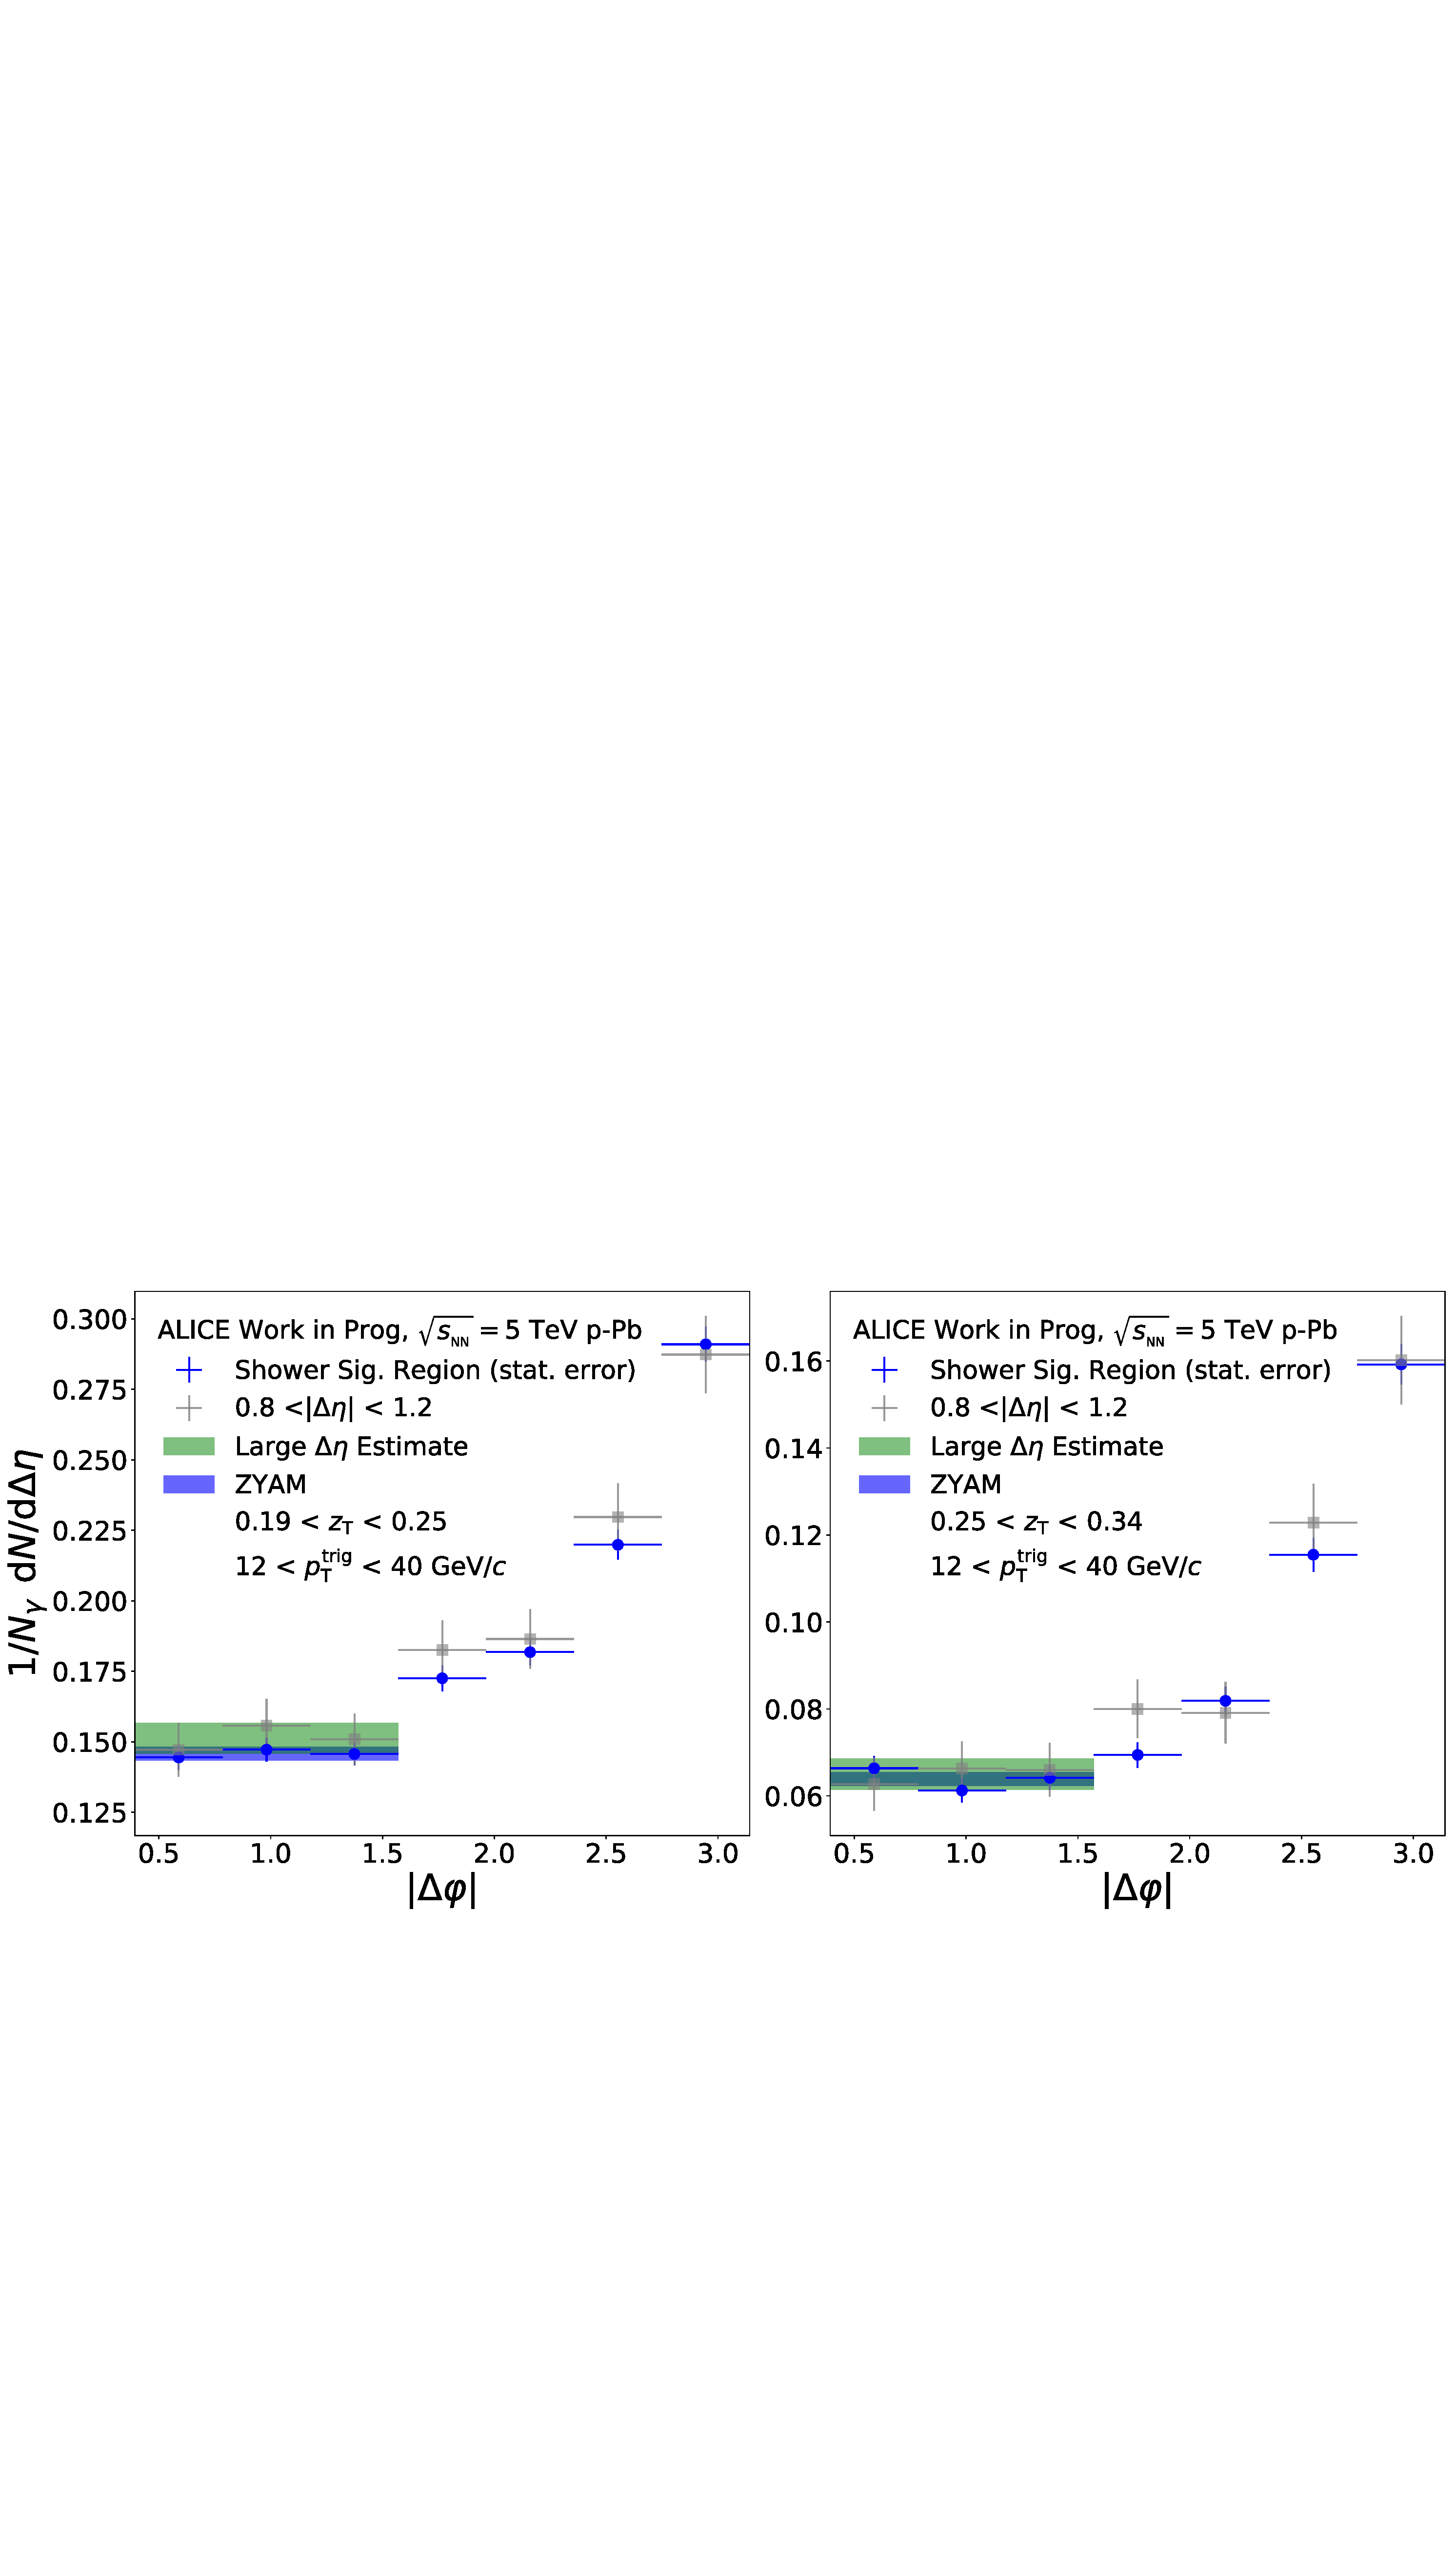
\includegraphics[width=.99\textwidth]{Data_Analysis/G-H_New/UE_Plot_p-Pb_Single.pdf}
\caption{Projections of the $\gammaiso$--hadron correlations in \pPb~collisions in 2 $\zt$~bins after correlated subtraction with UE estimates plotted. The grey points represent the large $\Delta\eta$ region ( $ 0.8 < |\Delta\eta| < 1.2$) projected onto the $\Delta\varphi$ axis. The blue band represents the region used to calculate ZYAM and the green band represents the region of large $\Delta\eta$ points used to calculate the Large $\Delta\eta$ estimate.}
\label{small_uncorr}
\end{figure}


\begin{table}
   \centering
      \caption{Summary of UE-pedestal estimates with ZYAM and the $\Delta\eta$ method for various $\zt$ bins, as well as the difference between LE and ZYAM estimates. The background estimate is shown in units of pairs per trigger. The uncertainty quoted is statistical only.}
   \begin{tabular*}{1.0\columnwidth}{@{\extracolsep{\fill}}lccc@{}}
    \hline
		$z_\mathrm{T}$ interval & ZYAM  & Large $\Delta\eta$ & Difference\\
		\hline
		pp & & \\
		\hline
0.06 - 0.08 & 0.480 $\pm$ 0.007 & 0.472 $\pm$ 0.015 & 0.008 $\pm$ 0.016\\
0.08 - 0.11 & 0.347 $\pm$ 0.006 & 0.346 $\pm$ 0.012 & 0.000 $\pm$ 0.014\\
0.11 - 0.14 & 0.219 $\pm$ 0.005 & 0.209 $\pm$ 0.010 & 0.009 $\pm$ 0.011\\
0.14 - 0.19 & 0.131 $\pm$ 0.004 & 0.129 $\pm$ 0.008 & 0.002 $\pm$ 0.008\\
0.19 - 0.25 & 0.063 $\pm$ 0.002 & 0.058 $\pm$ 0.005 & 0.005 $\pm$ 0.006\\
0.25 - 0.34 & 0.030 $\pm$ 0.002 & 0.025 $\pm$ 0.003 & 0.005 $\pm$ 0.004\\
0.34 - 0.45 & 0.013 $\pm$ 0.001 & 0.015 $\pm$ 0.003 & 0.002 $\pm$ 0.003\\
0.45 - 0.60 & 0.006 $\pm$ 0.001 & 0.005 $\pm$ 0.002 & 0.001 $\pm$ 0.002\\
	\hline 
	\pPb & & \\
	\hline
0.06 - 0.08 & 1.142 $\pm$ 0.006 & 1.190 $\pm$ 0.013 & 0.047 $\pm$ 0.014\\
0.08 - 0.11 & 0.855 $\pm$ 0.005 & 0.864 $\pm$ 0.011 & 0.010 $\pm$ 0.012\\
0.11 - 0.14 & 0.557 $\pm$ 0.004 & 0.566 $\pm$ 0.009 & 0.009 $\pm$ 0.010\\
0.14 - 0.19 & 0.318 $\pm$ 0.003 & 0.317 $\pm$ 0.007 & 0.001 $\pm$ 0.007\\
0.19 - 0.25 & 0.151 $\pm$ 0.002 & 0.159 $\pm$ 0.005 & 0.009 $\pm$ 0.005\\
0.25 - 0.34 & 0.062 $\pm$ 0.001 & 0.062 $\pm$ 0.003 & 0.000 $\pm$ 0.003\\
0.34 - 0.45 & 0.022 $\pm$ 0.001 & 0.021 $\pm$ 0.002 & 0.001 $\pm$ 0.002\\
0.45 - 0.60 & 0.007 $\pm$ 0.000 & 0.006 $\pm$ 0.001 & 0.001 $\pm$ 0.001\\

   \end{tabular*}
   \label{tab:UE_Average}
\end{table}


\subsection{Checks on UE Estimate with Standard ALICE Tracking}
As discussed in Section~\ref{sec:tracking}, the TPC had space-charge distortions during the 2013 \pPb~run that resulted in a drop in efficiency for tracking beyond 4 GeV, which limits the ability to use it for the correlation measurements. However, the TPC tracks can still be used for low $\pt$ tracking, which is the relevant region for underlying-event and isolation measurements. 

Figure~\ref{fig:pPb_its_tpc_rho} shows the $\rho$  and isolation distributions measured with ITS-only and TPC+ITS tracks in \pPb~data. The $\rho$ distributions are very similar; the means of $\rho$ to be 3.129 GeV and 3.202 GeV for ITS and TPC+ITS $\rho$ values respectively. This is expected because the UE-estimation is dominated by tracks with low momentum, and while the ITS tracking resolution is poorer, the smearing effects are relative small at low momentum. There are some differences in the isolation distribution, however, that can be attributed to the worse momentum resolution for the ITS-only tracks as the isolation is sensitive to higher $\pt$~tracks where the momentum resolution worsening is more significant. 

\begin{figure}[hbtp]
	\center
	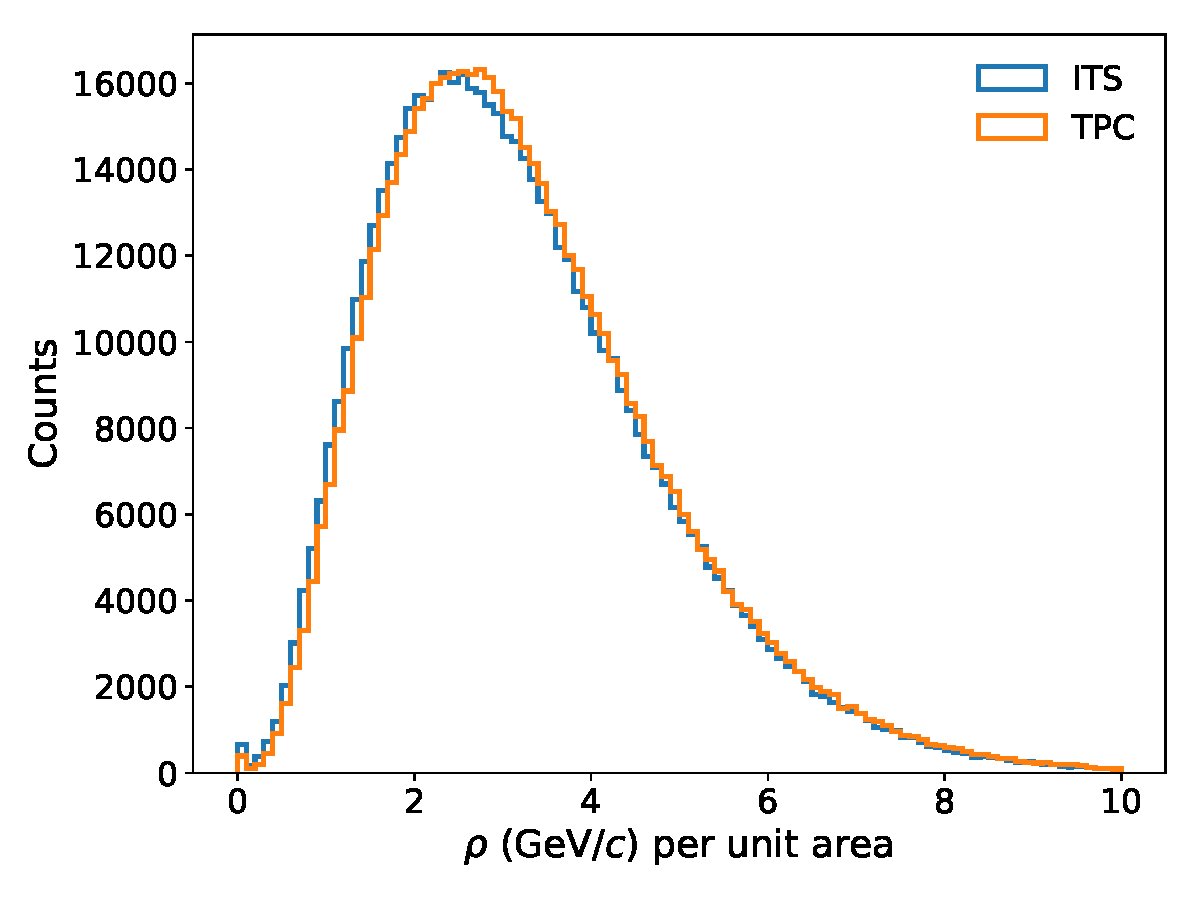
\includegraphics[width=0.49\textwidth]{Checks_Systematics/UEestimate_Skimmed_13def.pdf}
		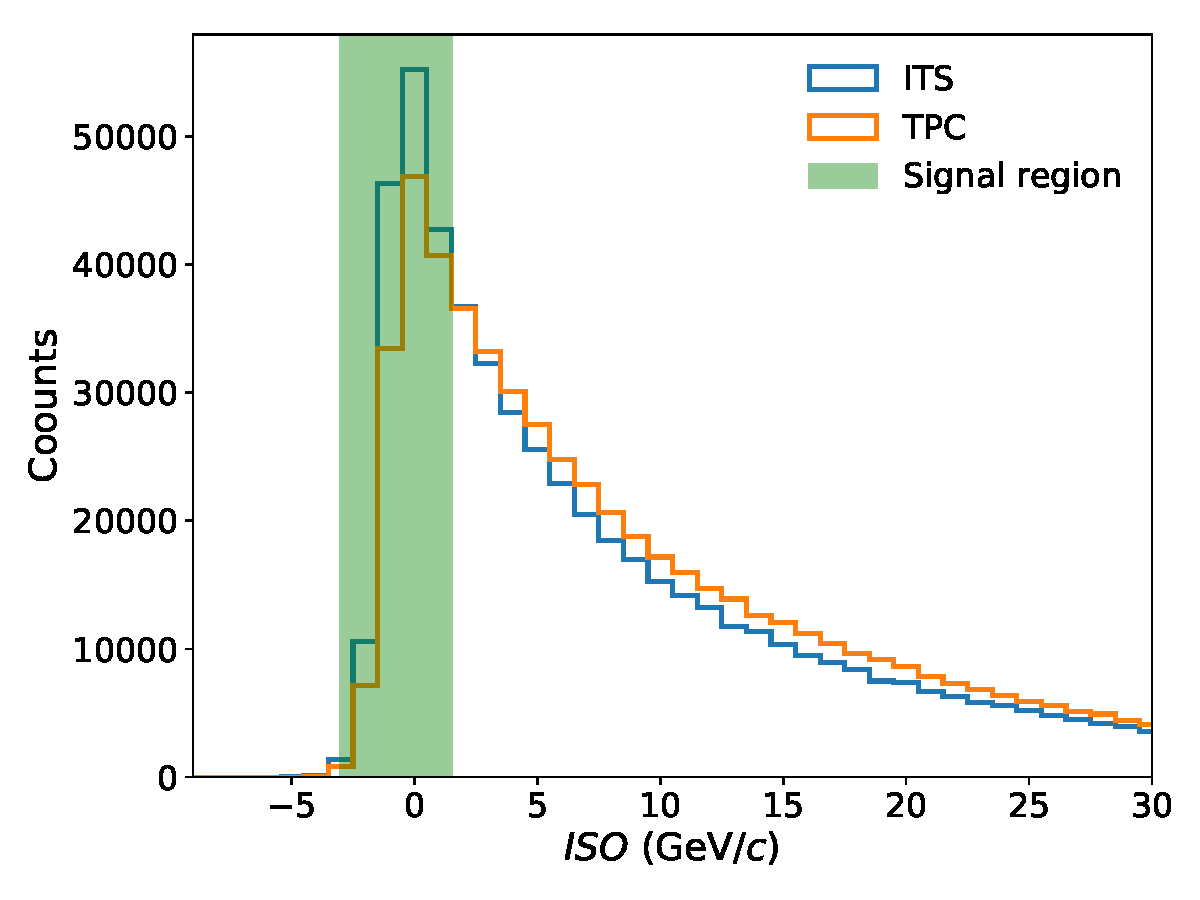
\includegraphics[width=0.49\textwidth]{Checks_Systematics/IsolationTPC_Skimmed_13def.pdf}
	\caption{Transverse momentum density (left panel) and isolation distributions (right panel) determined with ITS tracks (in blue) and TPC+ITS tracks (in orange) in \pPb~data.}
	\label{fig:pPb_its_tpc_rho}
\end{figure}

For simplicity the same threshold of 1.5 \GeVc~is used for the $\gammaiso$~candidates for both the ITS-only and ITS+TPC tracks. The ITS+TPC tracks leads to a better rejection of the background, which leads to an increased photon purity. This is shown in Figure~\ref{fig:ComparisonTPCITSiso_purity}. 

\begin{figure}[hbt]
	\center
	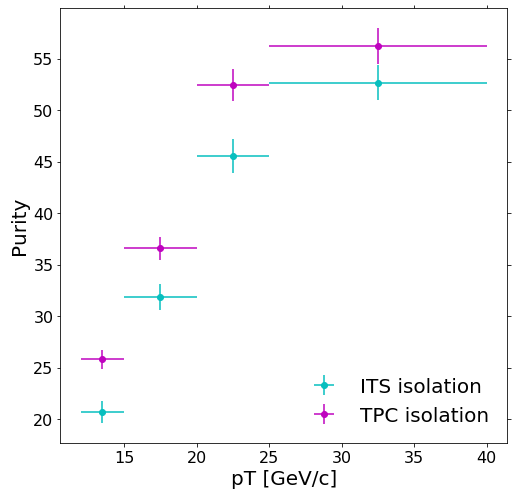
\includegraphics[width=0.49\textwidth]{Checks_Systematics/PurityITSTPC.png}
	\caption{Comparison of purity obtained in \pPb~collisions with isolation variable obtained with ITS-only tracks (purple) and with ITS+TPC tracks (cyan). The error bars represent statistical uncertainty only. }
	\label{fig:ComparisonTPCITSiso_purity}
\end{figure}

The main results (correlation function) were checked in \pPb~data by performing the analysis with isolation variable, UE estimate, and corresponding purity values calculated separately for ITS-only tracks and for ITS+TPC tracks. As shown in Figure~\ref{fig:ComparisonTPCITSiso_frag}, the results are consistent. A slightly better statistical uncertainty is obtained when including TPC (a relative uncertainty of 22$\%$ to 41$\%$ depending on \zt~vs 24$\%$ to $51\%$ for the ITS case), which an be attributed to the corresponding higher purity. However, these slightly better statistical uncertainties do not change the main result of this study. For consistency with pp results (where one cannot use ITS+TPC tracks because the TPC was not read out), results for ITS-only tracks was chosen for the final analysis. 

\begin{figure}
	\center
	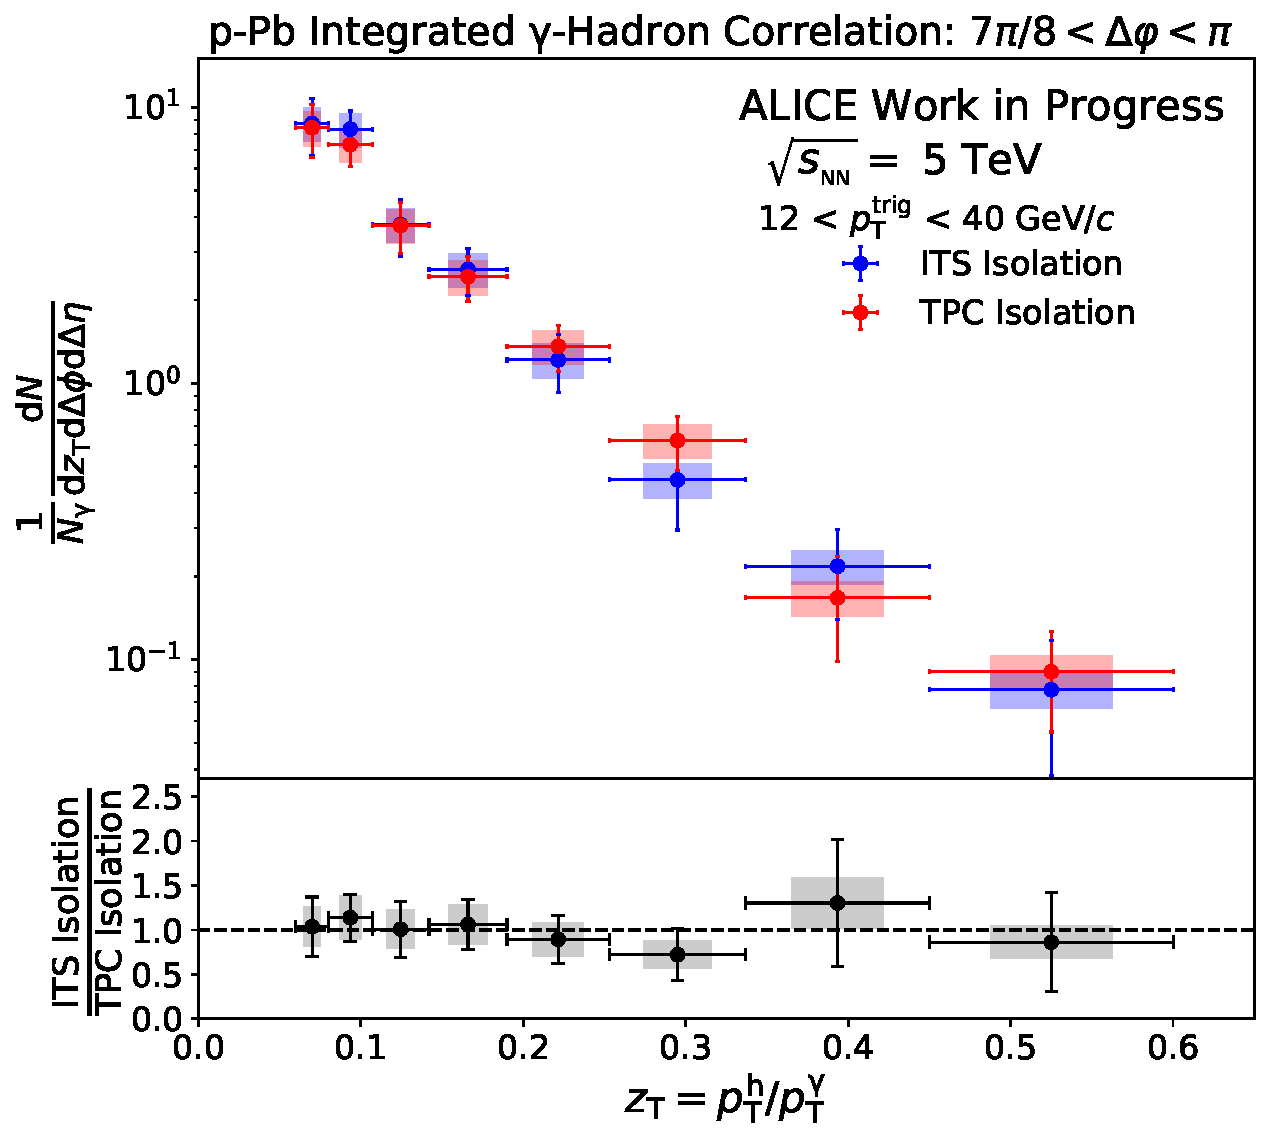
\includegraphics[width=0.49\textwidth]{Checks_Systematics/ISO_Compare_Final_FFunction_and_Ratio}
	\caption{Comparison of fragmentation function measurement in \pPb~collisions with isolation variable obtained with ITS-only tracks (blue) and with ITS+TPC tracks (red).}
	\label{fig:ComparisonTPCITSiso_frag}
\end{figure}

This study comparing ITS-only tracking and ITS+TPC tracks serves as a check against possible biases due to worse momentum resolution or fake rate of the ITS-only tracking. Because consistent results are obtained with the standard ITS+TPC tracking, an additional systematic uncertainty is not assigned for the tracking performance on UE-estimate and isolation variables. 

% This asymmetry in the kT of the incoming partons results in a broader gausian in \deltaphi~than the nears side peak. 

% The difference in overall momentum fraction in the two partons is responsible for the away-side ridge spanning a very large region in \deltaeta.

\section{Purity}
\subsection{Systematic Uncertainties of the Purity Measurement}
\label{sec:puritysystematics}
There are two assumptions underlying the template fit procedure. The first is that the signal template from simulations is correct. The second is that the shape of the background estimated from the anti-isolated sideband, with the correction estimated from simulations, reflects the shape of the background in the signal region. In other words, the assumption is that the correlation between the shower shape and isolation variables can be corrected for via an appropriate simulation. The dominant sources of systematic uncertainty on the purity calculation are described in this section and can be summarized as follows: the signal template, the sideband region selection, and the background template correction. The effect of varying the cluster selection requirements were investigated, but it was found that the variations on the purity measurements are much smaller than the other sources of systematic uncertainties investigated here. Therefore, they are neglected. This is shown in Sec.~\ref{sec:clustercutselectionvariation}. 

\subsection{Signal Template}
The systematic uncertainty on the purity calculation arising from imperfections in the signal template is estimated by using a data-driven template fit. To this end, the range of the $\chi^{2}$ fit to the background-dominated region of the shower-shape distribution is restricted (0.4--1.5 for $\lambdasquare$) and the background template is used only to fit the isolated data with the normalization as the only free parameter. In order to factorize the effect of the MC-correction to the background template, that correction is not applied here for this study. Once the background normalization is fitted, the signal is considered to be the integral of the isolated data minus the integral of the background, both in the signal region of the shower-shape variable. 

Figure~\ref{BkgOnlyFit_pPb} shows the results obtained with this method in pp and \pPb~data. There appears to be some systematic pattern in the residuals, which can be attributed to the decision of not applying the MC-correction to the background template for this study. 

\begin{figure}[htpb]
\center
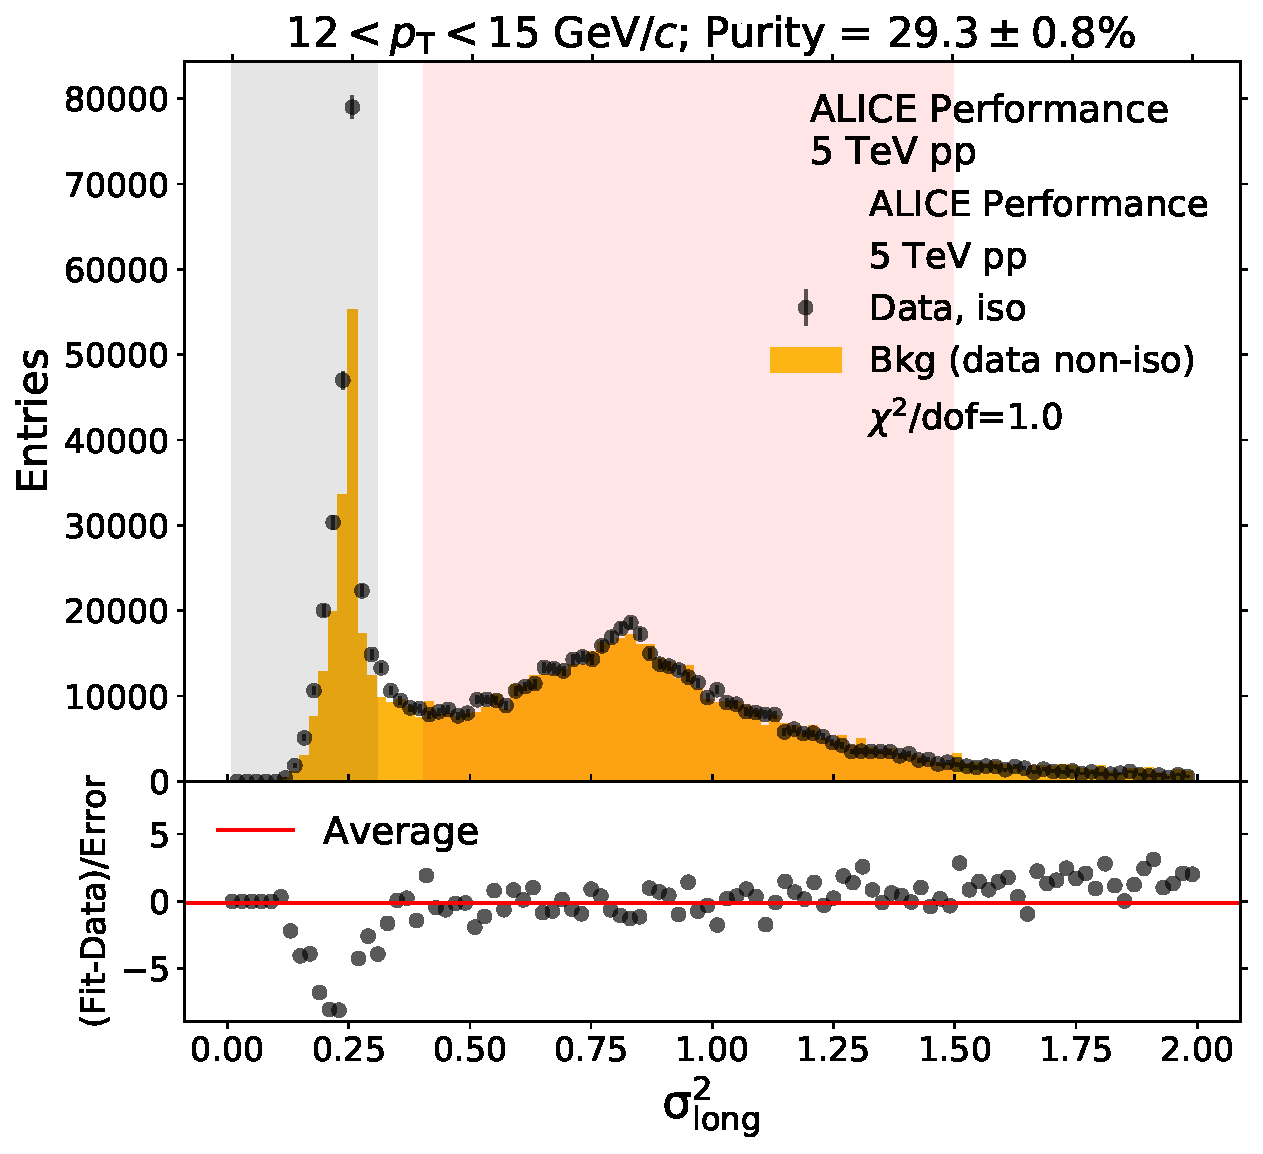
\includegraphics[width=0.38\textwidth]{Data_Analysis/Purity/bf-example-pp-cluster_Lambda-12-15.pdf}
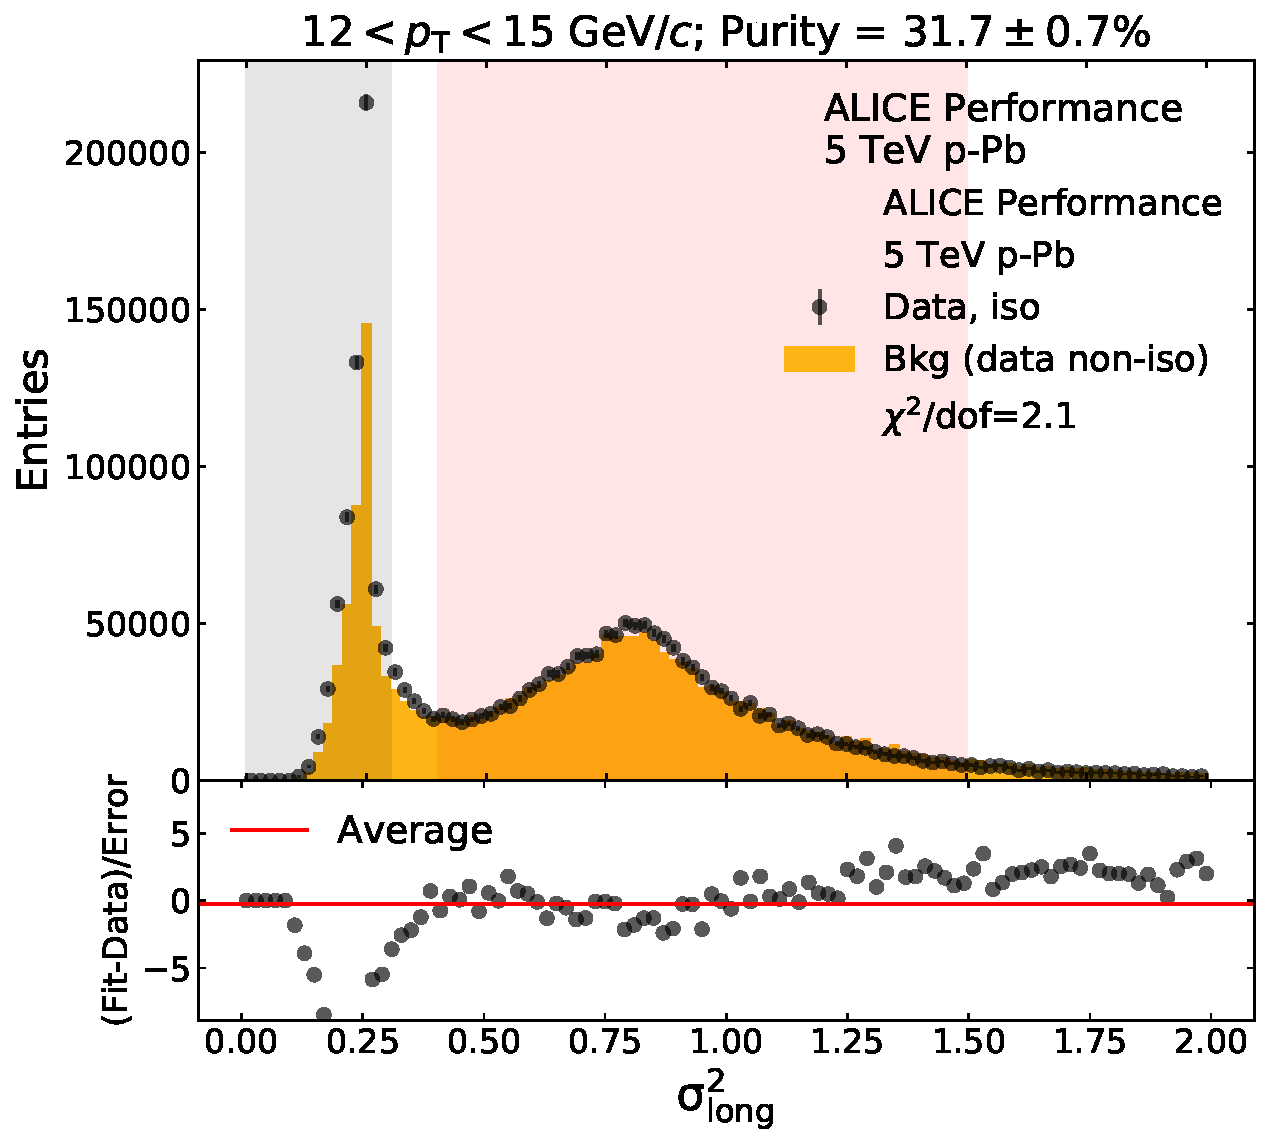
\includegraphics[width=0.38\textwidth]{Data_Analysis/Purity/bf-example-p-Pb-cluster_Lambda-12-15.pdf}
\\
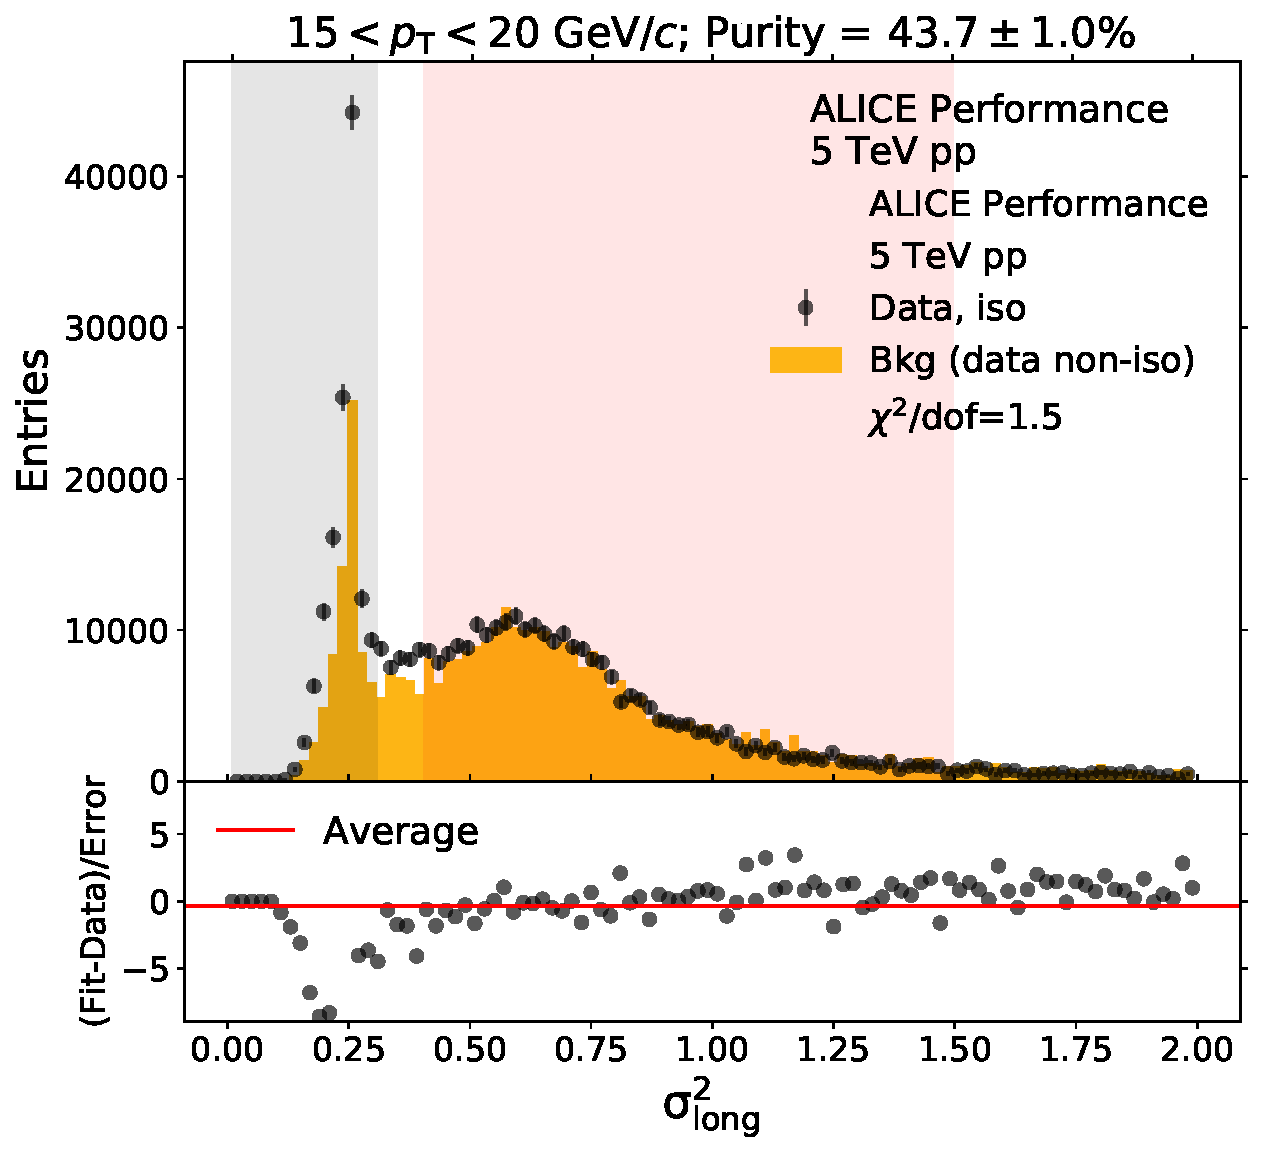
\includegraphics[width=0.38\textwidth]{Data_Analysis/Purity/bf-example-pp-cluster_Lambda-15-20.pdf}
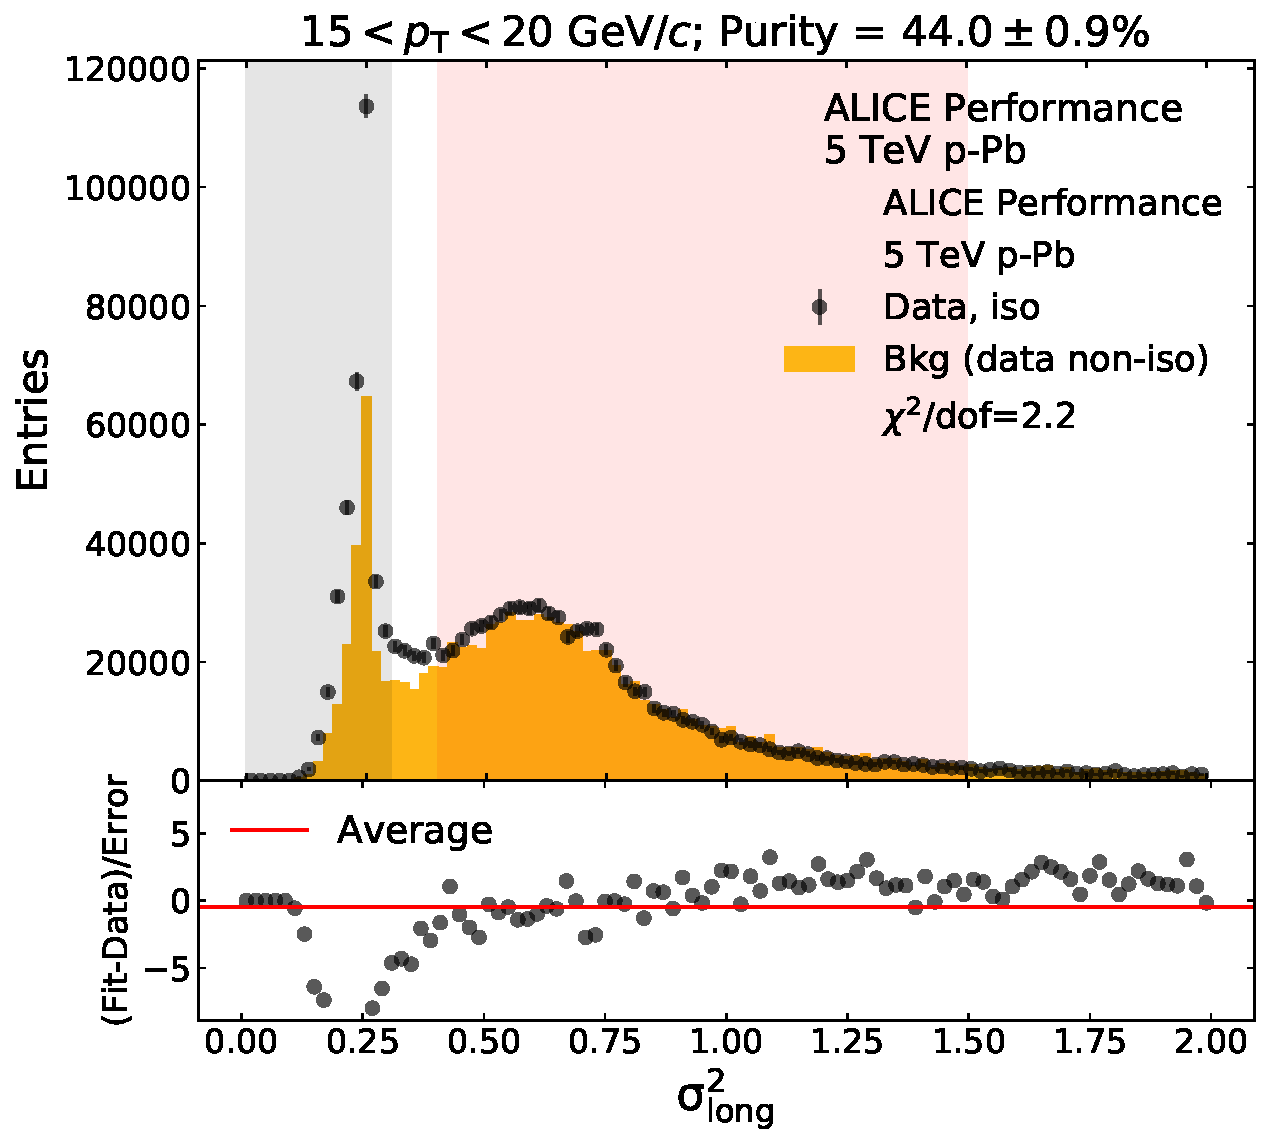
\includegraphics[width=0.38\textwidth]{Data_Analysis/Purity/bf-example-p-Pb-cluster_Lambda-15-20.pdf}
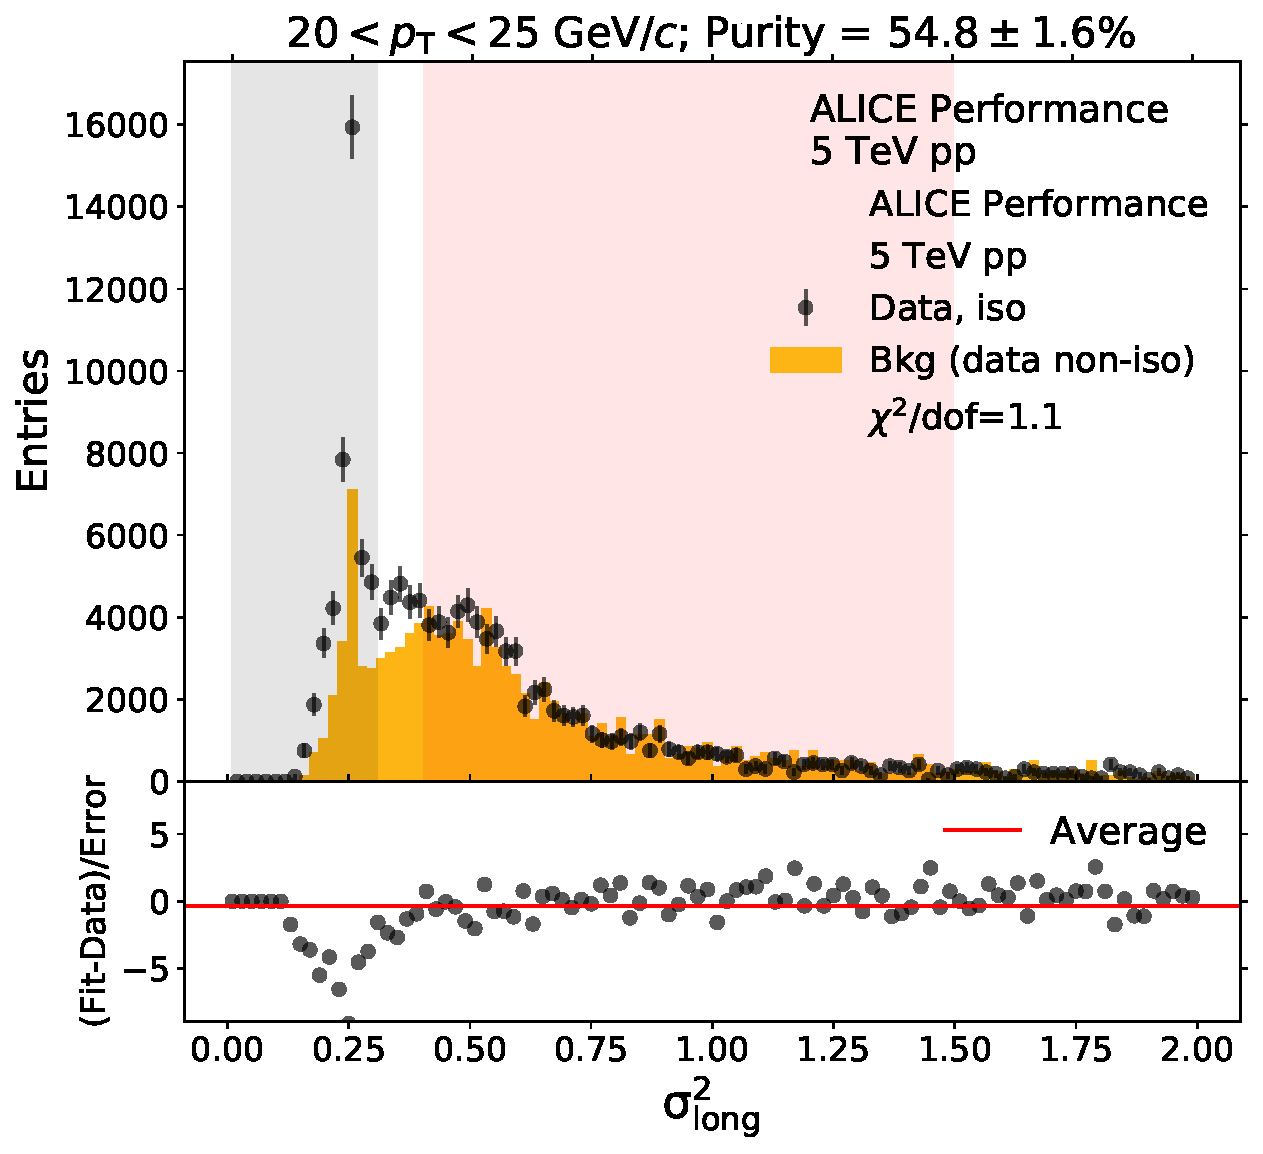
\includegraphics[width=0.38\textwidth]{Data_Analysis/Purity/bf-example-pp-cluster_Lambda-20-25.pdf}
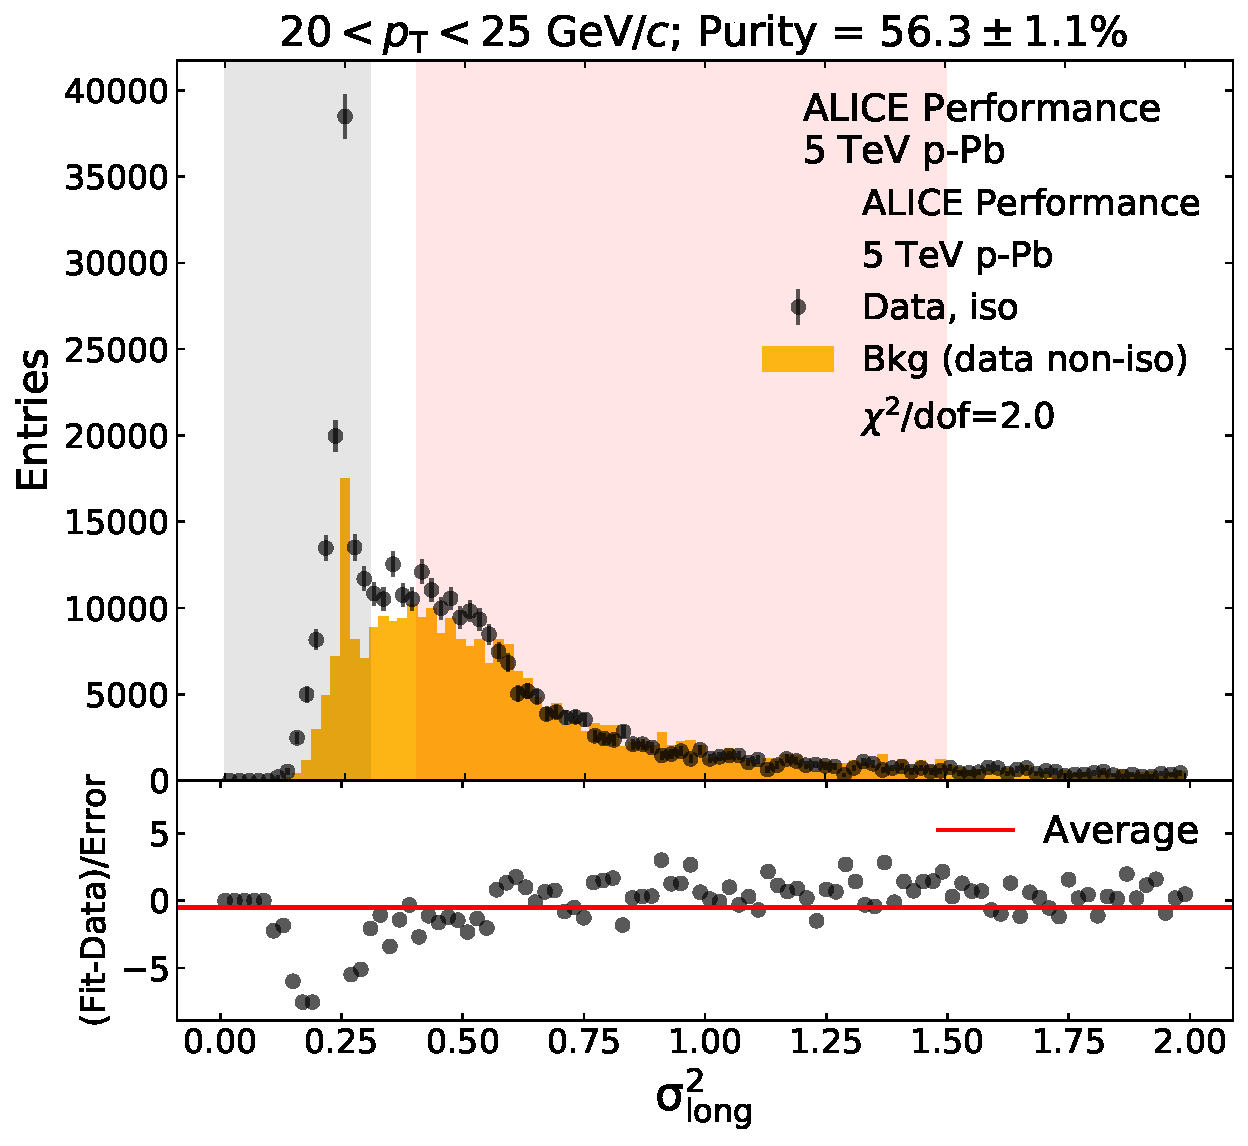
\includegraphics[width=0.38\textwidth]{Data_Analysis/Purity/bf-example-p-Pb-cluster_Lambda-20-25.pdf}
\\
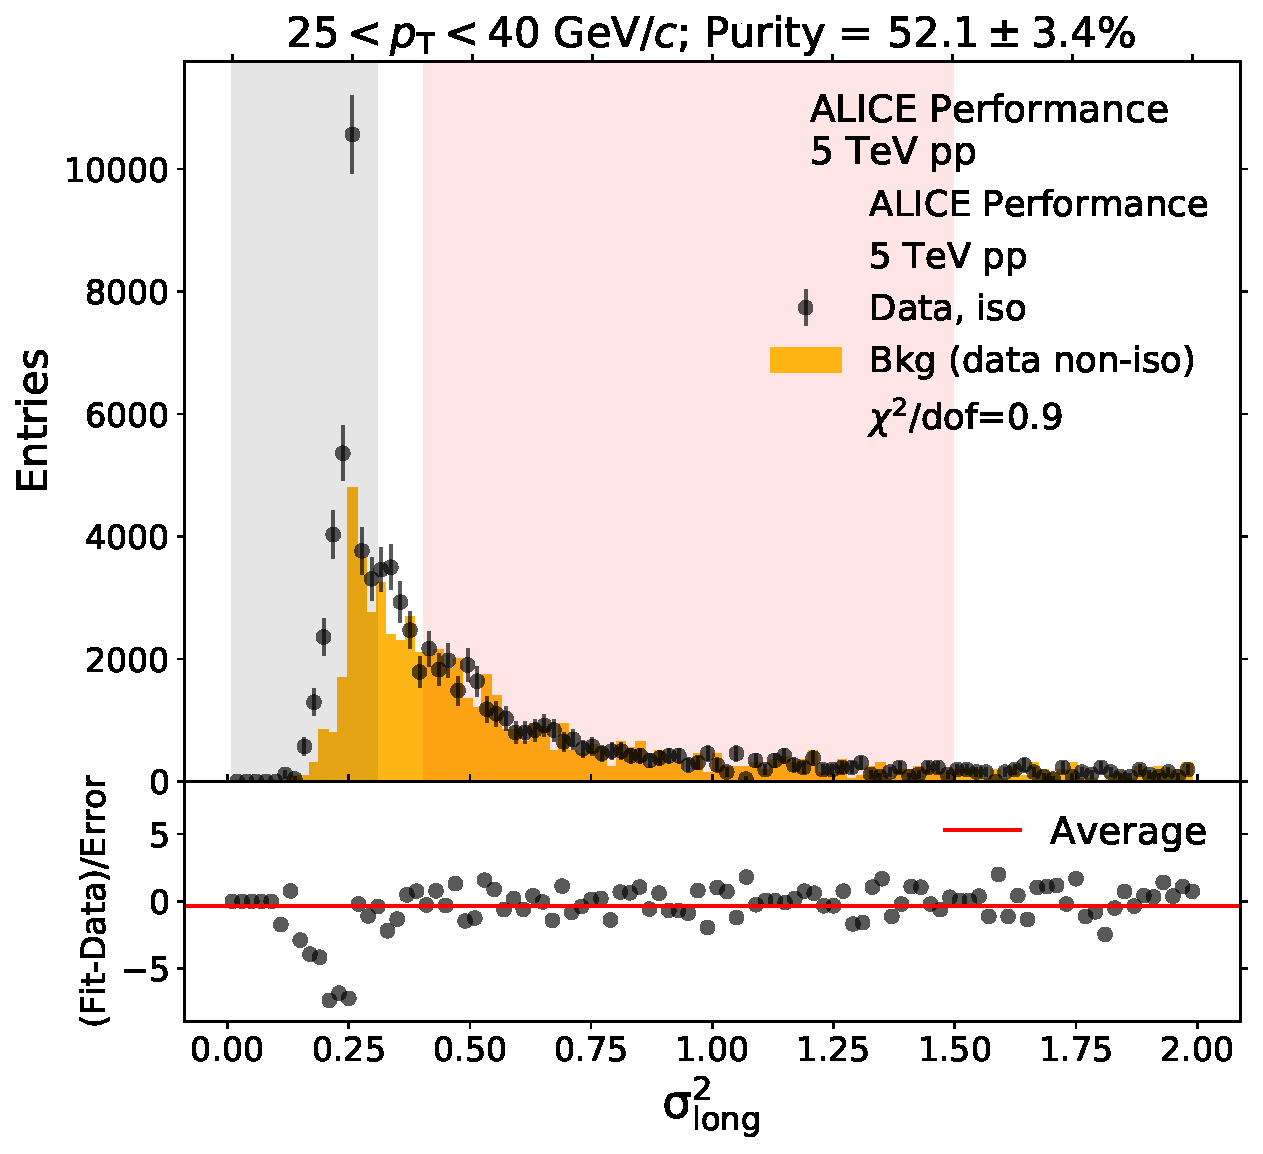
\includegraphics[width=0.38\textwidth]{Data_Analysis/Purity/bf-example-pp-cluster_Lambda-25-40.pdf}
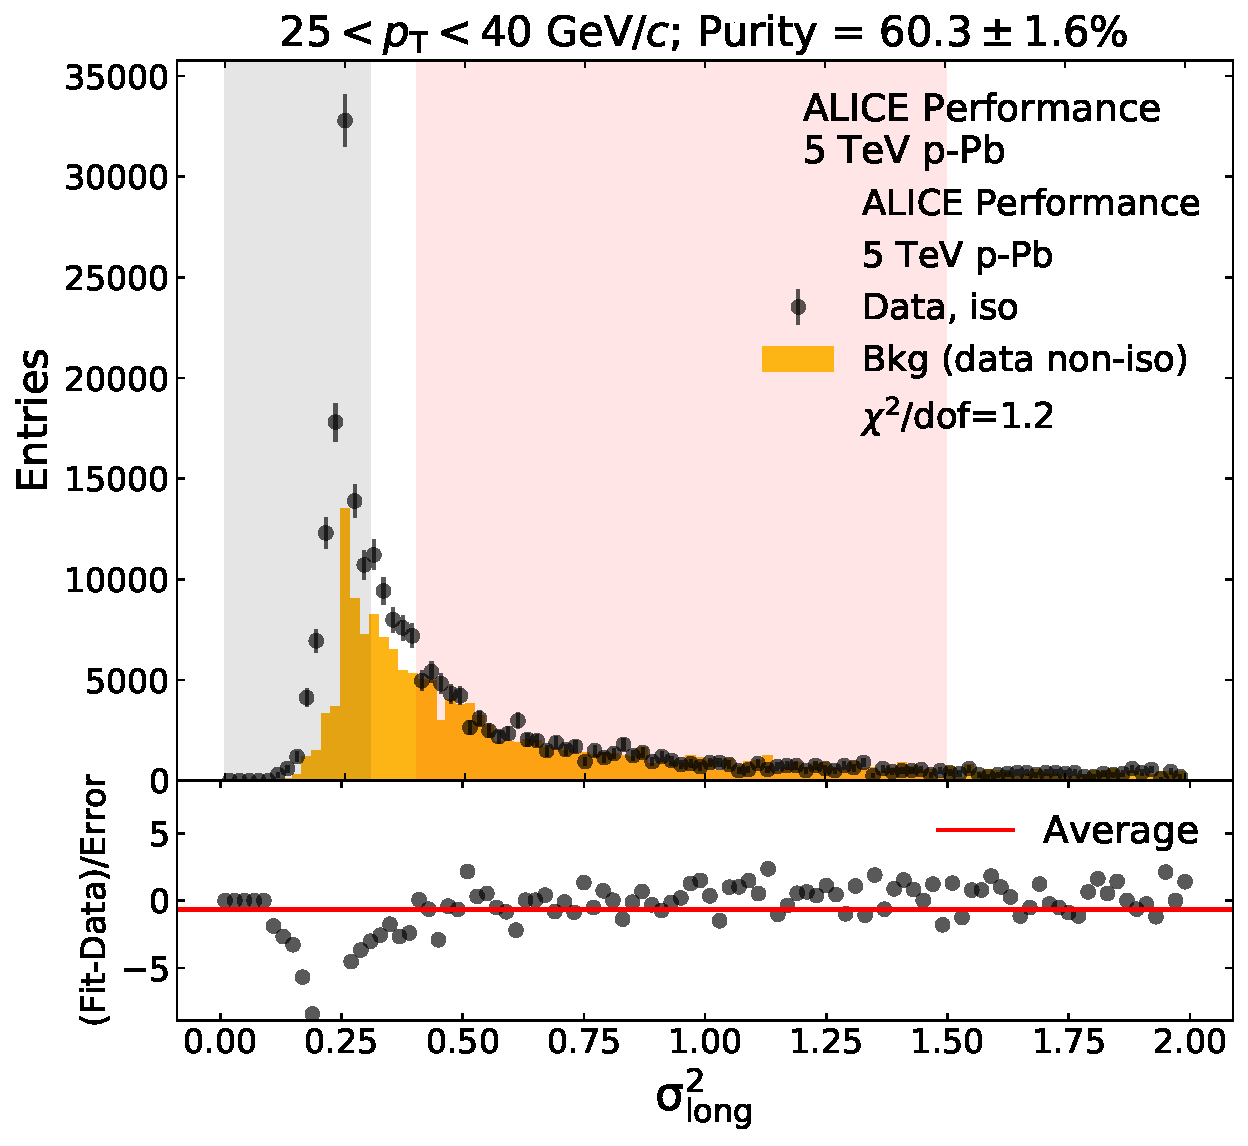
\includegraphics[width=0.38\textwidth]{Data_Analysis/Purity/bf-example-p-Pb-cluster_Lambda-25-40.pdf}
\caption{Template fit results of background-only template method for pp and \pPb~data. The yellow histograms are the predicted counts given the best-fit value of the total number of clusters in the background dominated region. The hatched gray area represents the interval considered for the purity estimate. The bottom panels show the normalized residuals of the fit, considering the statistical uncertainty on the isolated data and the background template added in quadrature. }
\label{BkgOnlyFit_pPb}
\end{figure}

This method makes the additional assumption that the fraction of signal misclassified as background is small. Strictly speaking, this method yields a lower limit on the extracted purity. The results agree with the nominal results within a few percent, indicating that the measurement is not particularly sensitive to the details of the modeling of the shower shape. As a conservative estimate, the full difference between the nominal results is taken as a systematic uncertainty in the signal template.

As an additional check, the signal template is smeared by multiplying the $\lambdasquare$ of each cluster by a random number selected from a Gaussian with a fixed width before then calculating the purity with this smeared distribution. This was done for a variety of widths up to 10\%, which is much larger than the expected MC simulation mismodelling, and was found to yield a smaller uncertainty than the background-only fit (See Appendix~\ref{sec:smearingsignaltemplate} for more details). Thus, the uncertainty estimated by the background-only fits as described in the previous paragraph is taken as a final estimate of the systematic uncertainty on the purity arising from the signal template.

\FloatBarrier
\subsection{Sideband variation in the background template}
\label{sec:bkgtemplate}
To estimate the shower-shape distribution for the $\ydecay$ background in the template fit, a sideband in the cluster isolation variable is used. Only the shape of this distribution is relevant, as the overall background normalization in the signal region (i.e. the purity) is measured with the template fit. As in any analysis using a sideband technique, nominally a sideband as close as possible to the signal region and as narrow as possible is used. Here, how the sideband region is chosen is discussed and the systematic uncertainty that arises from this arbitrary choice is addressed.

The cluster isolation distribution is divided into narrow (2 \GeVc) overlapping regions, each of which is used to estimate the background shower-shape distribution. A template fit is performed with each distribution and the $\chi^2$/dof and purity are calculated for each fit and plotted as a function of the anti-isolation region used to create the background template in Figure~\ref{sidebandslices}. Then, the $\chi^2$/dof distribution is examined to determine which regions of anti-isolation result in good fits in the template fit procedure: 5--10 \GeVc~is chosen to be the sideband definition in the final purity calculation.

To calculate the systematic uncertainty on the purity due to this selection, the full range of purities reached by the narrow bands of anti-isolation that fall within 5--10 \GeVc~is considered. Converting the full extent to a systematic uncertainty is a matter of dividing by $\sqrt{12}$ (i.e, the 1 $\sigma$ for a uniform distribution). This results in an absolute uncertainty on the purity of 0.7--5.8$\%$, depending on the collision system and cluster \pt~range.

\begin{figure}[htpb]
\center
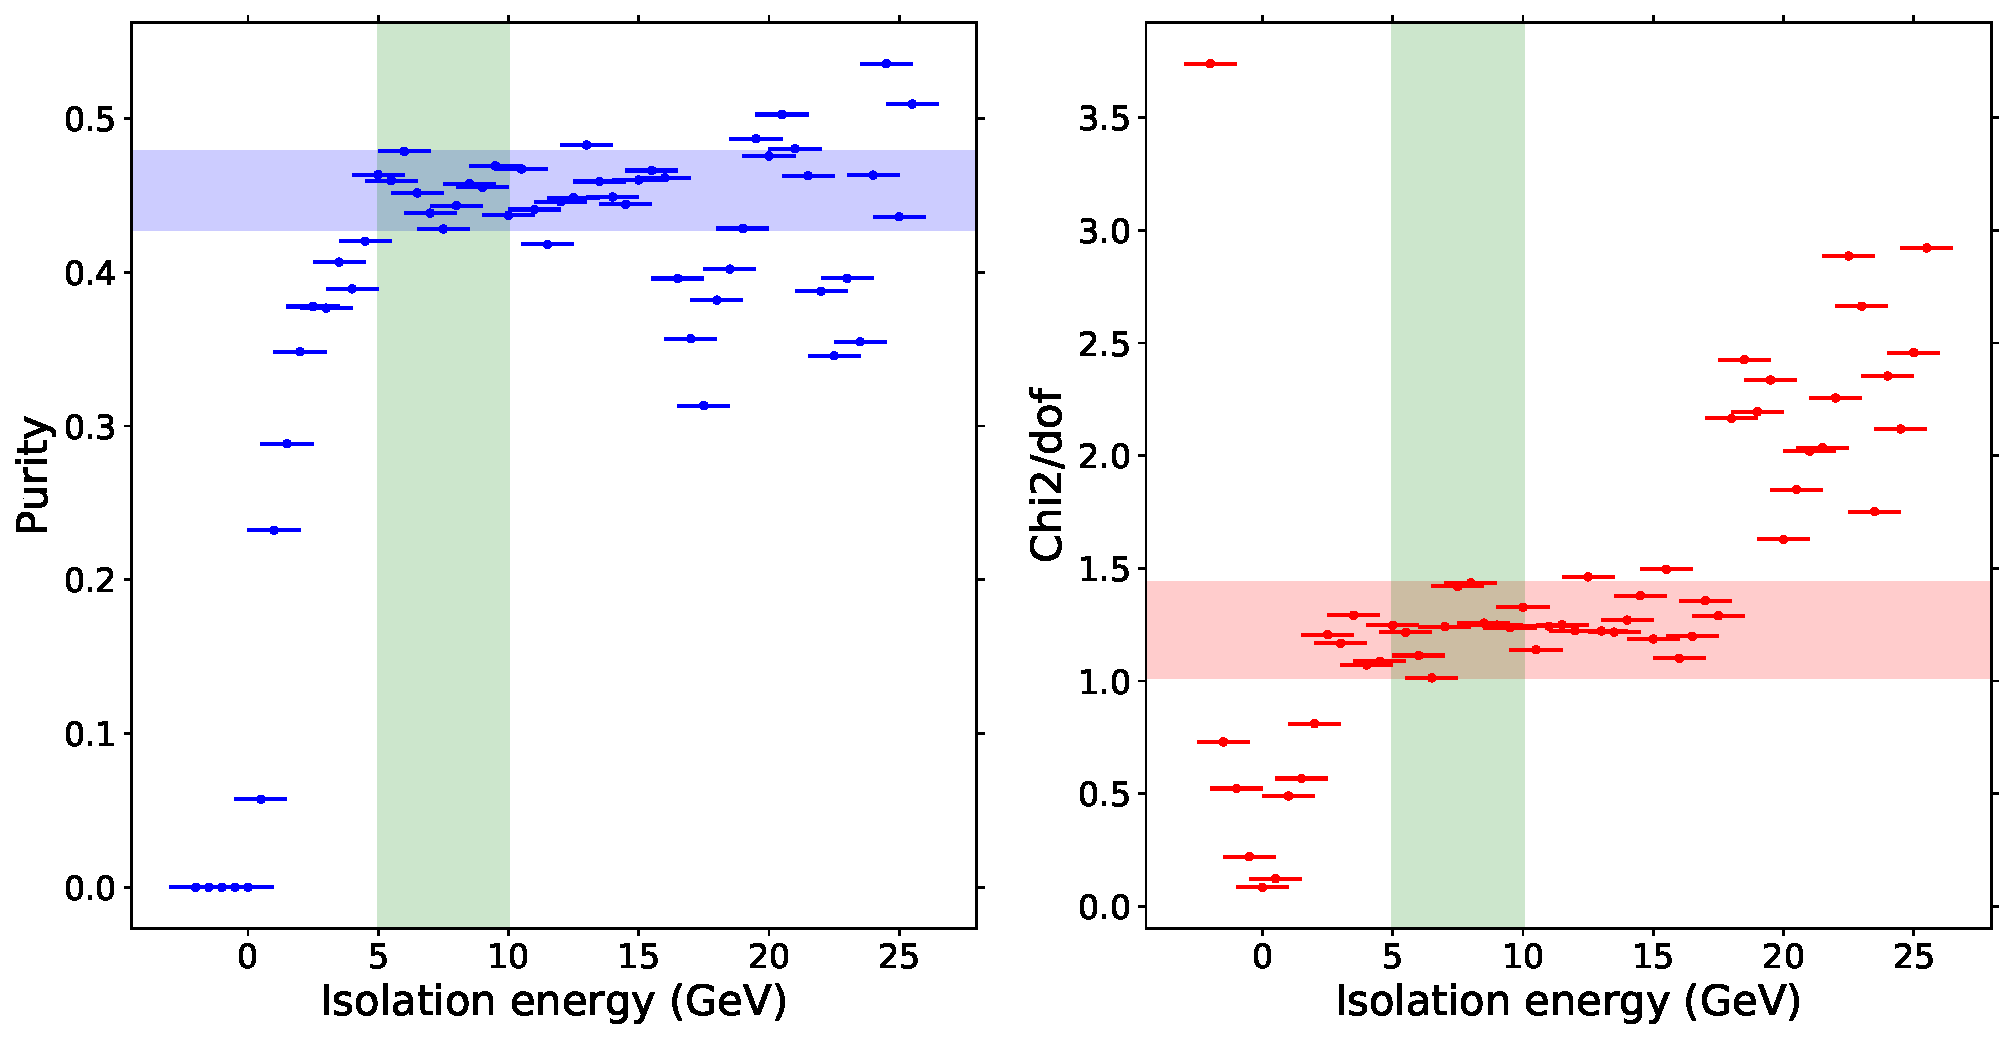
\includegraphics[width=1.0\textwidth]{Data_Analysis/Purity/antiiso-selection-pp-cluster_Lambda-15-20.pdf}\\
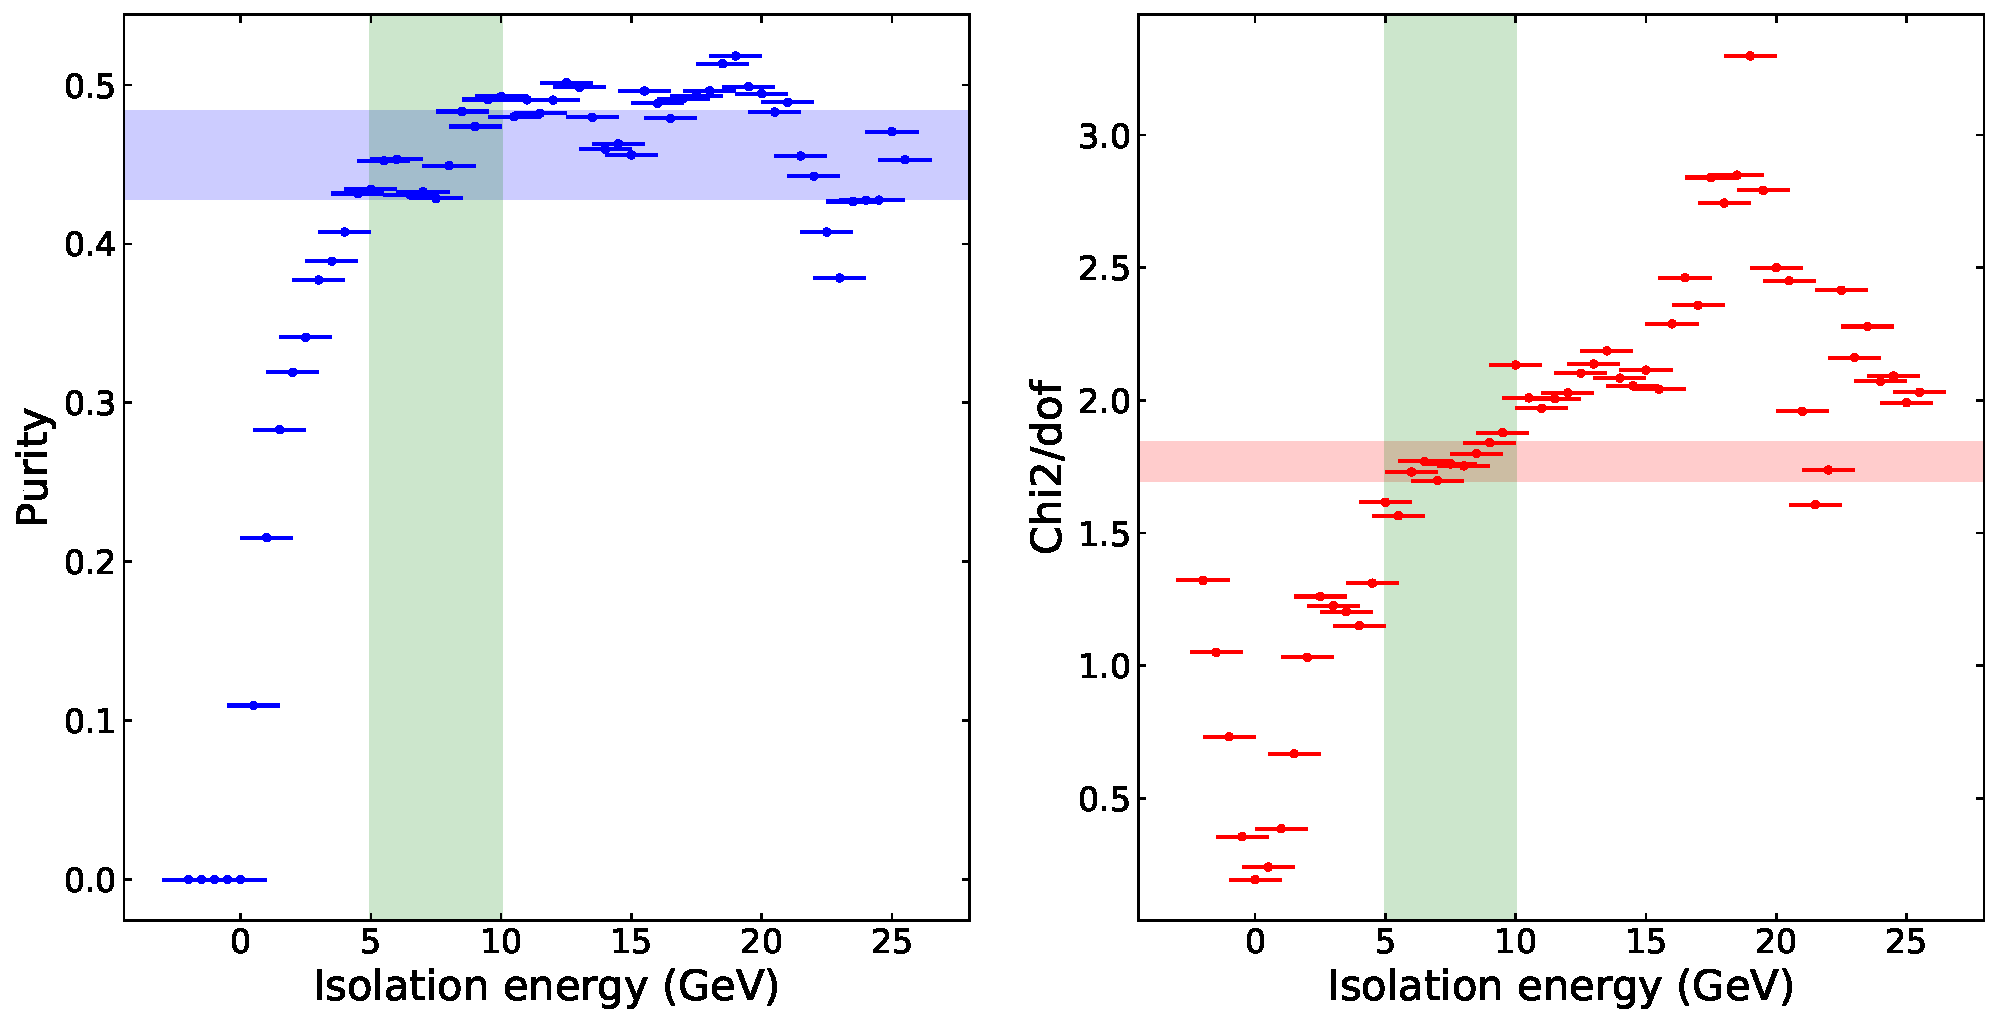
\includegraphics[width=1.0\textwidth]{Data_Analysis/Purity/antiiso-selection-p-Pb-cluster_Lambda-15-20.pdf}
\caption{Template fit results (purity and $\chi^2$/dof) as a function of anti-isolation region for clusters with $15 < \pt < 20$ \GeVc~in pp (top) and \pPb~(bottom). The green band shows the selected sideband region. The blue and red bands show the full extent of the purity within the selected sideband region.}
\label{sidebandslices}
\end{figure}

\subsection{Background template correction}
\label{sec:bkgtemplatecorrection}
Due to the correlation between the isolation and shower shape, the template extracted from the anti-isolated sideband does not exactly reflect the shape of the background in the signal region. Clusters in the isolation sideband have more associated activity than those in the true isolated background and thus emphasize the non-signal region of the shower-shape distribution. Consequently, using the isolation sideband instead of the true isolated background yields systematically higher purities. It should be noted that a similar observation was made for example by the CMS collaboration in their template-fit purity measurements (e.g. Ref.~\cite{Sirunyan:2017qhf})

A dijet MC simulation is used to correct this bias, as described in Equation~\ref{eq:bkgtemplatecorrection}. However, this correction is only valid to the extent that the dijet MC reproduces the data. To estimate the systematic uncertainty on this correction, a technique based on a method used in the ABCD calculation~\cite{Erwann} is implemented. In particular, a double ratio is used to check to which extend does the dijet MC describe the background-dominated region in data: 

\begin{equation}
    \text{Double ratio} = \frac{\text{Iso}_{\text{data}}/\text{Anti-iso}_{\text{data}}}{\text{Iso}_{\text{MC}}/\text{Anti-iso}_{\text{MC}}}
    \label{eq:bkgtemplatedoubleratio}
\end{equation}

In the signal region of the shower shape distribution (0.0--0.3 for $\lambdasquare$), this double ratio will be far from unity, as the data have prompt photons and the dijet MC do not. However, away from that region, where background dominates, the double ratio should be flat (i.e. have no slope) if the dijet MC reproduces the background shower-shape of the data. It should be noted that for this analysis, only the shape is important and overall normalization is irrelevant. At a minimum, the variation in the double ratio is expected to be smooth. Thus the double ratio is fit to smooth functions (linear and exponential) in a shower shape range away from the signal region and extrapolate the fit back into the signal region. A similar procedure was used isolated-photon purity measurements with the ABCD method~\cite{Acharya:2019jkx}.

Fits to the double ratio are shown in Figures~\ref{fig:bkgtemplatedoubleratiofits_pp} and~\ref{fig:bkgtemplatedoubleratiofits_pPb}, for pp and \pPb~data respectively. It was found that the linear and exponential fits gave nearly identical results. In particular, the slope was sufficiently small that the higher-order terms in the exponential were negligible. Thus for the purposes of estimating the systematic uncertainty due to the background template correction, only linear fits to the double ratio were done. In order to remove covariance effects between the slope and intercept, the fits were forced to go through the weighted average of the double ratio value within the fit range at the center of the fit range, making it a single-parameter linear fit with only the slope as a free parameter. This allowed us to propagate the fit uncertainty on the slope to an uncertainty on the purity.


\begin{figure}[htpb]
    \centering
    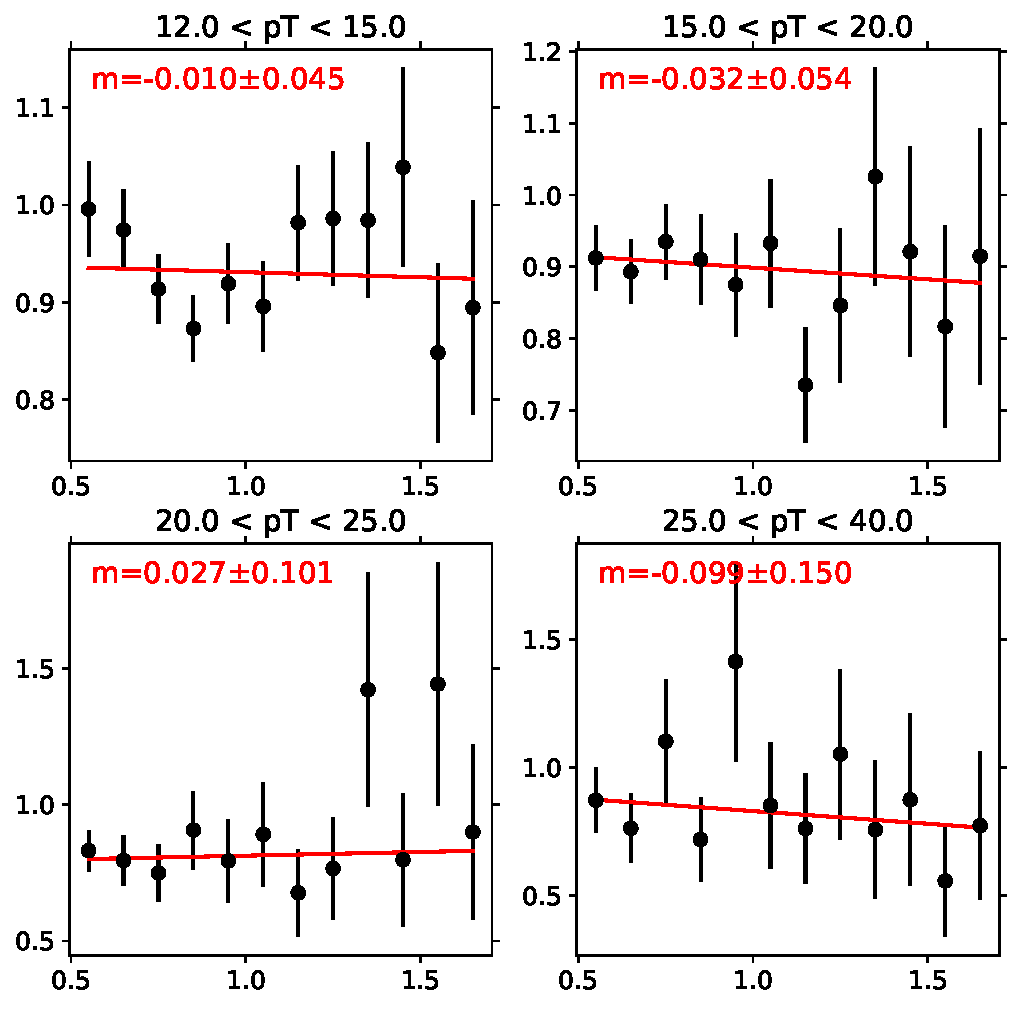
\includegraphics[width=\textwidth]{Data_Analysis/Purity/single-linear-fits-pp}
    \caption{Linear fits for the double ratio (as described in Equation~\ref{eq:bkgtemplatedoubleratio}) for the $\lambdasquare$ variable in pp data.  Included are the value and uncertainty of the fitted slope (in red).}
    \label{fig:bkgtemplatedoubleratiofits_pp}
\end{figure}


\begin{figure}[htpb]
    \centering
    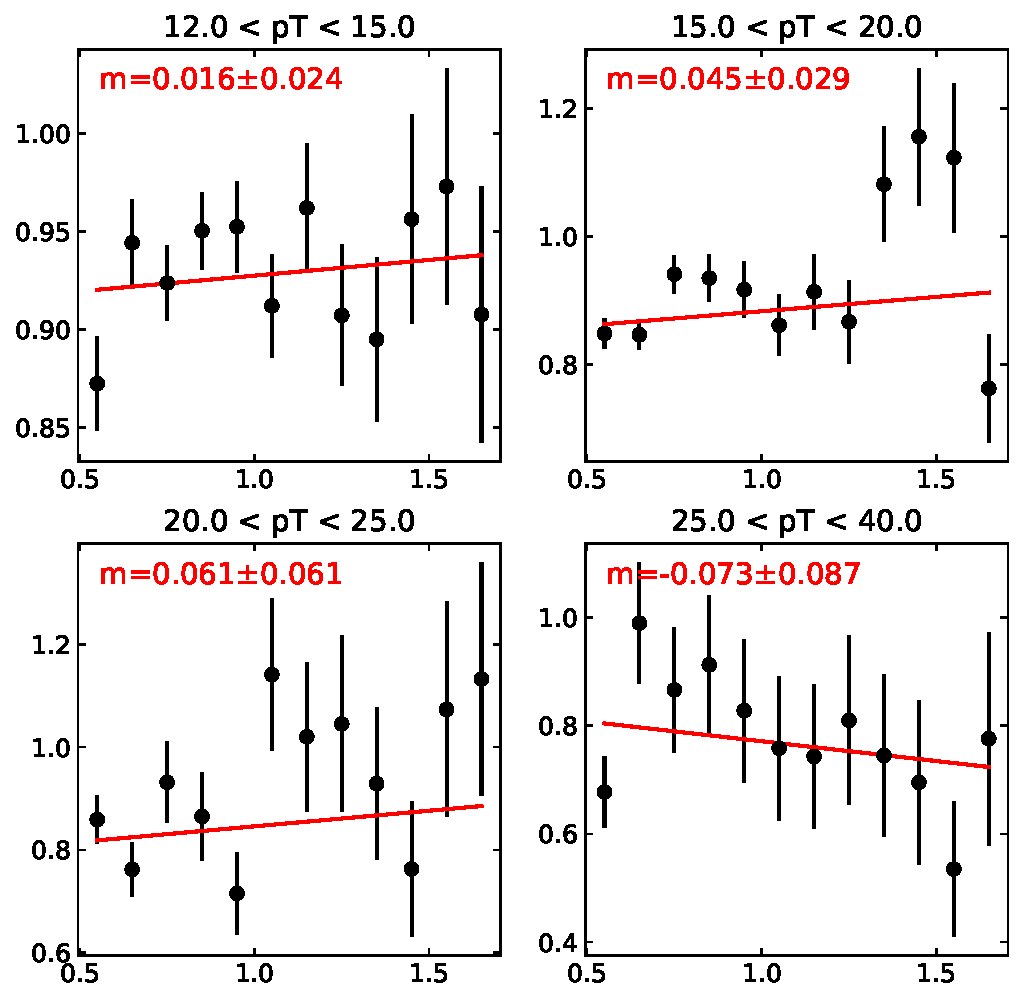
\includegraphics[width=\textwidth]{Data_Analysis/Purity/single-linear-fits-p-Pb}
    \caption{Linear fits for the double ratio (as described in Equation~\ref{eq:bkgtemplatedoubleratio}) for the $\lambdasquare$ variable in \pPb~data.  Included are the value and uncertainty of the fitted slope (in red).}
    \label{fig:bkgtemplatedoubleratiofits_pPb}
\end{figure}

These linear fits to the double ratio were done in two fit ranges: 0.5--1.5 and 0.5--1.75 for $\lambdasquare$. In all cases, it was found that the slopes were consistent with 0 within the fit uncertainties and thus concluded that that the dijet MC was consistent with the data. Therefore, an additional double-ratio correction is not applied to the Weights function in Equation~\ref{eq:bkgtemplatecorrection}. It was also found that the double ratio fits with the different fit ranges gave purities consistent with each other. So in order to minimize the amount of extrapolation, the fit in the largest reasonable fit ranges for each of the variables was done (the larger of each of the ranges described at the beginning of this paragraph). 

The uncertainty on that double ratio fit is then taken and propagated to a purity uncertainty. This purity uncertainty was then taken to be the systematic uncertainty on the background correction. It varies between 1.2--3.4\% (absolute) depending on cluster \pt~and collision system.


\FloatBarrier
%%%%%%%%%%%%%%%%%%%%%%%%%%%%%%%%%%%%%%%%%%%%%%%%%%%%%%%%%
\subsection{Summary of Systematic Uncertainties on Purity Measurement}

Tables~\ref{tab:pursystppblambda} and~\ref{tab:pursystpplambda} give the full estimates of the systematic uncertainties in both collision systems. No single source of systematic uncertainty dominates across \pt~ranges or collision systems.


\begin{table}[htpb]
    \centering
        \caption{Summary of the systematic uncertainties on the purity as measured with $\lambdasquare$ in \pPb~collisions. All values are in absolute percentage. ``Stat.'' refers to the statistical uncertainty; ``Signal'' refers to the signal template uncertainty; ``Anti-iso'' refers to the uncertainty due to the sideband selection; ``Bkg'' refers to the uncertainty due to the background template correction; ``Total'' is the sum of the previous three columns in quadrature.}
    \begin{tabular*}{1.0\columnwidth}{@{\extracolsep{\fill}}lcccccc@{}}
    \hline
    	pT(GeV/$c$) & Purity & Stat. & Signal & Anti-iso & Bkg & Total syst \\ \hline
    	12.0-15.0 & 20.7 & 1.1 & 1.1 & 0.8 & 1.5 & 2.0 \\
    	15.0-20.0 & 34.2 & 1.2 & 2.0 & 1.6 & 1.2 & 2.8 \\
    	20.0-25.0 & 47.6 & 1.7 & 1.9 & 1.1 & 1.7 & 2.7 \\
    	25.0-40.0 & 54.6 & 1.8 & 2.3 & 2.4 & 2.1 & 3.9 \\
    \end{tabular*}
    \label{tab:pursystppblambda}
\end{table}


\begin{table}[htpb]
    \centering
        \caption{Summary of the systematic uncertainties on the purity as measured with $\lambdasquare$ in pp collisions. All values are in absolute percentage. ``Stat.'' refers to the statistical uncertainty; ``Signal'' refers to the signal template uncertainty; ``Anti-iso'' refers to the uncertainty due to the sideband selection; ``Bkg'' refers to the uncertainty due to the background template correction; ``Total'' is the sum of the previous three columns in quadrature.}
    \begin{tabular*}{1.0\columnwidth}{@{\extracolsep{\fill}}lcccccc@{}}
    \hline
    	pT(GeV/$c$) & Purity & Stat. & Signal & Anti-iso & Bkg & Total syst \\ \hline
    	12.0-15.0 & 20.1 & 1.7 & 2.0 & 1.2 & 2.9 & 3.7 \\
    	15.0-20.0 & 31.7 & 2.0 & 2.5 & 1.5 & 2.4 & 3.8 \\
    	20.0-25.0 & 47.3 & 2.9 & 0.8 & 3.0 & 2.8 & 4.2 \\
    	25.0-40.0 & 48.5 & 3.5 & 5.9 & 4.0 & 3.4 & 7.9 \\
    \end{tabular*}
    \label{tab:pursystpplambda}
\end{table}


%\subsection{Isolation and Shower shape correlation}

%\subsection{EMCal Acceptance Variation}

%\subsection{Purity variation (Last minute IRC check)}

%\subsection{Check on Isolation Criterium within EMCal Acceptance}
%\label{sec:iso_acceptance_check}

\section{Tracking}
\subsection{Comparison to Published Data}
\label{sec:tracking_published_comparision}
In this section results of the closure test, which is described in Section~\ref{sec:closurewithdata}, are show with the goal to validate the MC simulation description of track efficiency, fake rate and momentum smearing corrections using the published data. 

Figure~\ref{fig:RefoldedComparisonSpectra} shows the correction procedure on published data at various stages: the pink line is the published charged-particle spectrum in \pPb~collisions at {$\sqrt{s_{\mathrm{NN}}}=$ 5 TeV} from Ref.~\cite{Acharya:2018qsh}; the red line is the published data spectra after multiplying by the efficiency; the orange line is the red spectrum multiplied by the response matrix according to Equation~\ref{eq:refold_eq}:

\begin{equation}\label{eq:refold_eq}
R_{j} = \Sigma M_{ij} \cdot P_{i}
\end{equation}
where $M$ is the response matrix, $P$ is the published data times the efficiency, $R$ is smeared $\pt$ spectrum. The smeared $\pt$ spectrum should be consistent with the measured spectrum after removal of the fake-track contribution.

A ''folding'' of the published spectra is shown instead of an ''unfolding'' of the measured spectra because the former is a unique transformation and avoids the need for systematic studies on the stability of the unfolding procedure. This allows us to focus on unambiguously testing the response matrix. 

\begin{figure}[htpb]
\centering
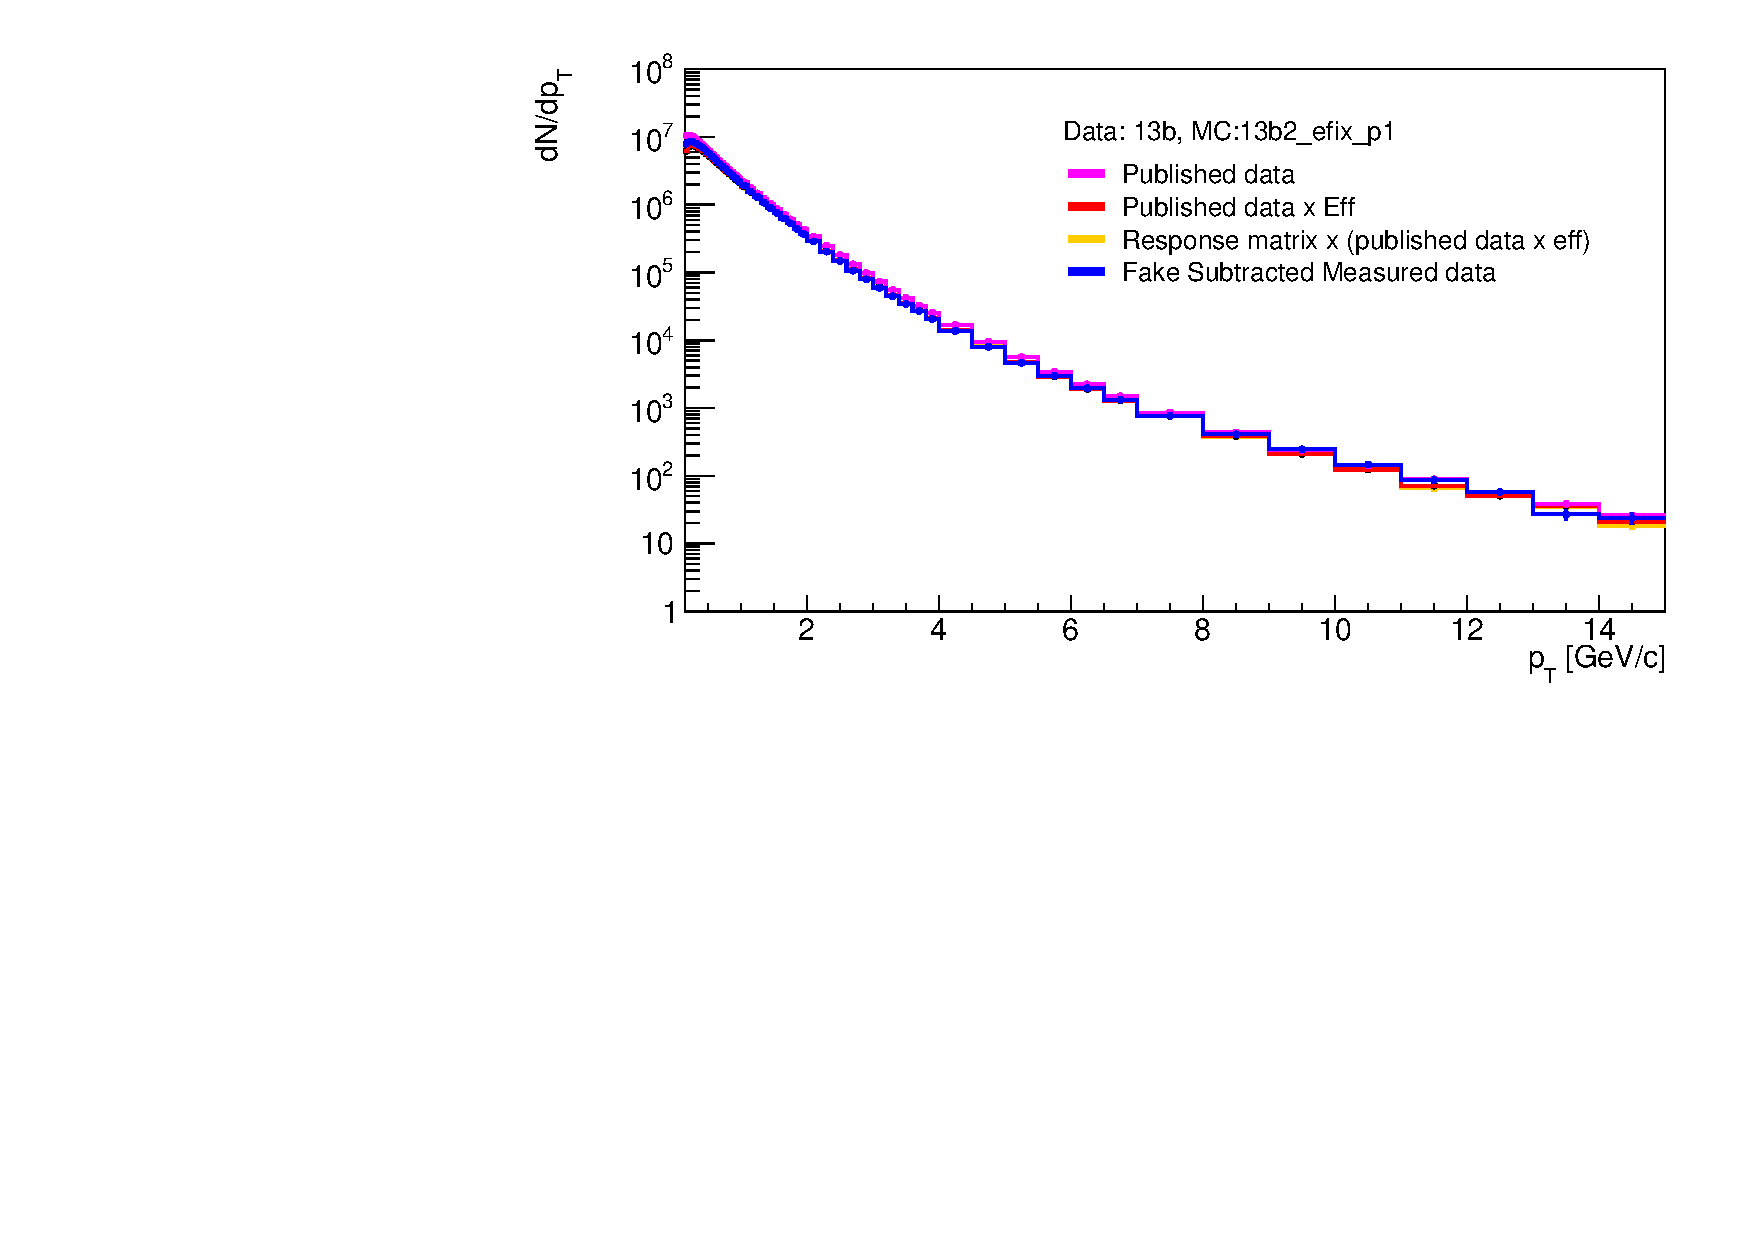
\includegraphics[width=.95\textwidth]{Data_Analysis/Tracking/refolding_pPb_tpc_MBMC_0GeV15GeV_dNdpt.pdf}
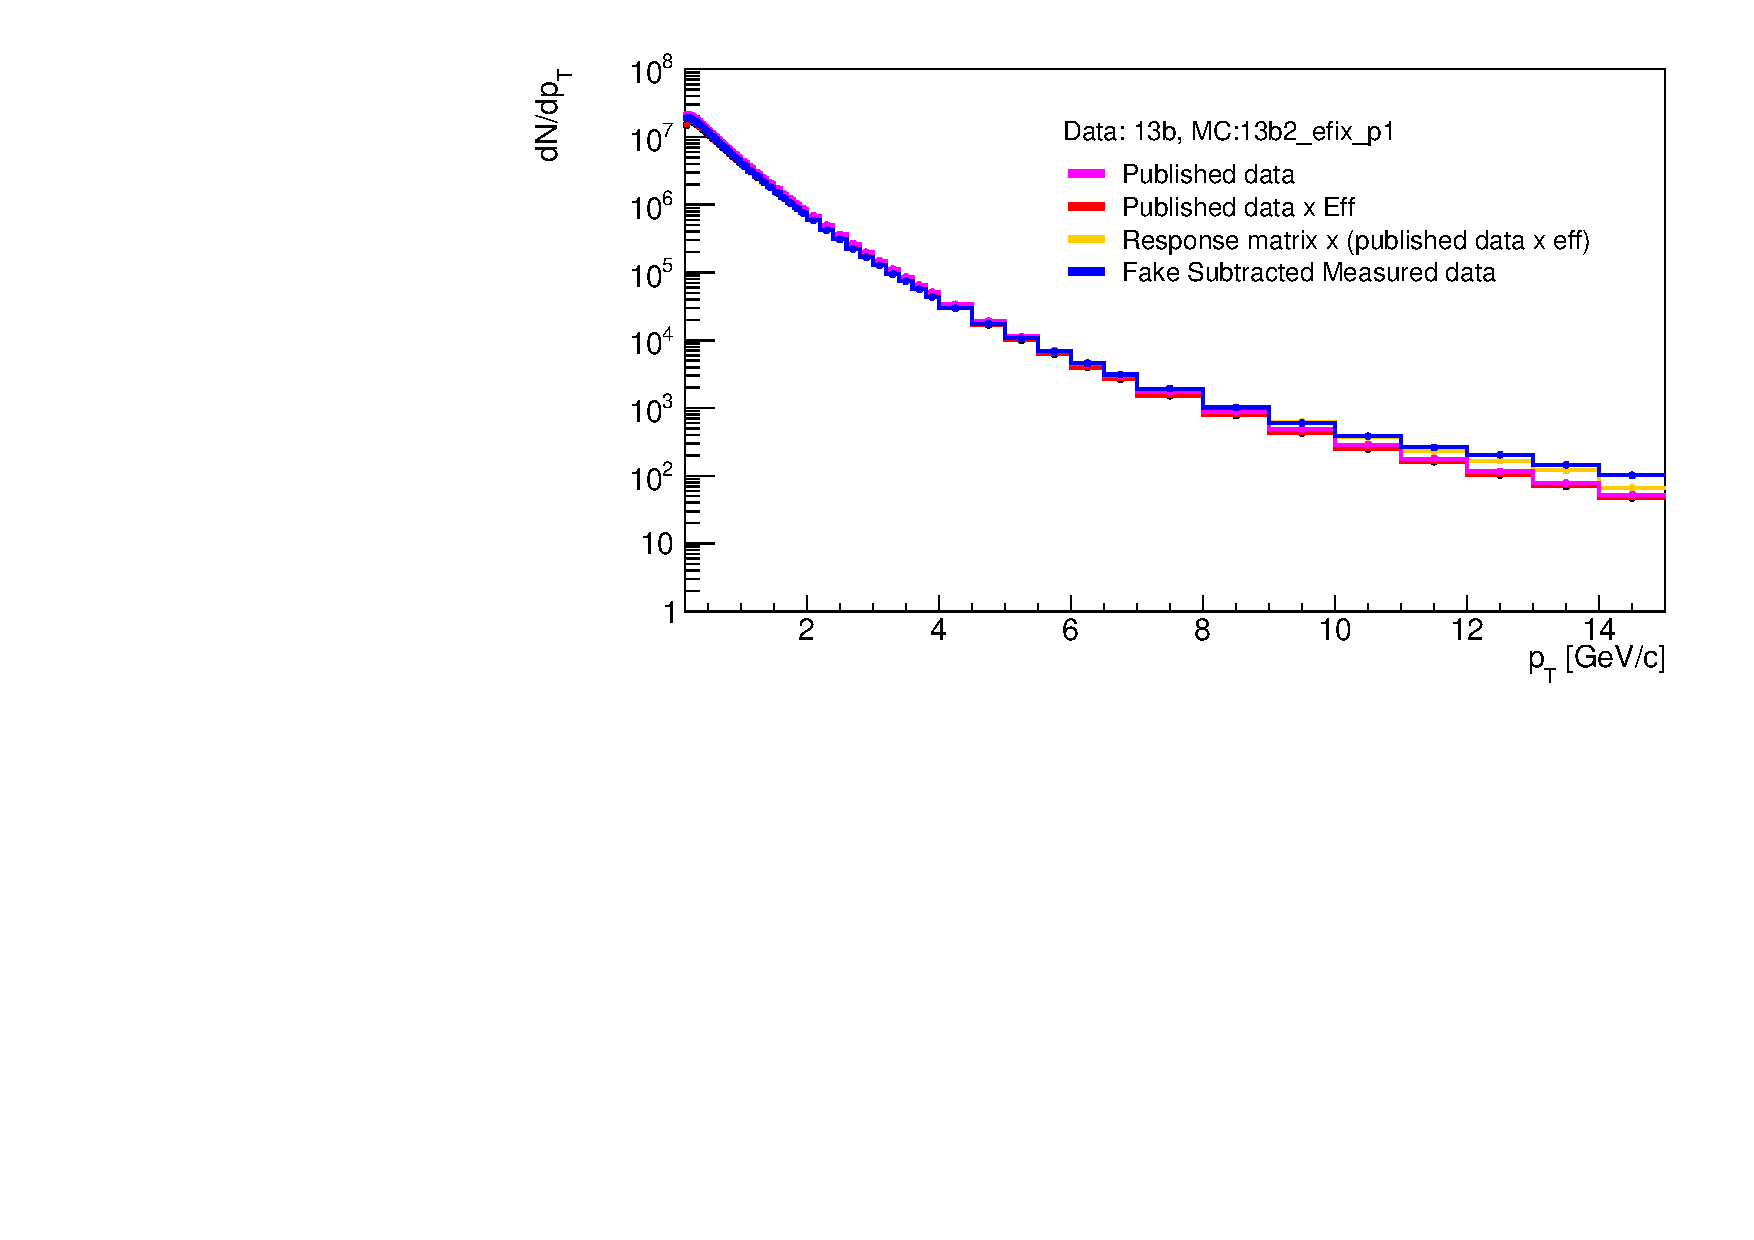
\includegraphics[width=.95\textwidth]{Data_Analysis/Tracking/refolding_pPb_its_MBMC_0GeV15GeV_dNdpt.pdf}
\caption{Smearing of published data at various stages, using TPC+ITS (top) and ITS only (bottom) response matrices. The pink is the published data \pt~spectrum. The red is after the pink has been multiplied by the efficiency. The orange is the spectra after applying the response matrix in order to induce the smearing on the red. The blue is fake-rate-subtracted measured data.}
\label{fig:RefoldedComparisonSpectra}
\end{figure}

The published data has a total uncertainty (quadrature sum of statistical and systematic uncertainties) that ranges from $1.8\%$ at 1 \GeVc, reaches $4.8\%$ by 10 \GeVc~and grows quickly to about 20$\%$ at 15 \GeVc, where it is dominated by the statistical uncertainty. 

Figure~\ref{fig:RefoldedComparison} shows the ratio of the measured fake-subtracted spectrum and the smeared published spectra. The ratio of the published data to the smeared published data is shown to illustrate the impact of the momentum smearing, which is less than a $2\%$ effect for TPC+ITS tracks but it reaches up to a factor of two in the ITS-only case. The closure-test ratios from TPC+ITS tracking are consistent with unity within uncertainties, which is expected. The more interesting result is that the ratios due to ITS-only tracking are within $\pm$5\% of unity in the range between 0.85--10 \GeVc and within $\pm$8\% of unity in the range between 0.5--0.85 \GeVc, shown by the dashed lines in the bottom plot of Figure~\ref{fig:RefoldedComparison}, which is the range used for the $\gammaiso$--hadron analysis. This difference from unity is used as a systematic uncertainty on the tracking.

\begin{figure}[htpb]
\center
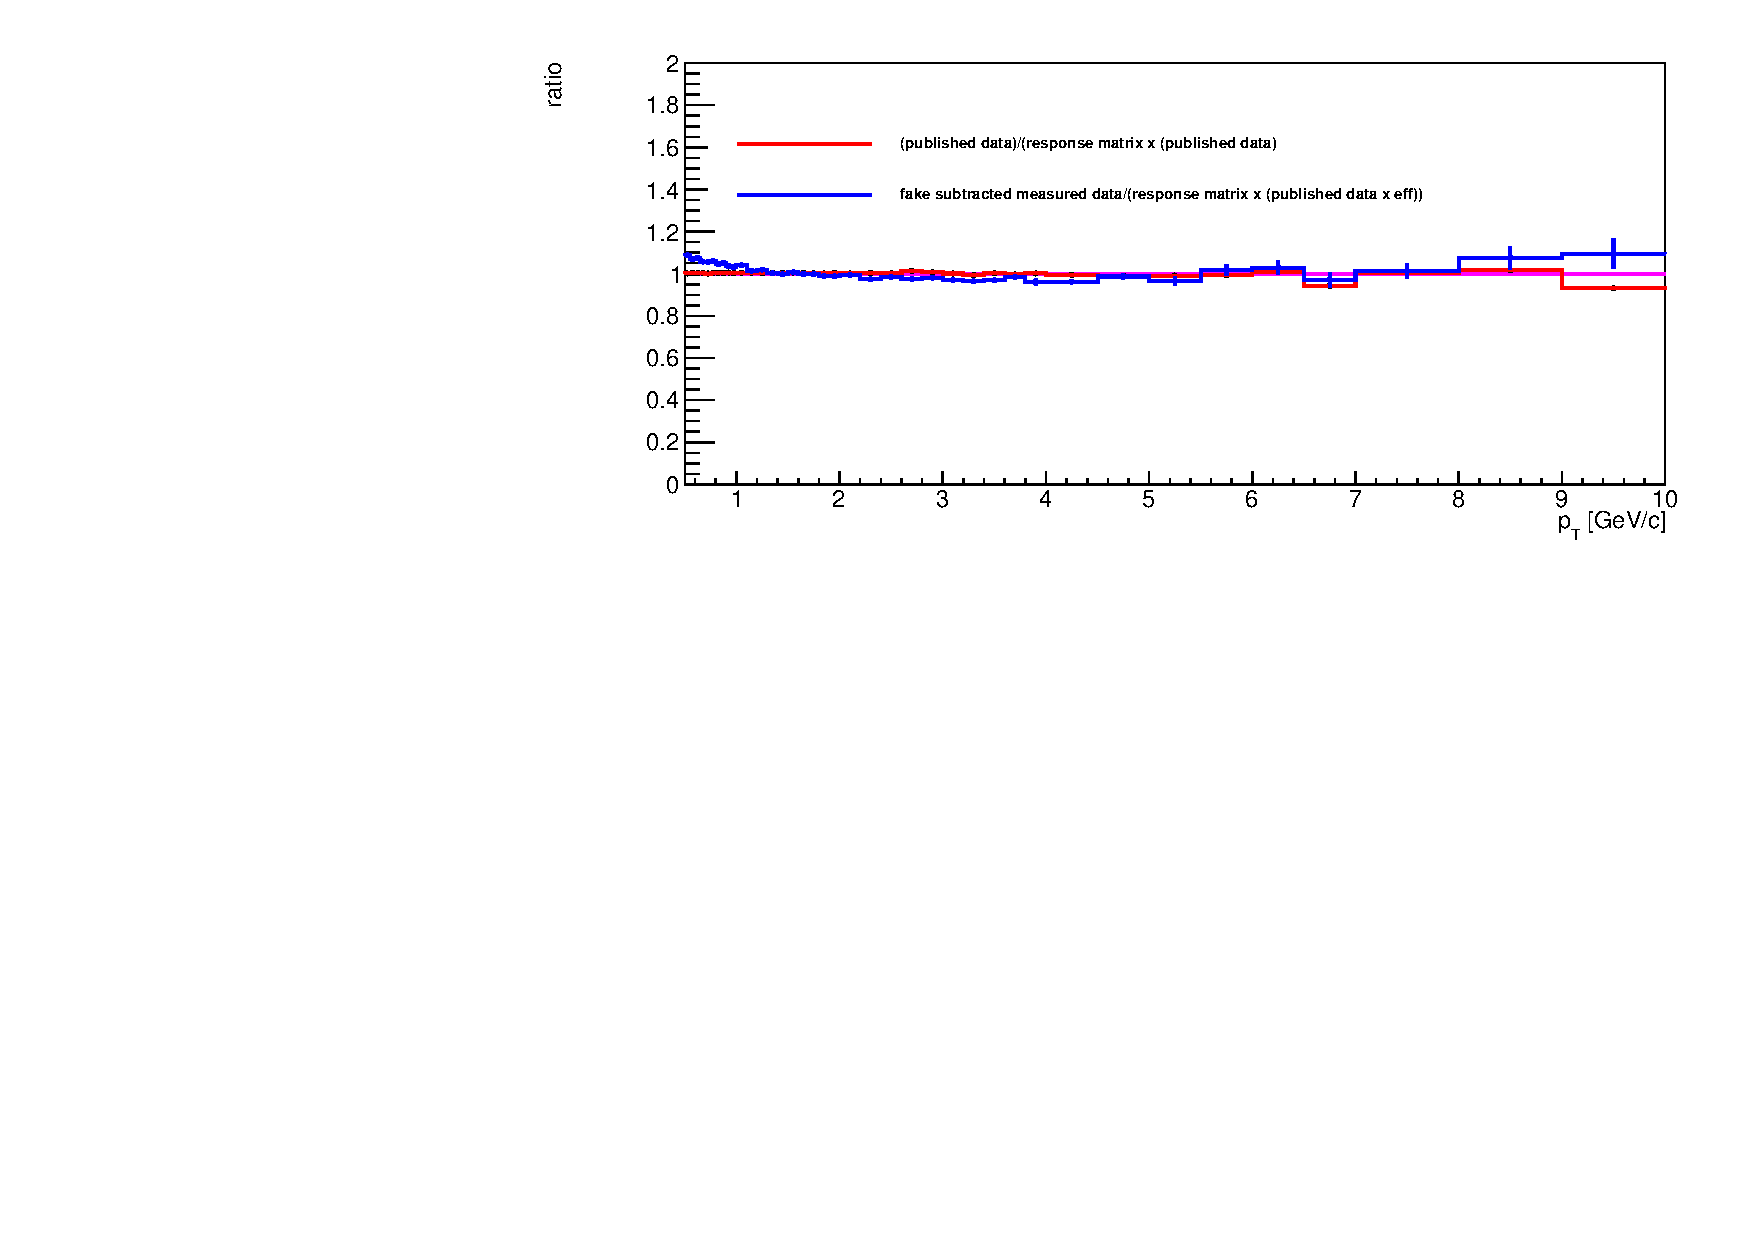
\includegraphics[width=.95\textwidth]{Data_Analysis/Tracking/ratio_refolding_pPb_tpc_MBMC_1GeV15GeV_errors.pdf}
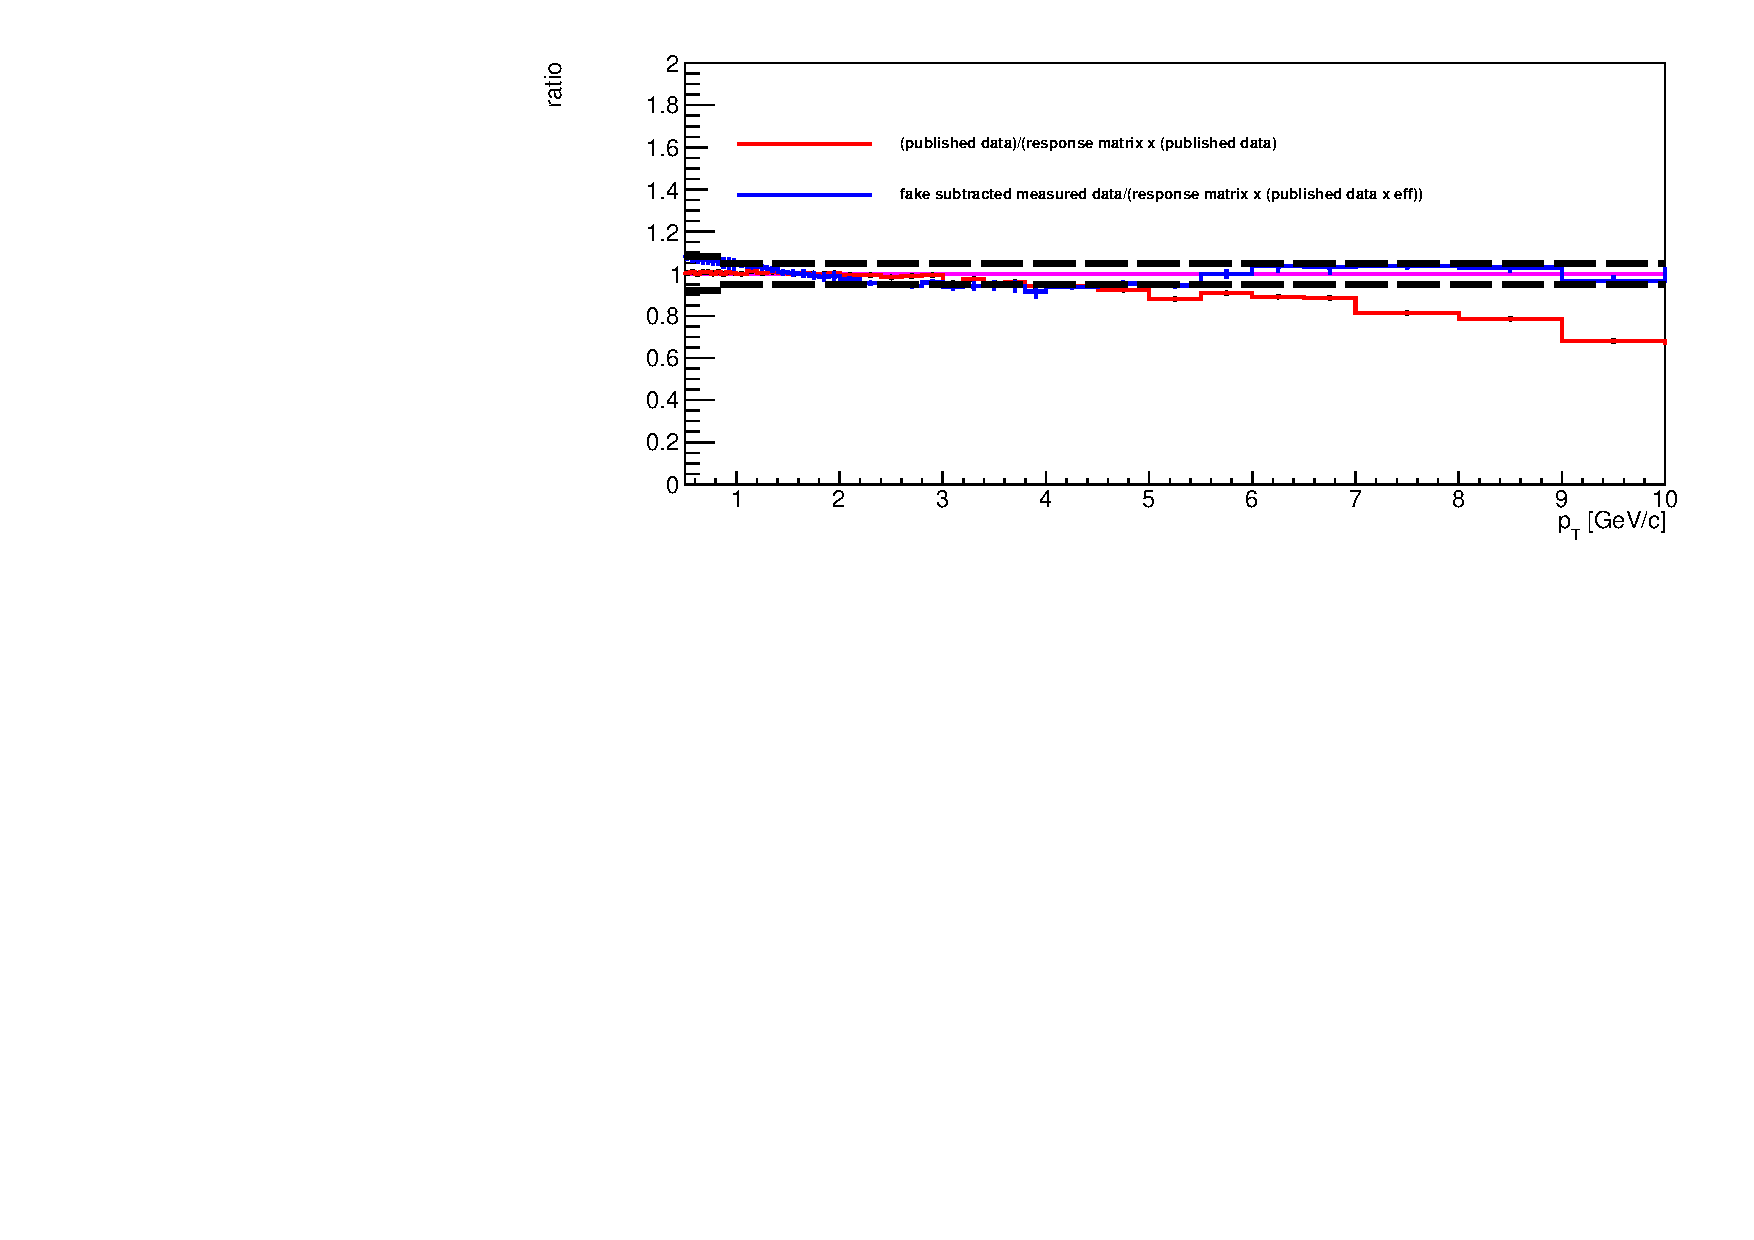
\includegraphics[width=.95\textwidth]{Data_Analysis/Tracking/ratio_refolding_pPb_its_MBMC_0GeV15GeV_errors_band.pdf}
\caption{Result of closure test comparing measured data and published data, for TPC+ITS tracking (top) and ITS-only tracking (bottom). The red curves show the ratio of the reference spectra to the smeared reference spectra. The blue curves show the ratio of the fake-subtracted measured data and the smeared reference spectra. Ideally the blue curve would be flat at unity. The error bar represents statistical uncertainty only for the blue curve, and the quadrature sum of statistical and systematic uncertainties for the red curve. Additionally, the dashed lines from 0.5 to 0.85 \GeVc represent an 8\% band around 1, while the dashed lines from 0.85 to 10.0 \GeVc represent a 5\% band around 1.}
\label{fig:RefoldedComparison}
\end{figure}

The statistically-significant deviation from the published data with ITS-only tracking at high $\pt$ (blue curve in lower panel of Figure~\ref{fig:RefoldedComparison}), could be due to several reasons  including improper modeling of a rapid deterioration of the momentum resolution and underestimation of fake rate. Further work would be needed to understand and correct these and other effects at high $\pt$, but that lies beyond the scope of this work. 

It should be noted that these spectra are normalized per-minimum bias event and not by integral, so the fact that the ratios are close to unity reflect the fact that the efficiency calculations shown in Figure~\ref{fig:tpcEff} are an accurate description of the detector response. Based on the results shown in this section, the $\pt$ range is restricted to no more than 10 \GeVc, which is beyond the limit of the statistical power of the $\gammaiso$-hadron analysis.

\subsection{Validation of $\varphi$-dependence of efficiency}
\label{sec:phicheck}

In order to validate the description of the ITS-only tracking holes, a test with minimum-bias data is done. Apart from the effect of $\varphi$-dependent holes, the measured azimuthal angle distribution of tracks is expected to be uniform in minimum-bias data. Thus the track $\varphi$ spectrum is measured and then corrected for the $\varphi$-dependent efficiency and checked whether the distribution is flat. The level of flatness gives us a sense of the systematic uncertainties associated with mis-modeling of the $\varphi$-dependent efficiency.

Figure~\ref{fig:phiEff} shows the $\varphi$-dependence of the tracking efficiency for TPC+ITS and ITS-only tracks. The efficiency is calculated using Equation~\ref{eq:eff}, but as a function of $\varphi^{true}$ instead of \pt~$^{true}$. The TPC+ITS tracking efficiency is flat in $\varphi$ as expected, but there are dips in the efficiency for the ITS-only tracking due to dead staves in the ITS. These have little impact on the TPC+ITS tracks because the selection does not have the strict requirement on the number of ITS hits, $N_{\mathrm{ITS}} \geq$ 4, that is applied for ITS-only tracks. 

\begin{figure}[htpb]
\center
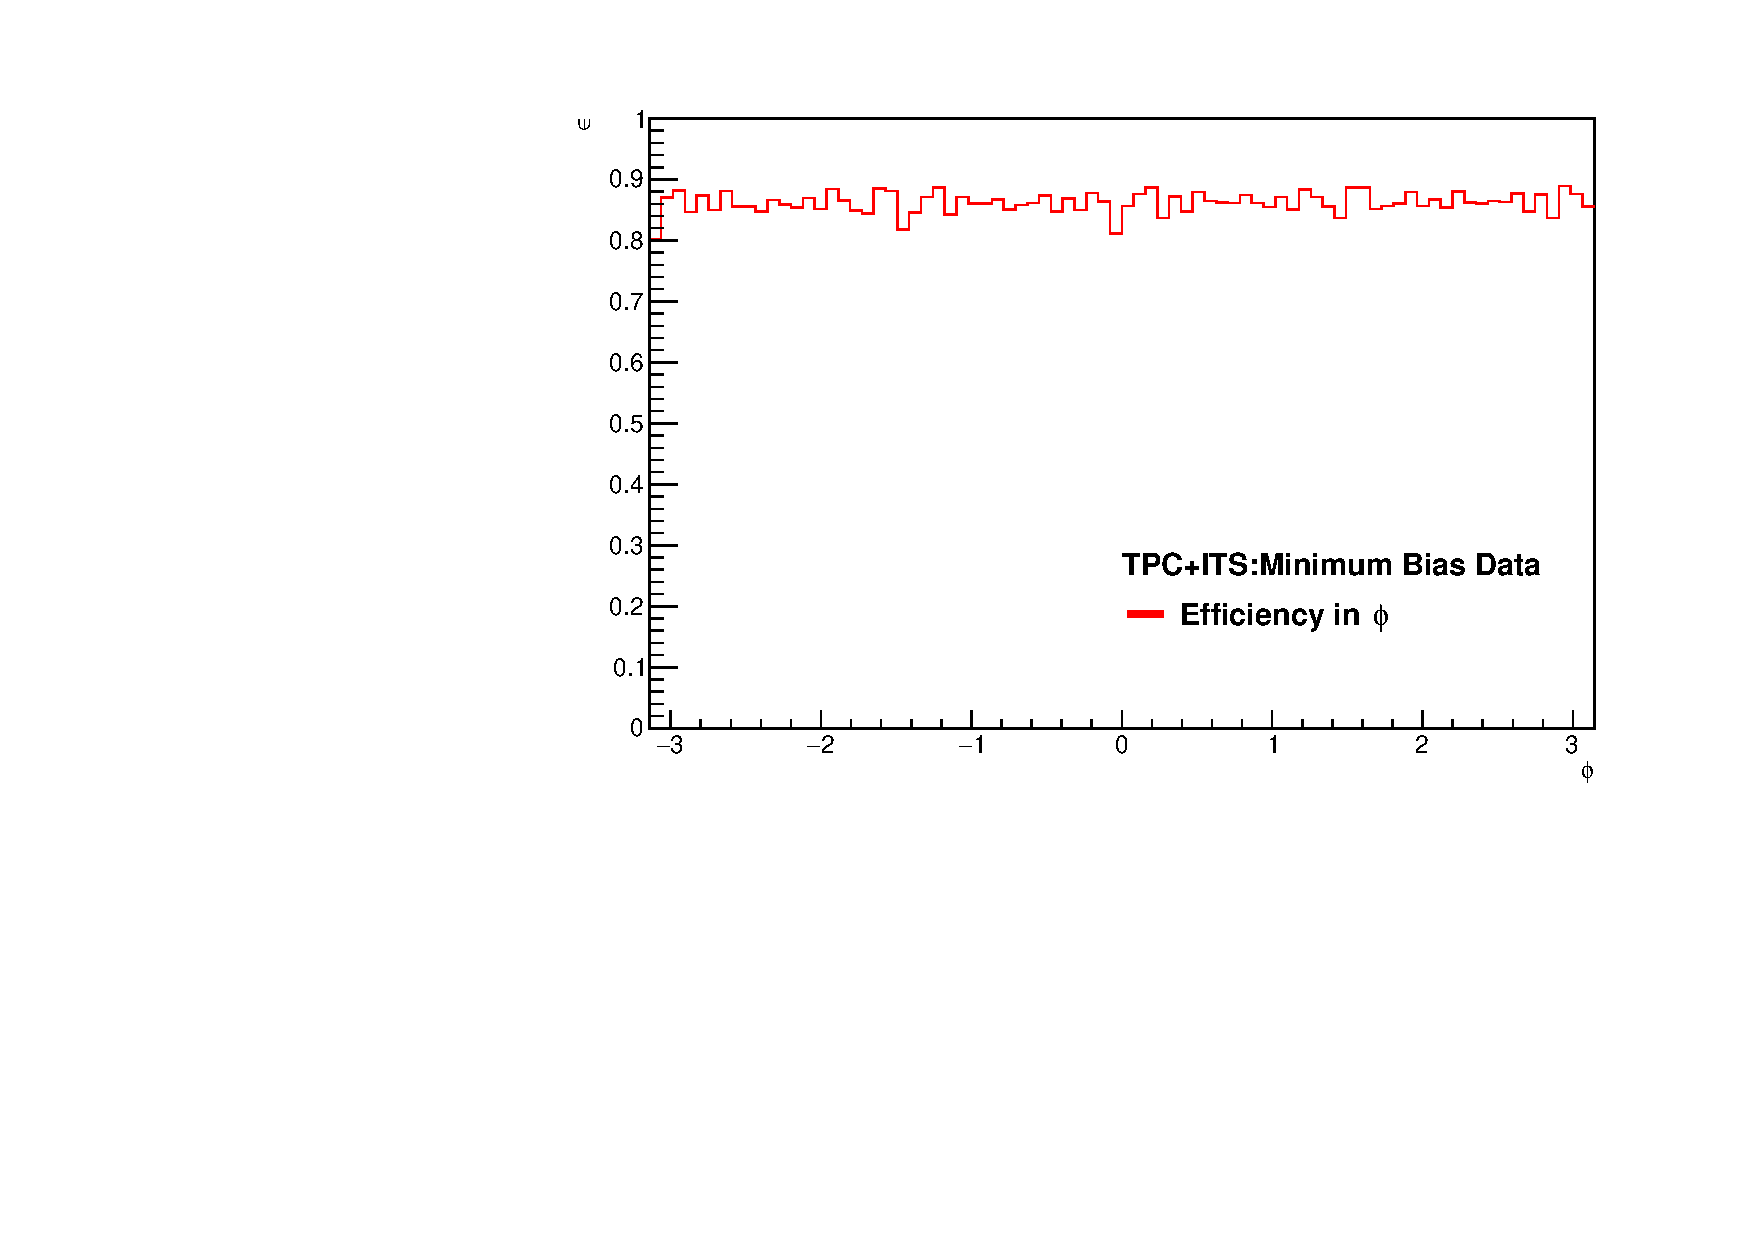
\includegraphics[width=.495\textwidth]{Data_Analysis/Tracking/tpc_phi_eff.pdf}
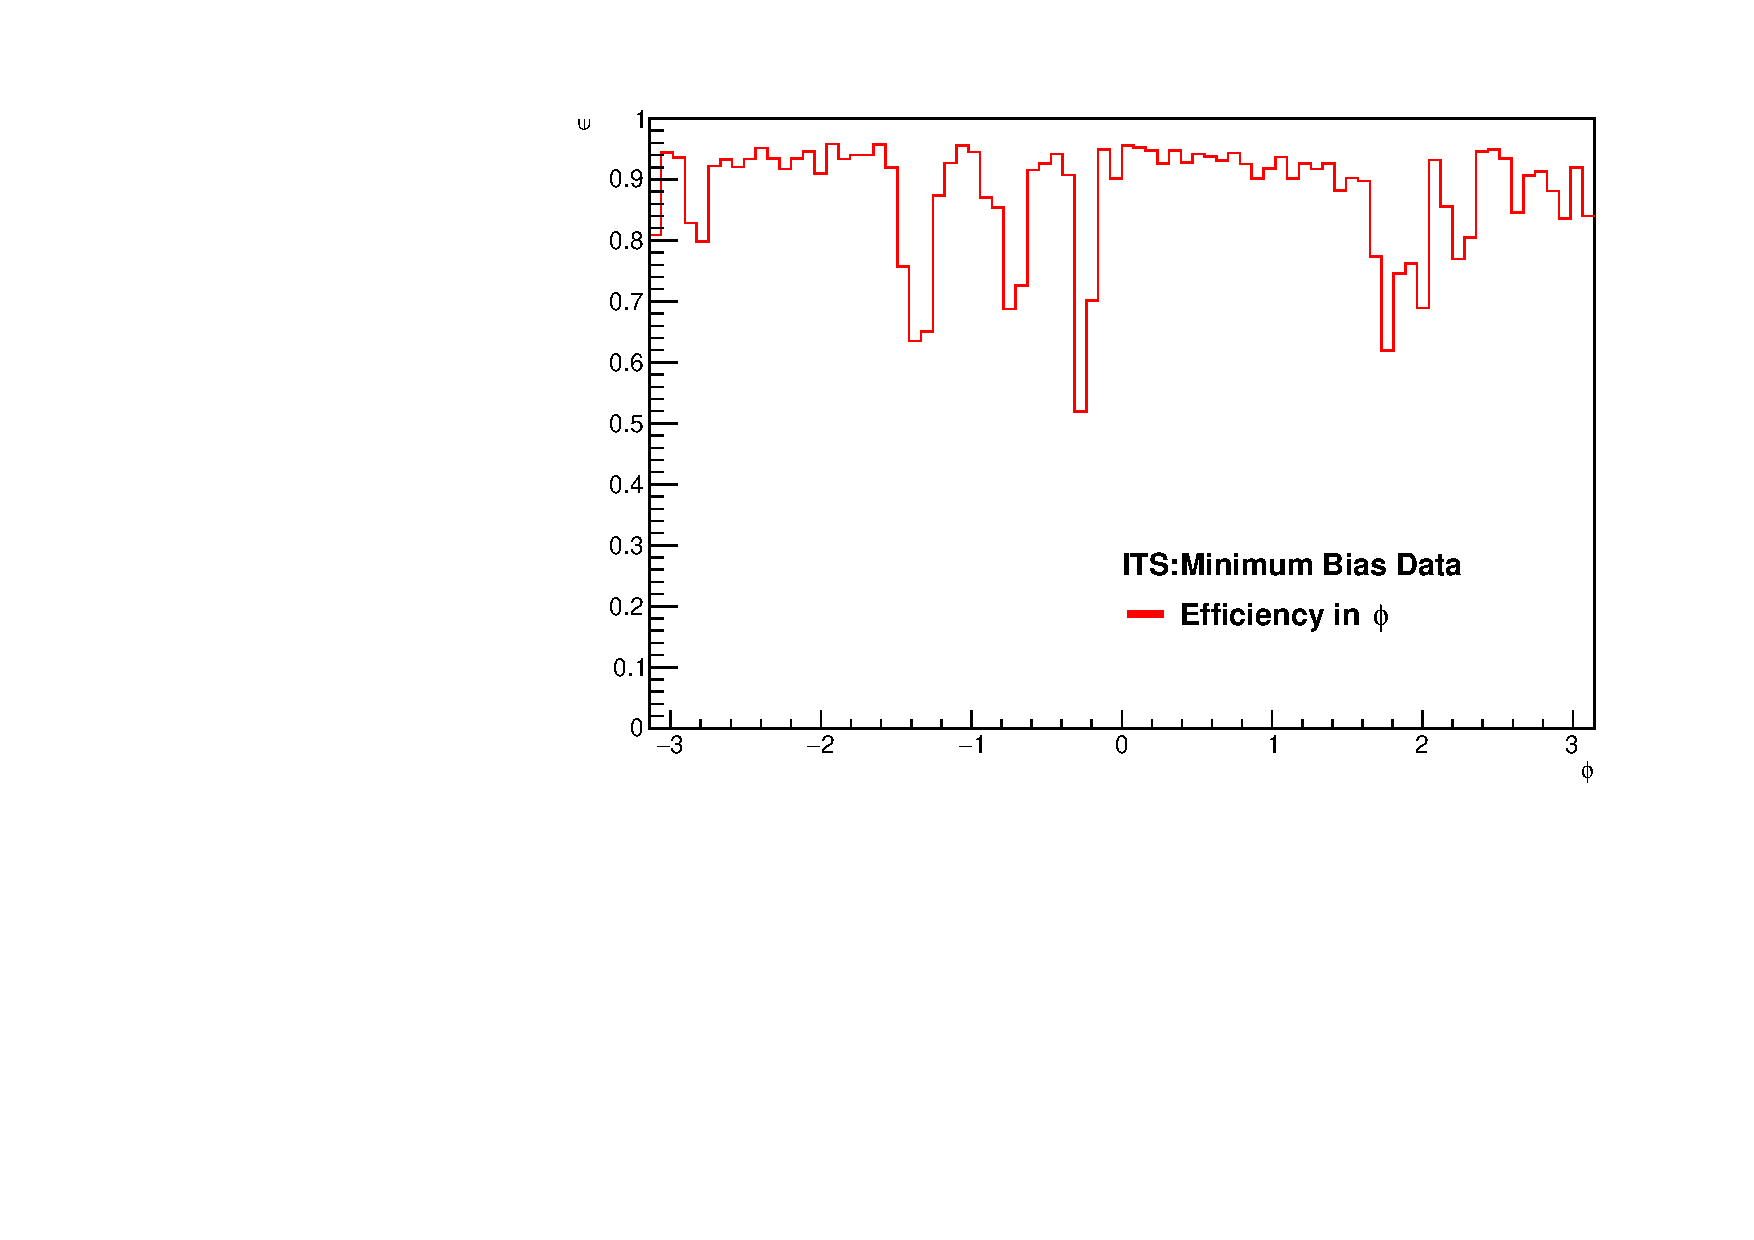
\includegraphics[width=.495\textwidth]{Data_Analysis/Tracking/its_phi_eff.pdf}
\caption{Tracking efficiency as a function of $\phi^{\mathrm{true}}$ for TPC+ITS tracks (left) and ITS-only tracks (right). In both cases, the efficiency is calculated for tracks with $\pt^{\mathrm{true}}>$ 1 \GeVc~using the LHC13b2\_efix\_p1 Monte Carlo simulation.}
\label{fig:phiEff}
\end{figure}

\begin{figure}[htpb]
\center
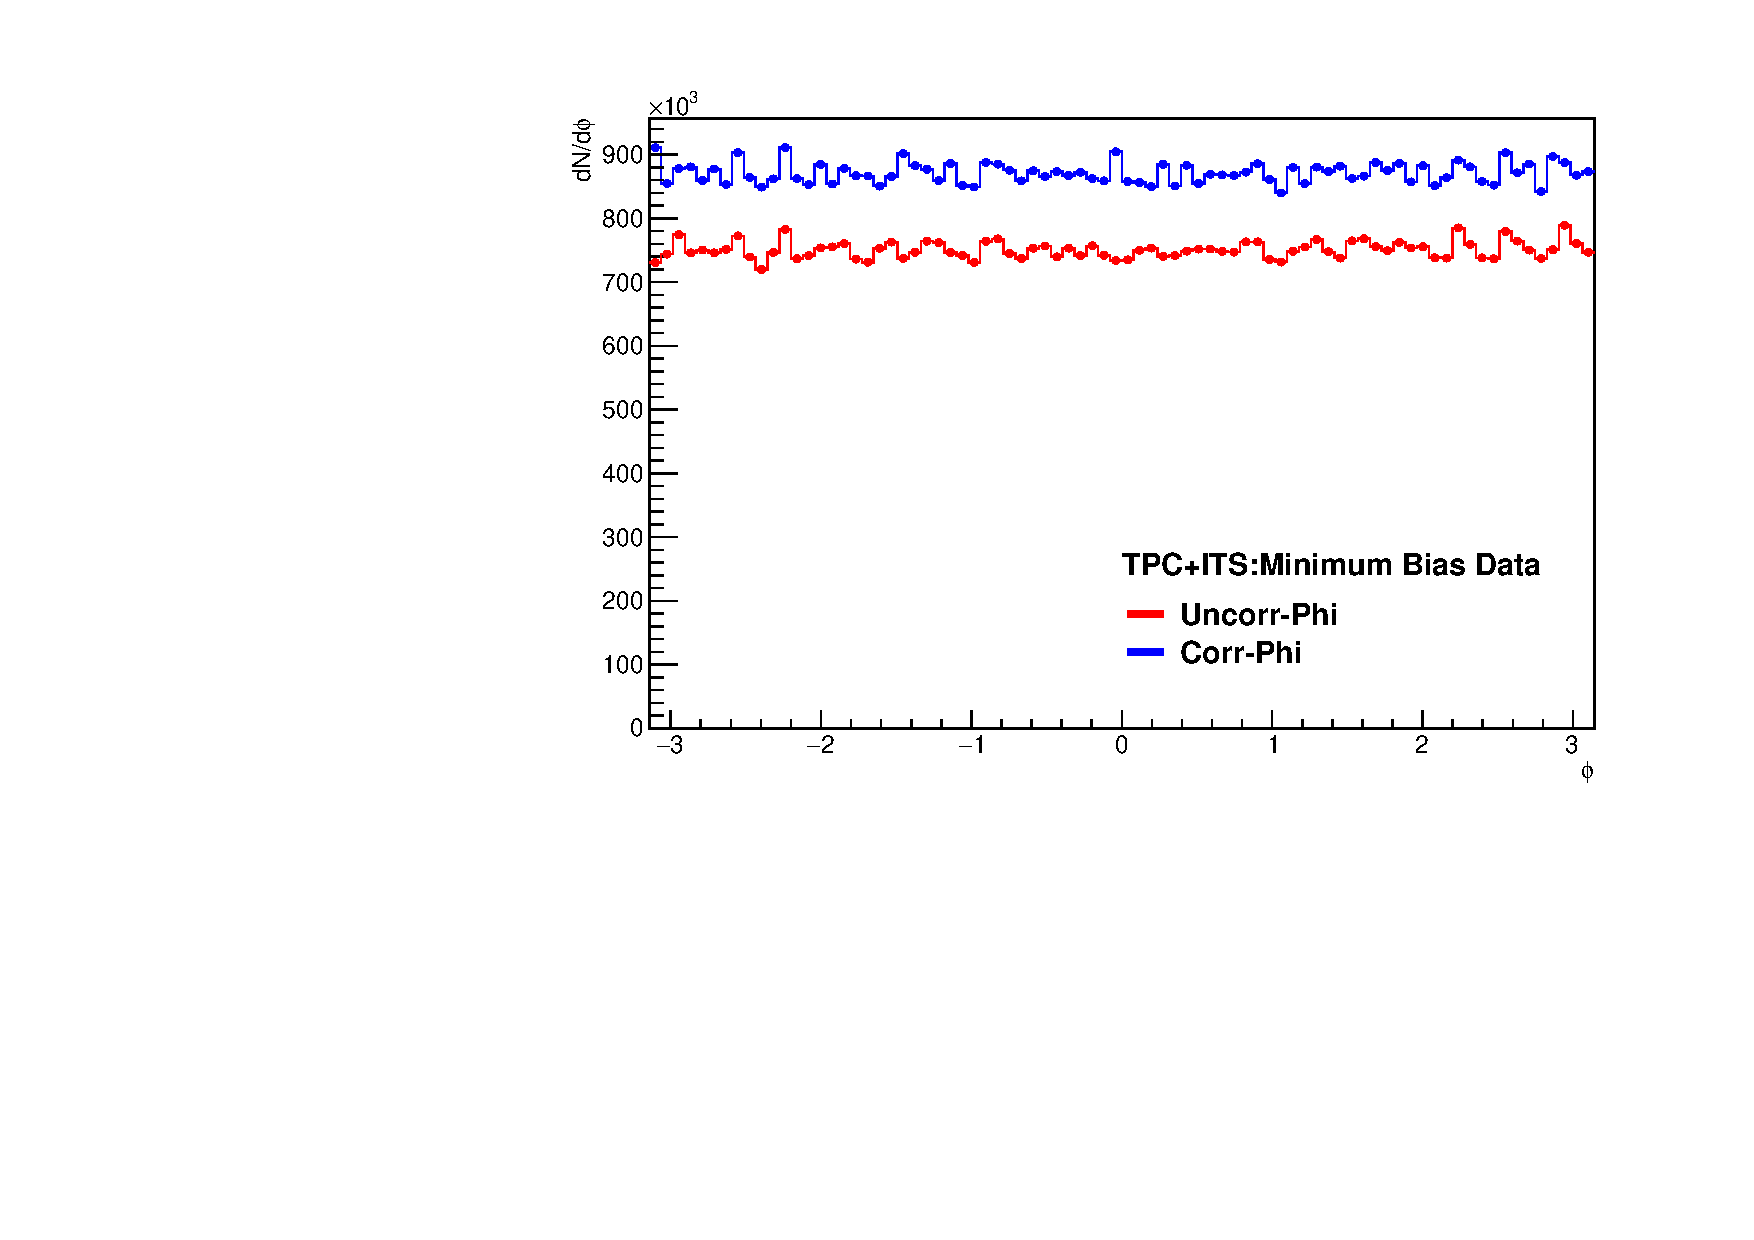
\includegraphics[width=.495\textwidth]{Data_Analysis/Tracking/phi_efficiency_cor_tpc.pdf}
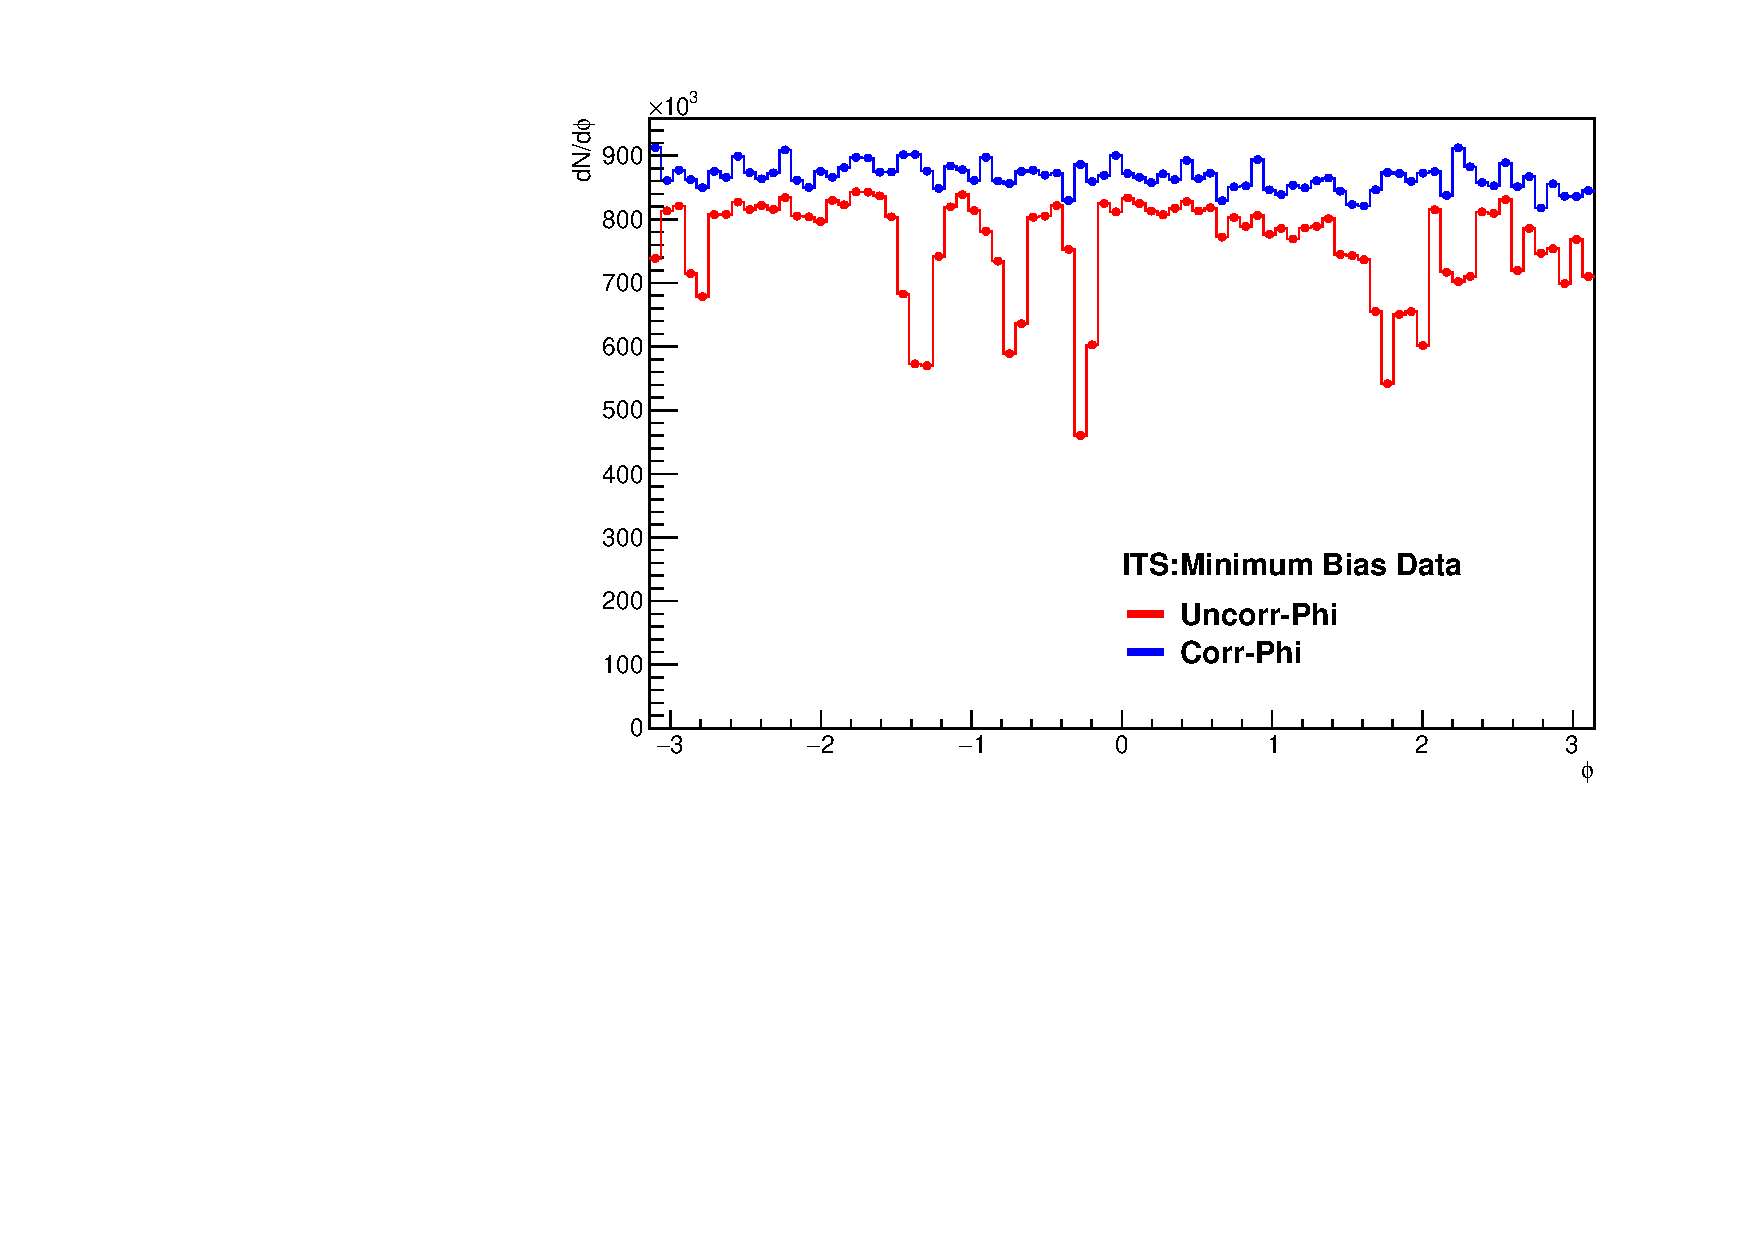
\includegraphics[width=.495\textwidth]{Data_Analysis/Tracking/phi_efficiency_cor_its.pdf}
\caption{Left panel: track $\varphi$ distribution measured in data for tracks with $|\eta|<0.8$ before (red) and after (blue) applying the efficiency correction for TPC+ITS tracks. Right panel:track $\varphi$ distribution measured in data for tracks with $|\eta|<0.8$ before (red) and after (blue) applying the efficiency correction for ITS-only tracks.}
\label{fig:phiCorr}
\end{figure}

Figure~\ref{fig:phiCorr} shows the $\varphi$ distribution of TPC+ITS and ITS-only tracks in minimum-bias \pPb~data and the effect of applying the efficiency correction to the $\varphi$ distribution. Before applying the efficiency correction, there are visible holes at $\varphi$ = $-$1.04, $-$0.8, $-$0.2 rad in ITS-only tracks which are not present in the TPC+ITS tracking. After applying the $\varphi$ efficiency, the holes are corrected, and a distribution which is flat within {$\pm$2.5\%} is obtained. The TPC+ITS remains flat after the efficiency correction, as expected. This shows that the description of dead channels in the ITS is well-described in the simulation. 


\subsection{Hybrid tracking on isolation check}

\subsection{Summary of the ITS-only Tracking Performance Studies} 
This section summarizes the findings of the studies on ITS-only tracking performance: 
\begin{enumerate}
\item Tracking Efficiency: \\
The ITS-only tracking efficiency is $75\%$ at 150 MeV/$c$ and grows to 85$\%$ at 1 \GeVc~and above. 
\item Fake rate:\\
The fake rate of ITS-only tracking is about 10 times worse than for TPC+ITS tracks, but still less than 20$\%$ below 10 \GeVc, which is the relevant range for the analyses presented in this note.
\item Momentum resolution:\\
The momentum smearing effects are significant for ITS-only tracking. The bin-to-bin correction factor due to smearing effects for ITS-only tracking is 0.7 at 10~\GeVc~and 0.5 at 15~\GeVc. The smearing effects for ITS+TPC tracking are negligible.
\item Description of $\varphi$ holes\\
The efficiency as a function of $\varphi$ shows inhomogeneity not present in the TPC+ITS tracking that are attributed to dead staves in the ITS. These are concentrated in specific $\eta$ and $\varphi$ regions. These are well described in the simulation. 
\end{enumerate}

These studies validate the MC corrections for tracking efficiency, fake rate and momentum smearing by comparing with published data. From that study, the combined systematic uncertainty on tracking performance is estimated to be a relative $\pm 5\%$ for ITS-only tracks with $0.5 < \pt < 10$ \GeVc. 

\FloatBarrier
\section{Neutral Energy in Isolation Variable}

In this analysis, the isolation variable was constructed using only charged-particles. In principle, neutral particles could have been added as well in the isolation definition. However, that would have limited the acceptance the measurement. For example, the recent ALICE isolated photon paper~\cite{Acharya:2019jkx} restricted the pseudorapidity of the $\gammaiso$ to $|\eta|<0.27$ to ensure a good containment of the isolation cone that has a radius of $R=0.4$ (the EMCal acceptance is $|\eta|<0.67$). An acceptance limitation would have a large impact of this analysis in terms of statistical precision, so a ''charged-only'' isolation isolation was chosen. This is not different than several ALICE jet analyses that report ''charged-only" jets and not ''full-jets''. 

\textsc{Pythia8} events are used to estimate the impact on the isolation variable of including neutral-particles. Figure~\ref{fig:PythiaNeutralIsolation} shows the comparison of the prompt-photon hadron correlations according to \textsc{Pythia8} when using no isolation requirement; with an isolation variable based on charged particles (used in this analysis); and with an isolation variable based on both charged-particles and neutral particles. In all cases, the charged-particles and neutral particles are final-state particles and have $\pt>150$ MeV/$c$ and $|\eta|<0.8$. No significant difference between the selection of 1.5 \GeVc~based on charged particles and the selection based on 2.0 \GeVc~based on charged and neutral particles was observed. Therefore, the $\iso<1.5$ \GeVc~selection is enough to suppress the near-side peak in the correlation functions coming from fragmentation photons, and that using neutral-particles in the isolation variable would not yield any significant improvement.

\begin{sidewaysfigure}[htpb]
\centering
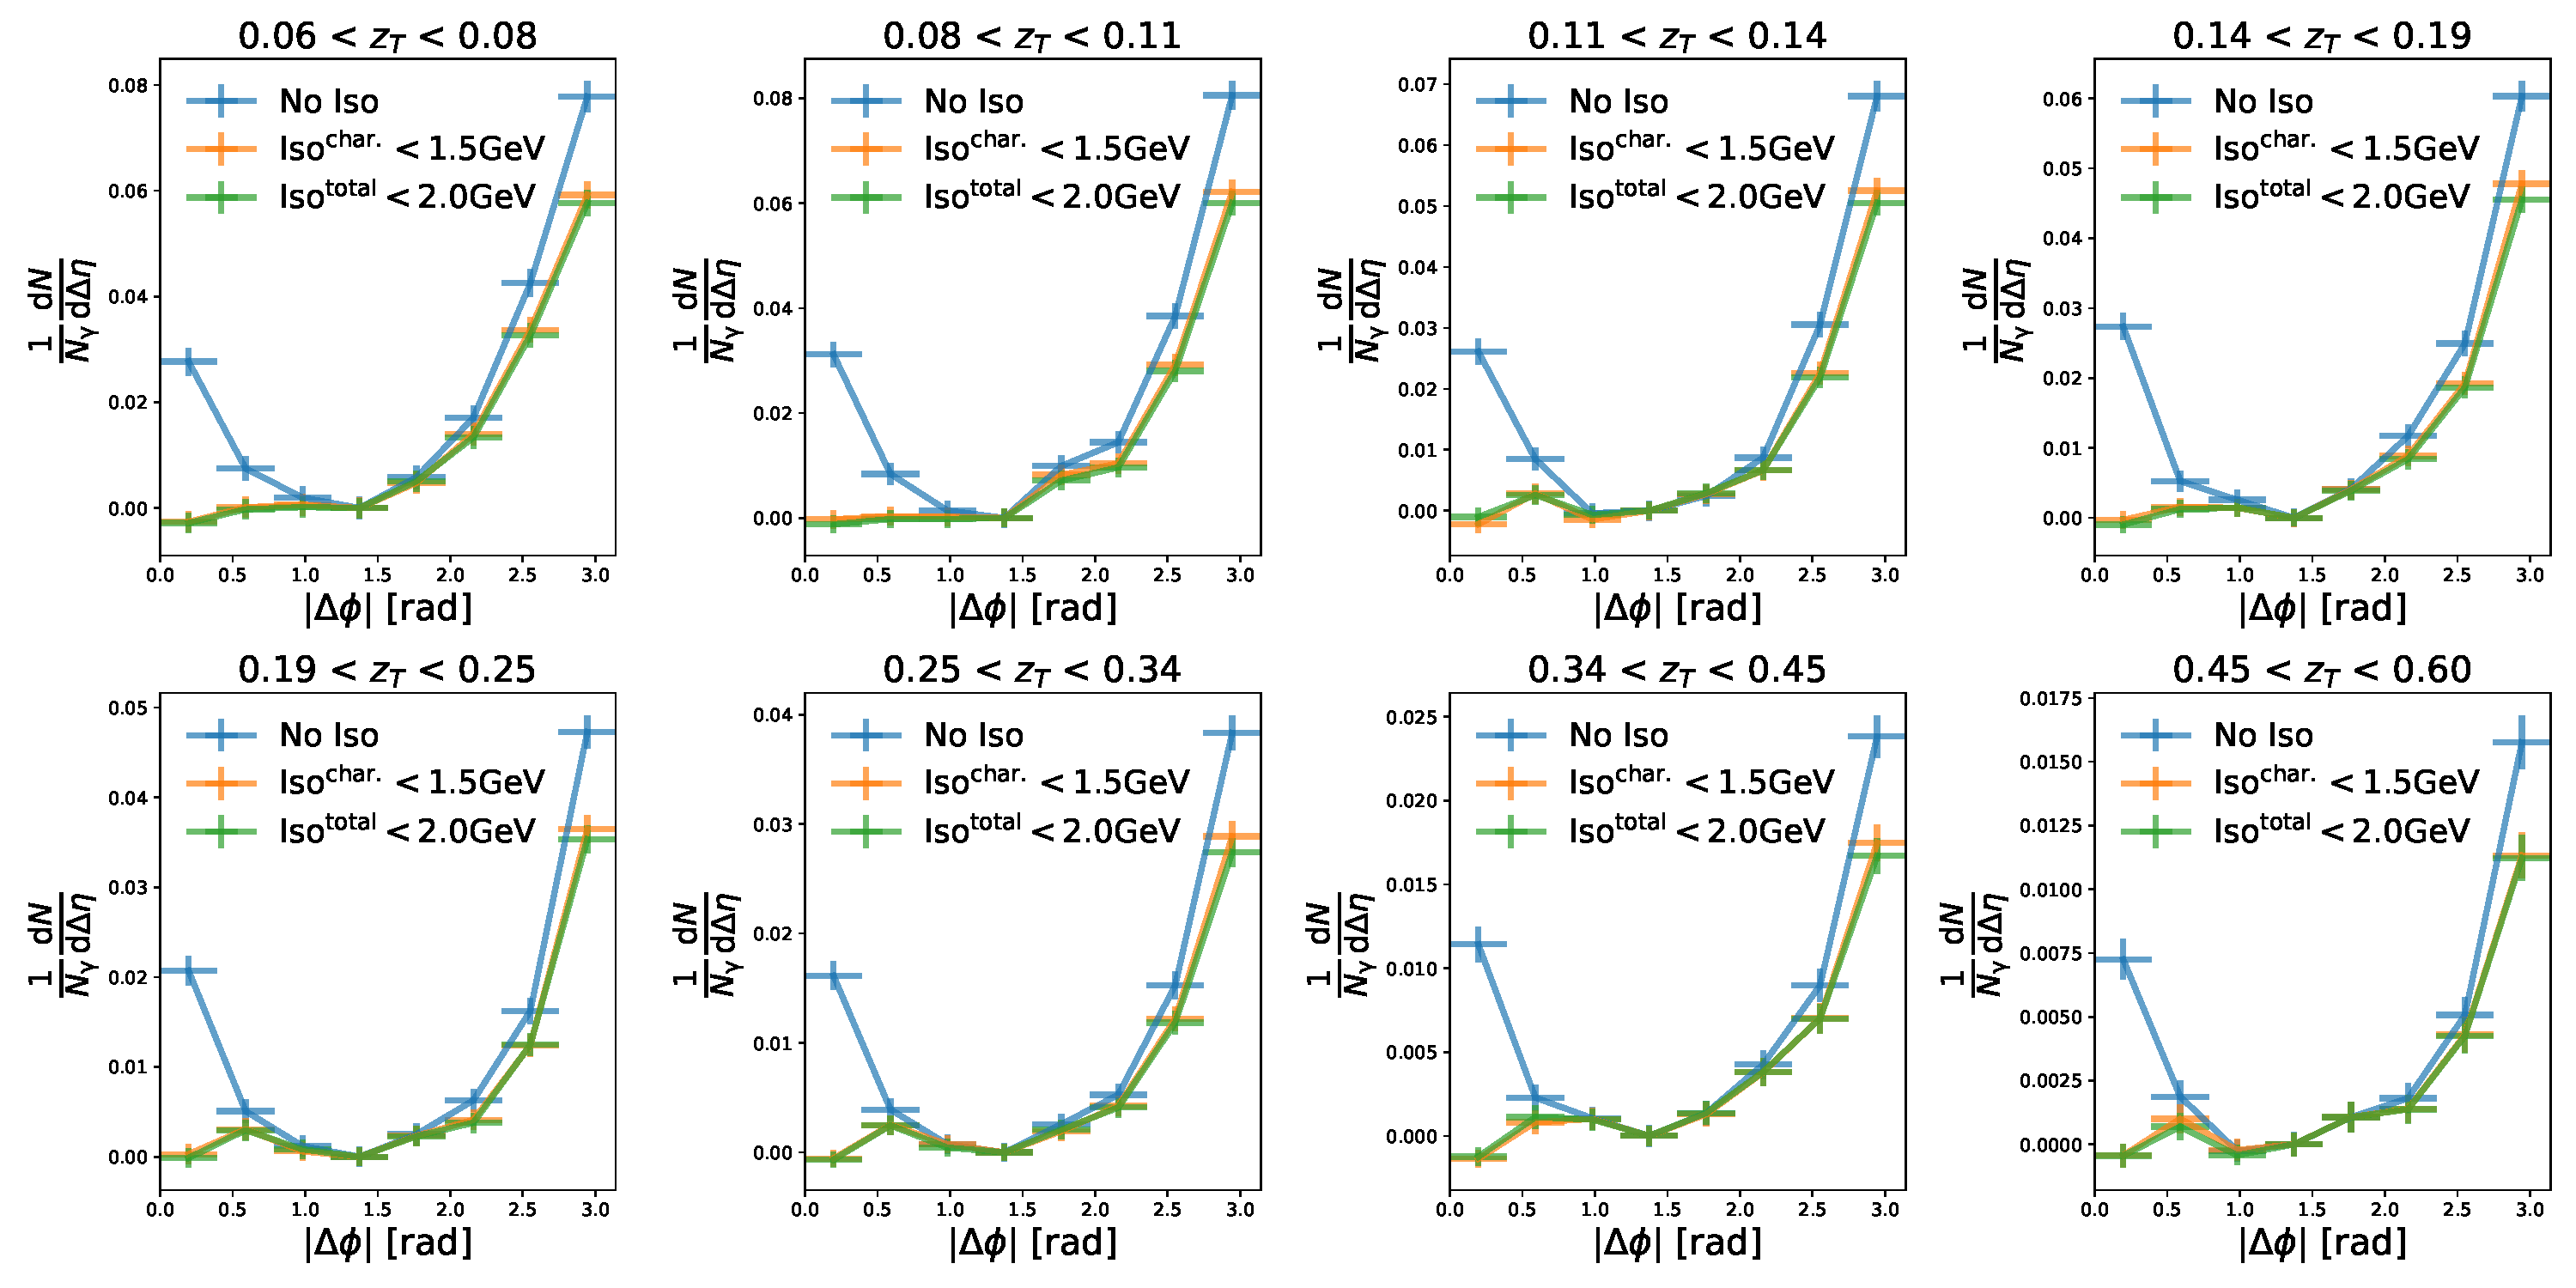
\includegraphics[width = 1.0 \textwidth]{Checks_Systematics/PythiaStudyNeutralIso}
\caption{Correlation function between prompt photons and hadrons from \textsc{Pythia8} for various \zt~bins. Three selections on the prompt photons based on isolation are presented: no isolation (blue); $\iso< 1.5$\GeVc~that considers only charged-particles (orange); and $\iso<2.0$ \GeVc~that considers both charged and neutral particles (green). In all cases, the uncorrelated background has been subtracted using the ZYAM method. The error bar represent statistical uncertainty only. }
\label{fig:PythiaNeutralIsolation}
\end{sidewaysfigure}


\section{Impact of Acceptance Difference Between pp and \pPb~due to Boost}
\label{sec:bootstudy}

In this section, the impact of the acceptance difference between pp and \pPb~data that arises due to the boost in \pPb~data is estimated. The boost in \pPb~data arises due to the energy difference between the proton and lead beam, and it amounts to a rapidity difference of $\Delta y = 0.47$  in the proton-going direction. That means that in \pPb~collisions, the lab acceptance for photons that is $-0.67<\eta<0.67$ corresponds to $-0.2<\eta<1.14$ in the center-of-mass frame, whereas the charged-particle acceptance of $-0.8<\eta<0.8$ corresponds to $-0.33<\eta<1.27$  in the center-of-mass frame. 

\textsc{Pythia8} events are used to estimate what is the difference between \gammaiso--hadron correlations with the acceptance of $\gammaiso$ and charged particles  $-0.20<\eta<1.14$ and $-0.33<\eta<1.27$ instead of the nominal ranges of $-0.67<\eta<0.67$ and $-0.8<\eta<0.8$. This is shown in Figure~\ref{fig:PythiaBoostStudy}. The boosted acceptance results in about a 5\% lower $\gammaiso$--hadron correlation compared to the nominal acceptance, irrespective of \zt~range. For illustration purposes, the impact of a boost of $\Delta y =1.0$ is plotted, which shows a decrease of about 15$\%$  with respect to the nominal acceptance, irrespective of \zt~range. 

\begin{sidewaysfigure}[htpb]
\centering
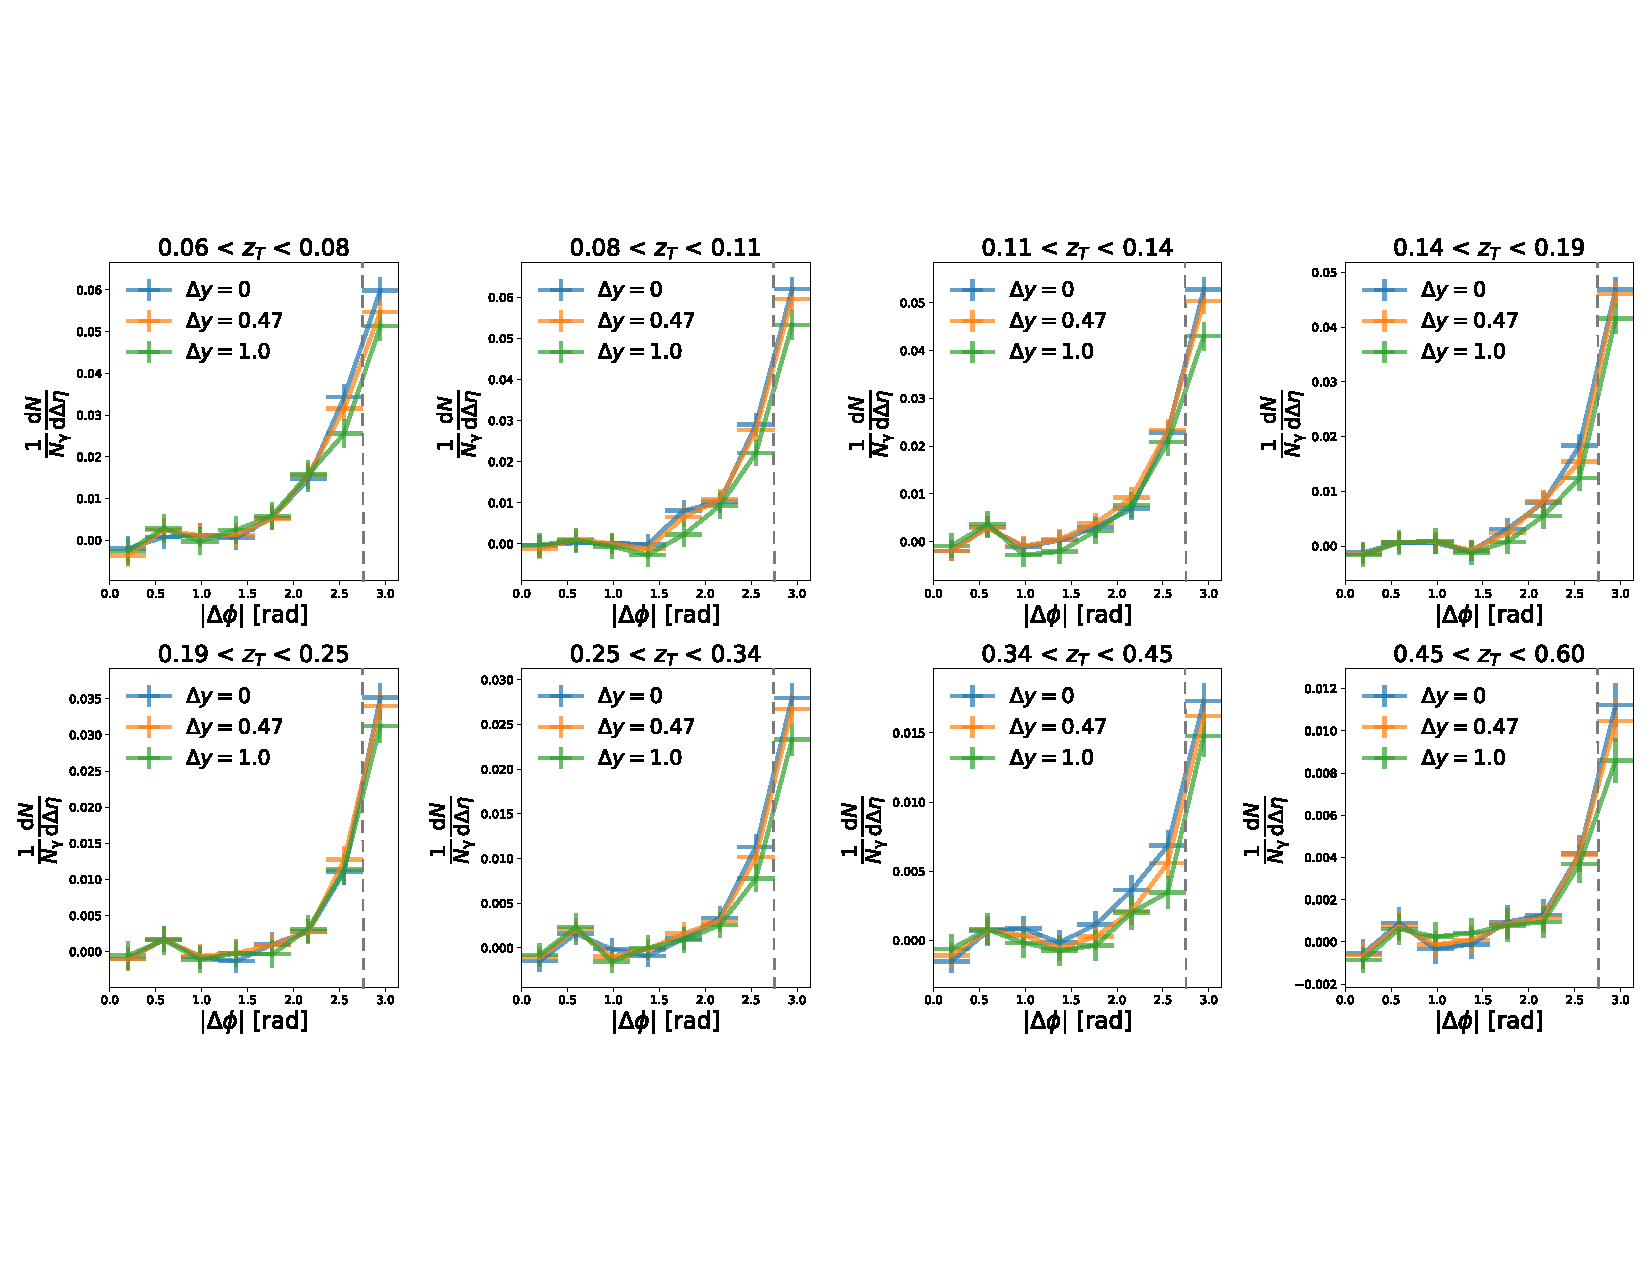
\includegraphics[width = 1.0 \textwidth]{Checks_Systematics/PythiaStudyBoost_wLines}
\caption{Correlation function between isolated prompt photons and hadrons from \textsc{Pythia8} for various \zt~bins. The nominal result ($\Delta y =0$, in blue) is compared with results obtained with a kinematic selection that mimics the boost of \pPb~data (orange). For illustration purposes, the impact of a boost that is larger than the one of \pPb~data ($\Delta y = 1.0$ in green) is shown. The dashed lines at $\varphi = \frac{7\pi}{8} $ indicates the integration window used to obtain the away side yields.}
\label{fig:PythiaBoostStudy}
\end{sidewaysfigure}

The chosen integration window (dashed lines) in the figure above makes it clear what effect this may have on the final away side yields. Thus the effect of acceptance the mismatch in this analysis is limited due to the relatively small boost of $\Delta y = 0.47$ and the limited acceptance of EMCal and ITS, which even with boost is within mid-rapidity region where the cross-sections do not change drastically. 

\label{sec:EfficiencyAppendix}
% \addtocontents{toc}{\protect\setcounter{tocdepth}{0}}
\section{Isolated-photon Efficiency}

Because the correlation functions are normalized per photon trigger, the photon efficiency cancels. In principle, a bias may be introduced if the photon efficiency varied rapidly within the photon \pt~range being used (12--40 \GeVc) but this section will show that this is negligible.  

The efficiency the isolated-photon selection is shown in Figure~\ref{fig:photonEff_pPb}. The efficiency is rather independent of \pt~in the range relevant for this analysis. Less than 1\% variation is observed between the high and low ranges of the energy distribution of the photon triggers (77.7\% at 12 \GeVc~and 78.5\% at 40 \GeVc). This level of variation has a negligible impact in the correlation analysis. 
\begin{figure}
\centering
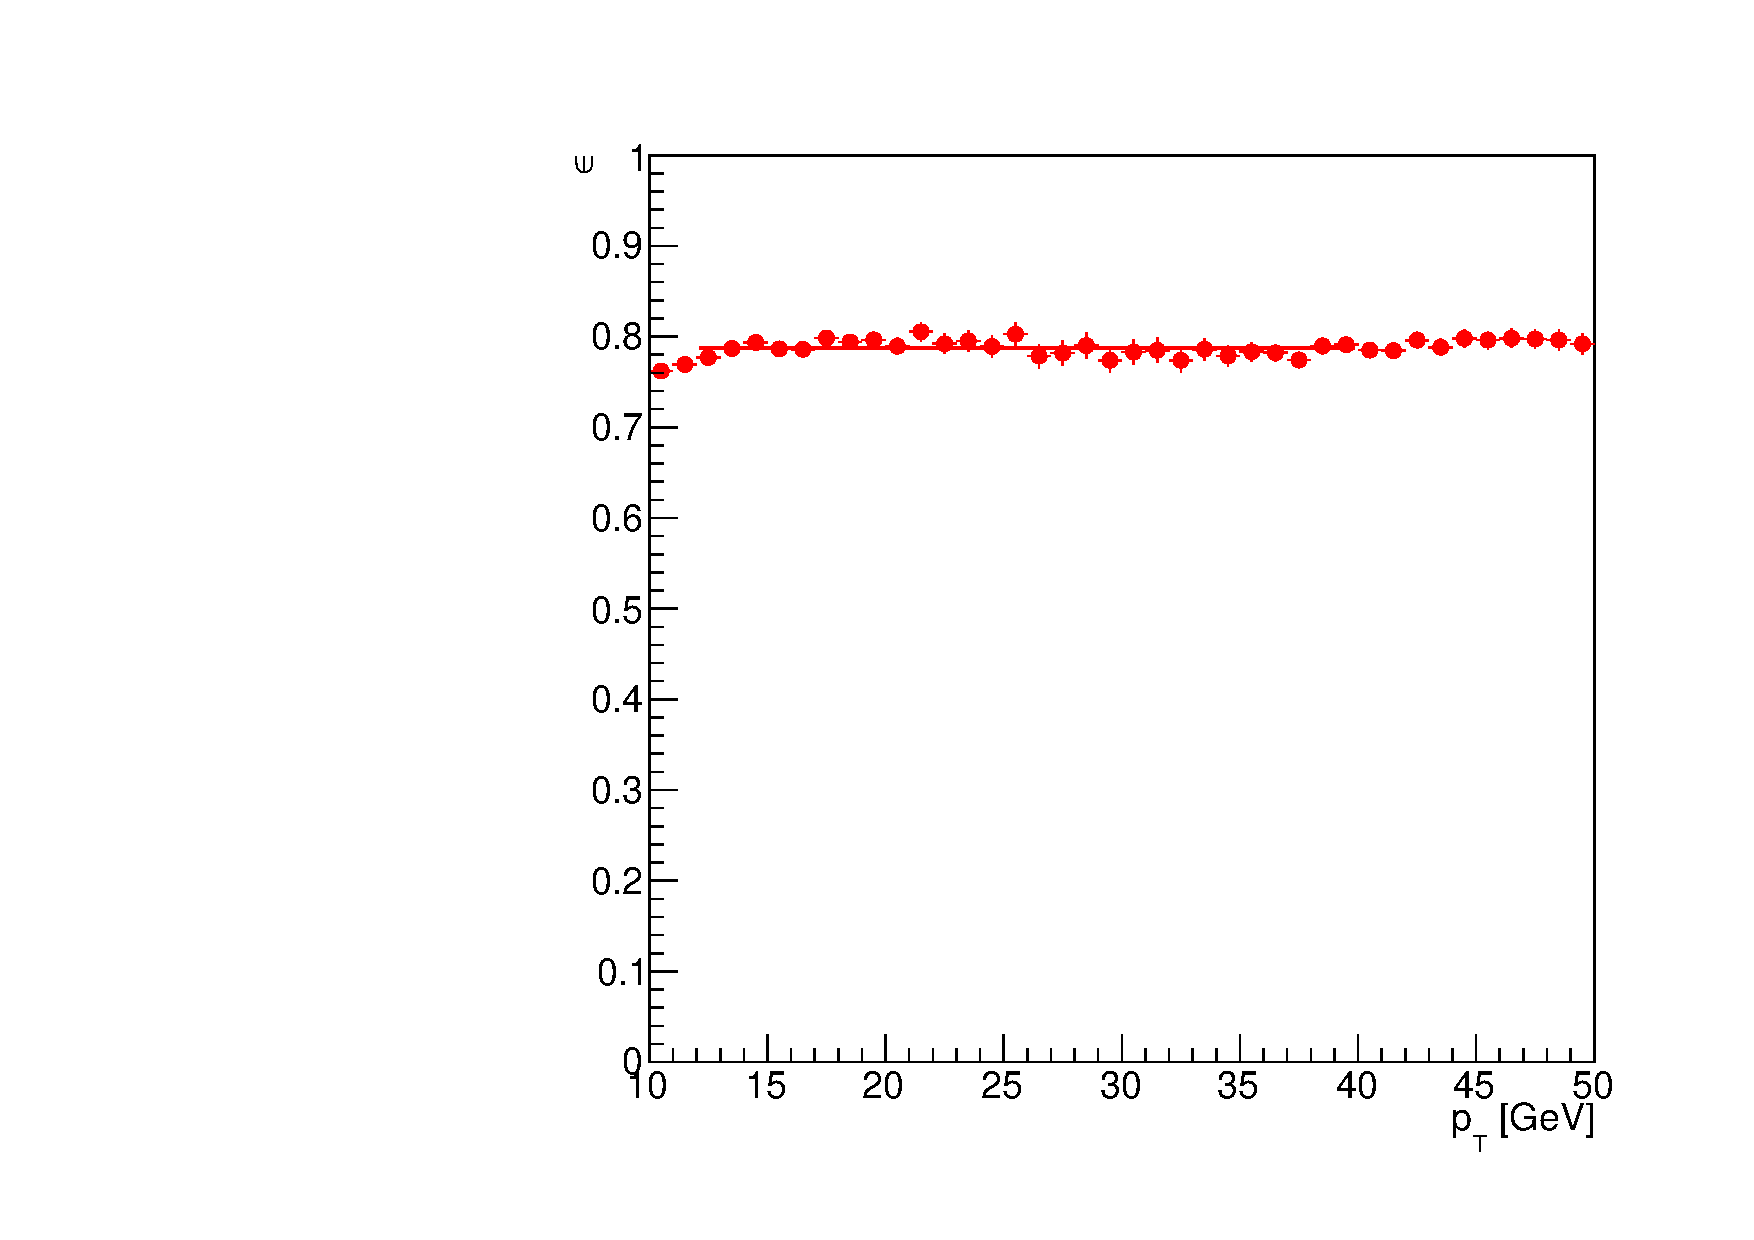
\includegraphics[width=0.45\textwidth]{Checks_Systematics/Efficiency_photon_pPb}
\caption{Isolated-photon efficiency obtained with \pPb~simulation.}
\label{fig:photonEff_pPb}
\end{figure}

%\FloatBarrier
\section{Comparison to ABCD method results}
\label{sec:comparisontoABCD}
In this section, the results obtained with the template fit method are compared to the ABCD method results obtained by Erwann Masson for his isolated-photon analysis in \pPb~data~\cite{Erwann}. That study is performed with the same \pPb~data using the same event and cluster selections and a similar isolation criterion that uses only charged-particles (shown in the Appendix of Ref.~\cite{Erwann}).

Figure~\ref{fig:ComparisonToErwanns} shows the results compared to the results of the ABCD method. Both the results using ITS-only tracks and ITS-TPC tracks (which is more directly comparable to the ABCD result) are shown. The results are systematically below the ABCD method, but they are consistent within 1$\sigma$ systematic uncertainty for most of the $\pt$ range. 
%Given that the two methods are independent, and the systematic uncertainties are estimated independently, this level of agreement in principle constrains the systematic uncertainties, although a full evaluation of the correlation of the systematic uncertainties of the two methods is outside the scope of this analysis. 

%Previous analyses of isolated photons have used the ``matrix'' or ``ABCD'' method with an isolation variable that considers both charged particles and calorimeter clusters. The issue of bias due to the ``factorization'' assumption, i.e the correlation between the isolation variable and the shower-shape variable, has been studied in great detail\footnote{See for example D. Lodato's thesis, CERN-THESIS-2017-307.}. It has been shown that the ``non-factorization" bias comes from neutral energy in the isolation because that introduces a correlation through meson decays. The use of an isolation variable that only considers charged-particles limits the biases, corrections and associated systematic uncertainties, at the expense of a slightly lower purity. 

\begin{figure}[h]
\center
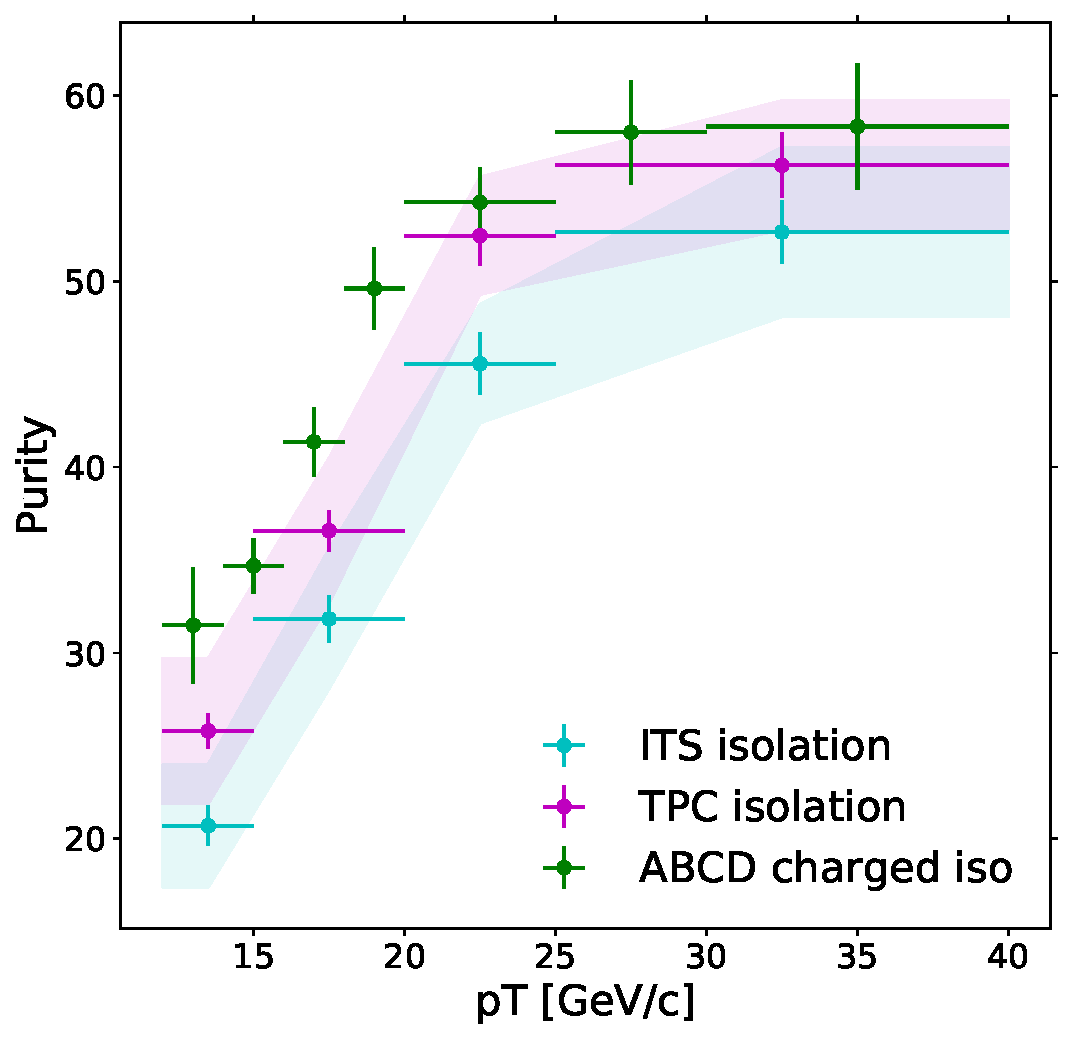
\includegraphics[width=0.5\textwidth]{Checks_Systematics/ABCDcomparison.pdf}
\caption{Comparison between purity measured with the template fit and ABCD method, from Ref.~\cite{Erwann}, in \pPb~data. The error bars represent statistical uncertainty only and the bands represent the systematic uncertainty only.}
\label{fig:ComparisonToErwanns}
\end{figure}



\section{Check by splitting clusters in $|\eta|<0.4$ and $0.4<|\eta|<0.67$ }

In this analysis, only clusters with $|\eta|<0.67$ (Section~\ref{sec:clusterselection}) are used, with an isolation variable constructed with tracks with $|\eta|<0.8$ (Section~\ref{sec:tracking}) and a cone size of $R=$0.4 (Section~\ref{sec:isolation}). The isolation cone is thus fully contained in the tracking acceptance only for clusters with $|\eta|<0.4$; the isolation cone for clusters with $0.4<|\eta|<0.67$ is only partially covered in pseudorapidity angle. Note that the tracking acceptance covers the full azimuthal angle so this is not an issue in azimuth. 

To check for possible biases that this partial containment of isolation cone in pseudorapidity all measured clusters were split into two categories: $|\eta|<0.4$ and $0.4<|\eta|<0.67$. In principle, if the bias introduced by the lack of total coverage of the isolation cone would lead to higher background in the $0.4<|\eta|<0.67$ region (background might appear less-isolated than in reality, and might pass the selection), it should thus lead to a lower purity. This study is performed in \pPb~data, which has better statistical precision than the pp data and would allow us to better constrain small biases. The comparison of purity measurements is shown in Figure~\ref{fig:spliteta}. Both sets of measurements are compatible within statistical uncertainties. Thus, the potential bias due to incomplete coverage of isolation cone is negligible and any systematic uncertainty to this source is not assigned to the measurement. This observation may be explained by noting that the azimuthal angle is fully covered, and that most of the energy in the isolation cone is within small angles of the neutral-mesons that dominate the background (the background is primarily high-z neutral mesons in jets). 

\begin{figure}
	\center
	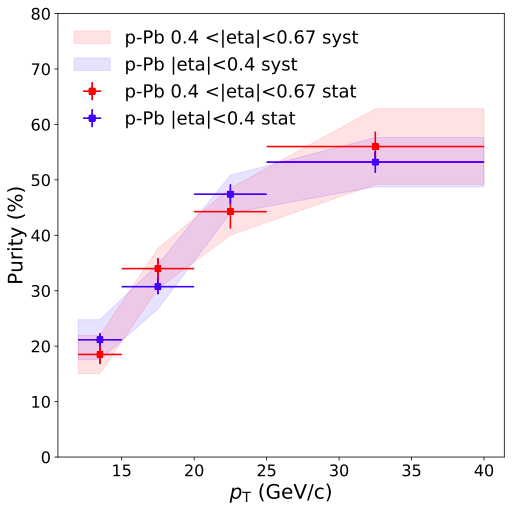
\includegraphics[width=0.5\textwidth]{Checks_Systematics/SplitEtaStudy}
	\caption{Purity measurement in \pPb~collisions for clusters with $|\eta|<0.4$ and $0.4<|\eta|<0.67$.}
	\label{fig:spliteta}
\end{figure}

\section{Cluster Selection Variations}
\label{sec:clustercutselectionvariation}
This section studies the impact of variations in the cluster selection (Section~\ref{sec:clusterselection}) on the purity measurement. It should be noted that the purity by itself is not a physical quantity. It is entirely cut-dependant, where a higher purity often results in a lower efficiency. As a result, the variations in this analysis are not used to estimate an uncertainty on the purity.

First, the impact of the number-of-local maximum criteria for clusters is studied. The NLM $<3$ selection was used in previous isolated photon analyzes (e.g. Ref~\cite{Acharya:2019jkx,Erwann}), where it was found to help to improve the simulation description of the background shower-shape. Figure~\ref{fig:numberoflocalmaxima} shows the purity measurement with and without this selection in pp and \pPb~data. No significant difference is observed.

\begin{figure}
	\center
	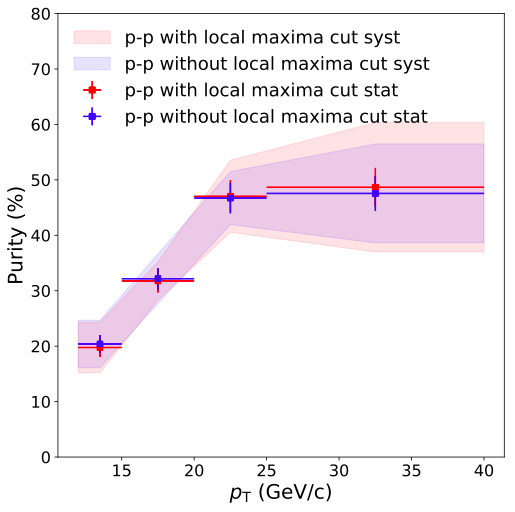
\includegraphics[width=0.495\textwidth]{G-H_New/dPhi_to_0/NLMvariation_pp.png}
	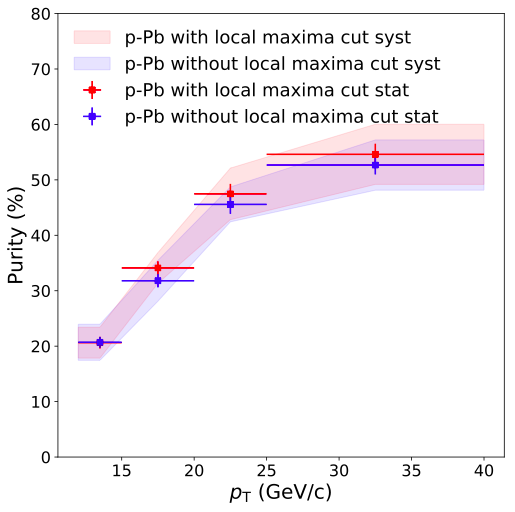
\includegraphics[width=0.495\textwidth]{Checks_Systematics/NLMvariation_pPb}
	\caption{Purity measurement with and without cluster selection based on number-of-local maxima in pp (left) and \pPb~(right) collisions.}
	\label{fig:numberoflocalmaxima}
\end{figure}

Figure~\ref{fig:distancetobadchannel} shows the purity measurement by varying the distance-to-bad channel cut from the nominal $\geq 1$ to $\geq 2$. This change would remove about 20$\%$ of the \gammaiso~candidates. Onec again, no significant difference is observed. 

\begin{figure}
	\center
	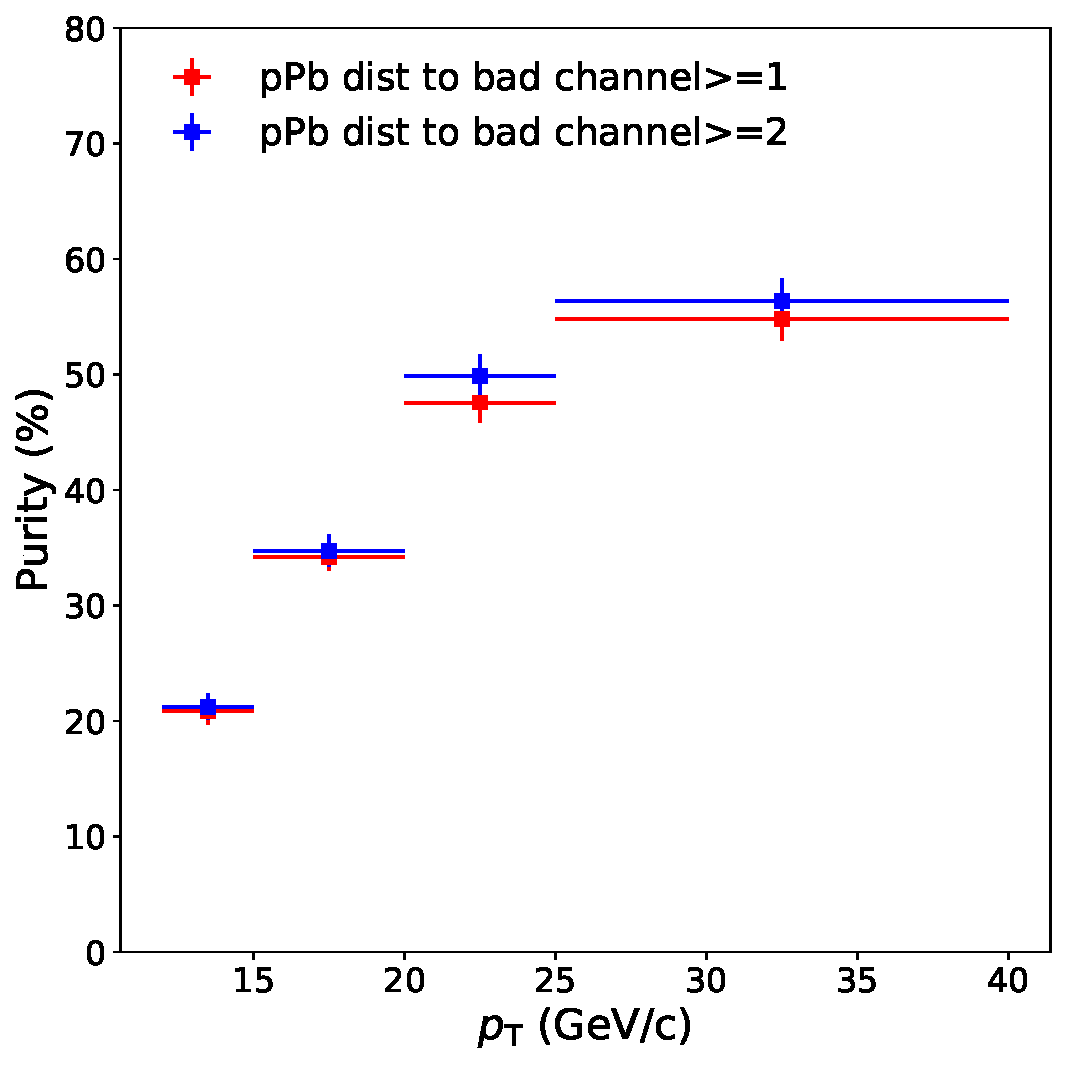
\includegraphics[width=0.495\textwidth]{Checks_Systematics/ppbdistance.pdf}
	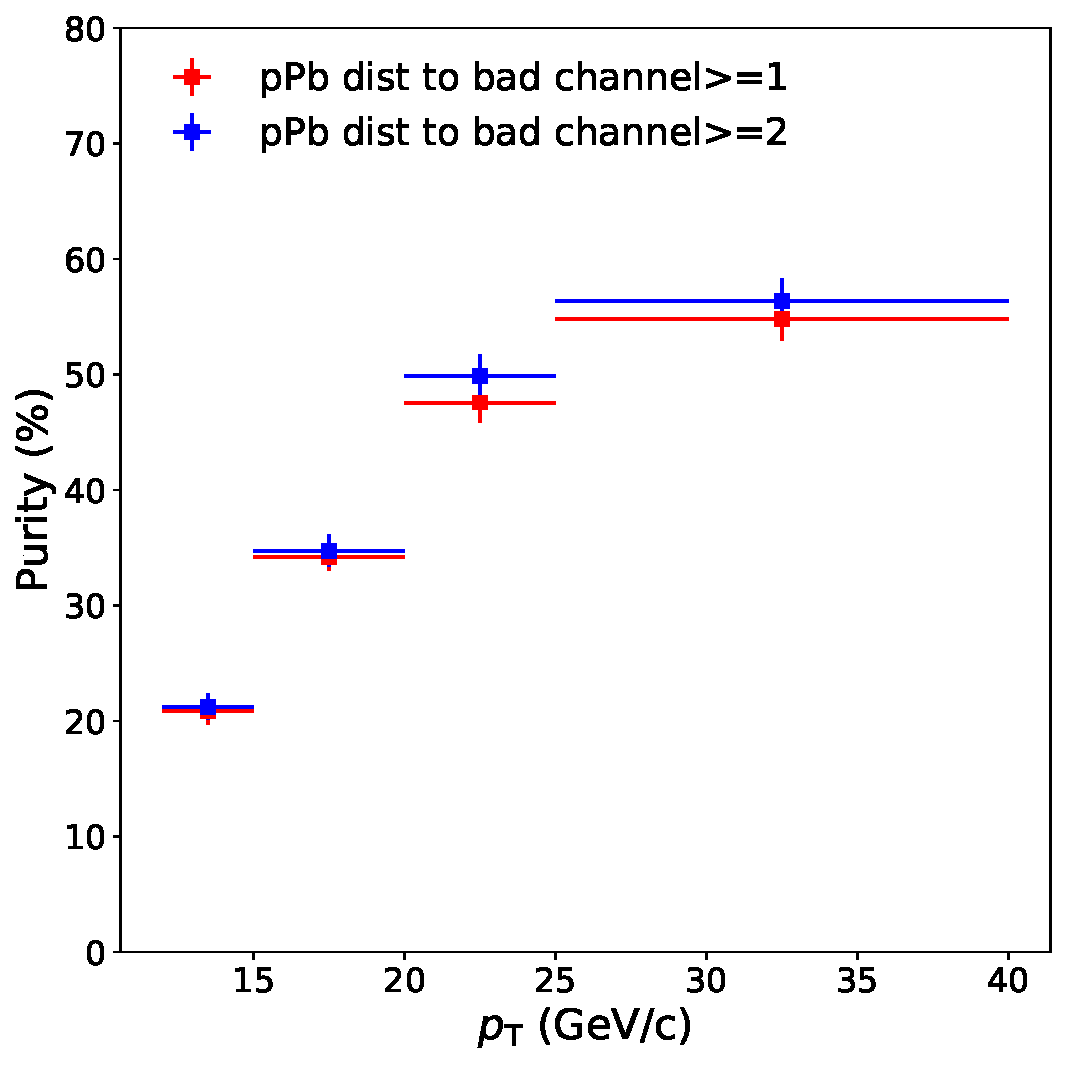
\includegraphics[width=0.495\textwidth]{Checks_Systematics/ppbdistance.pdf}
	\caption{Purity measurement with distance-to-bad channel $\geq 1$ (nominal) and $\geq 2$ in pp (left) and \pPb~(right) data.}
	\label{fig:distancetobadchannel}
\end{figure}

Figure~\ref{fig:TOF_purity} shows the purity measurement with and without cluster time selection. No significant difference is observed. 

\begin{figure}
	\center
	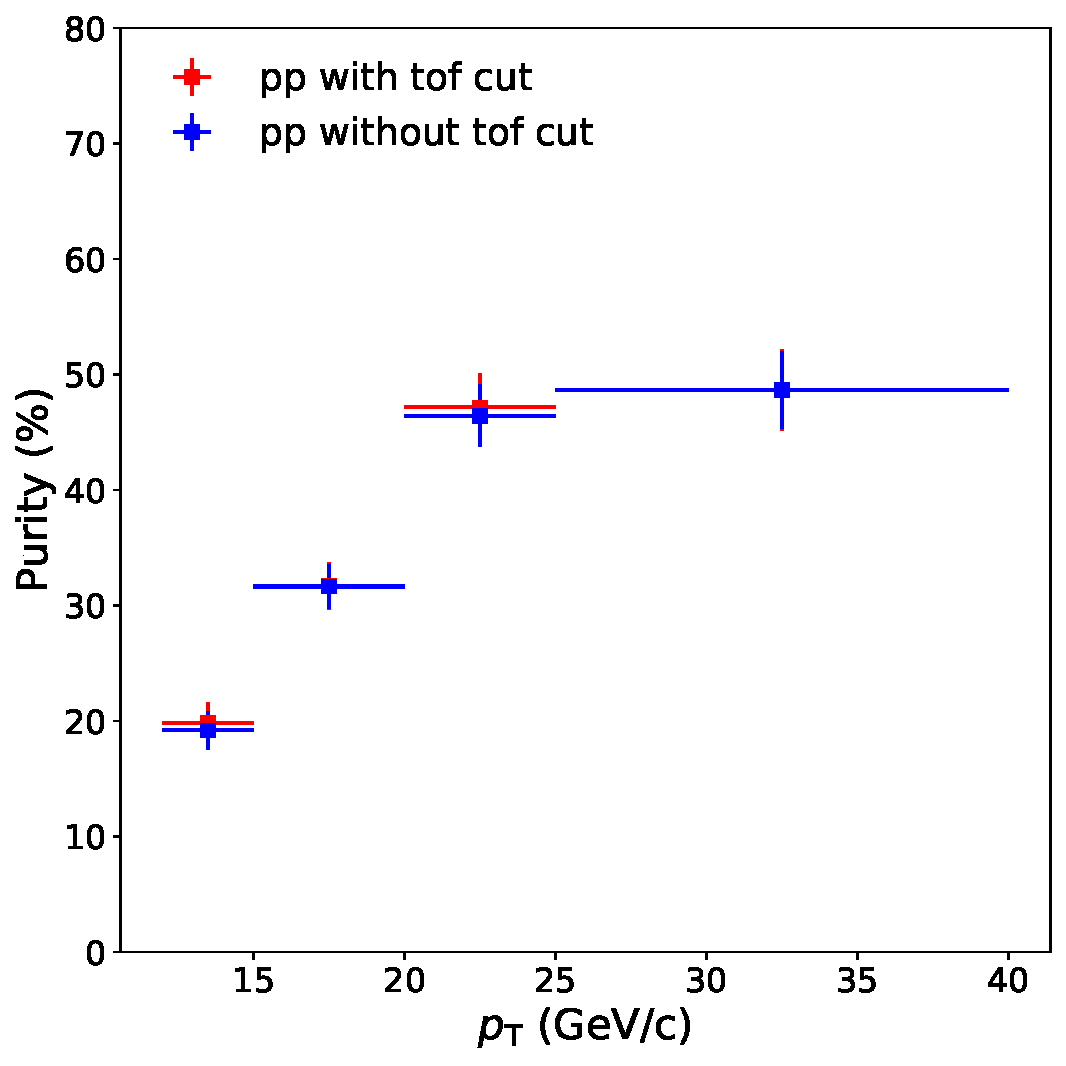
\includegraphics[width=0.495\textwidth]{Checks_Systematics/pptof.pdf}
	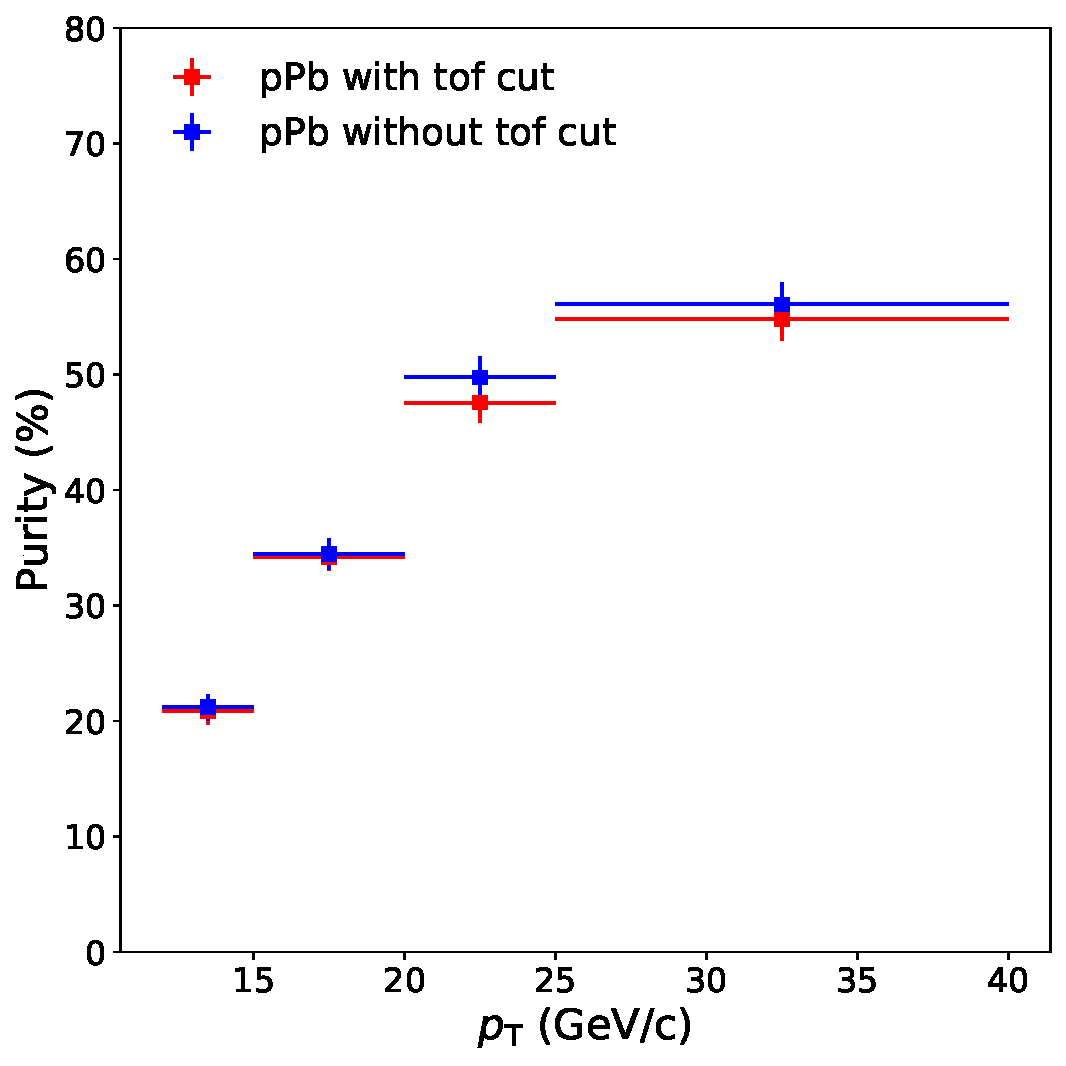
\includegraphics[width=0.495\textwidth]{Checks_Systematics/ppbtof.pdf}
	\caption{Purity measurement with and without time cut $(\Delta t<20$ ns) in pp (left) and \pPb~(right) data.}
	\label{fig:TOF_purity}
\end{figure}

Figure~\ref{fig:exoticity} shows the purity measurement with an exoticity cut with a threshold of 5\% (nominal) and a variation of $3\%$, with no significant difference shown. 

\begin{figure}
	\center
	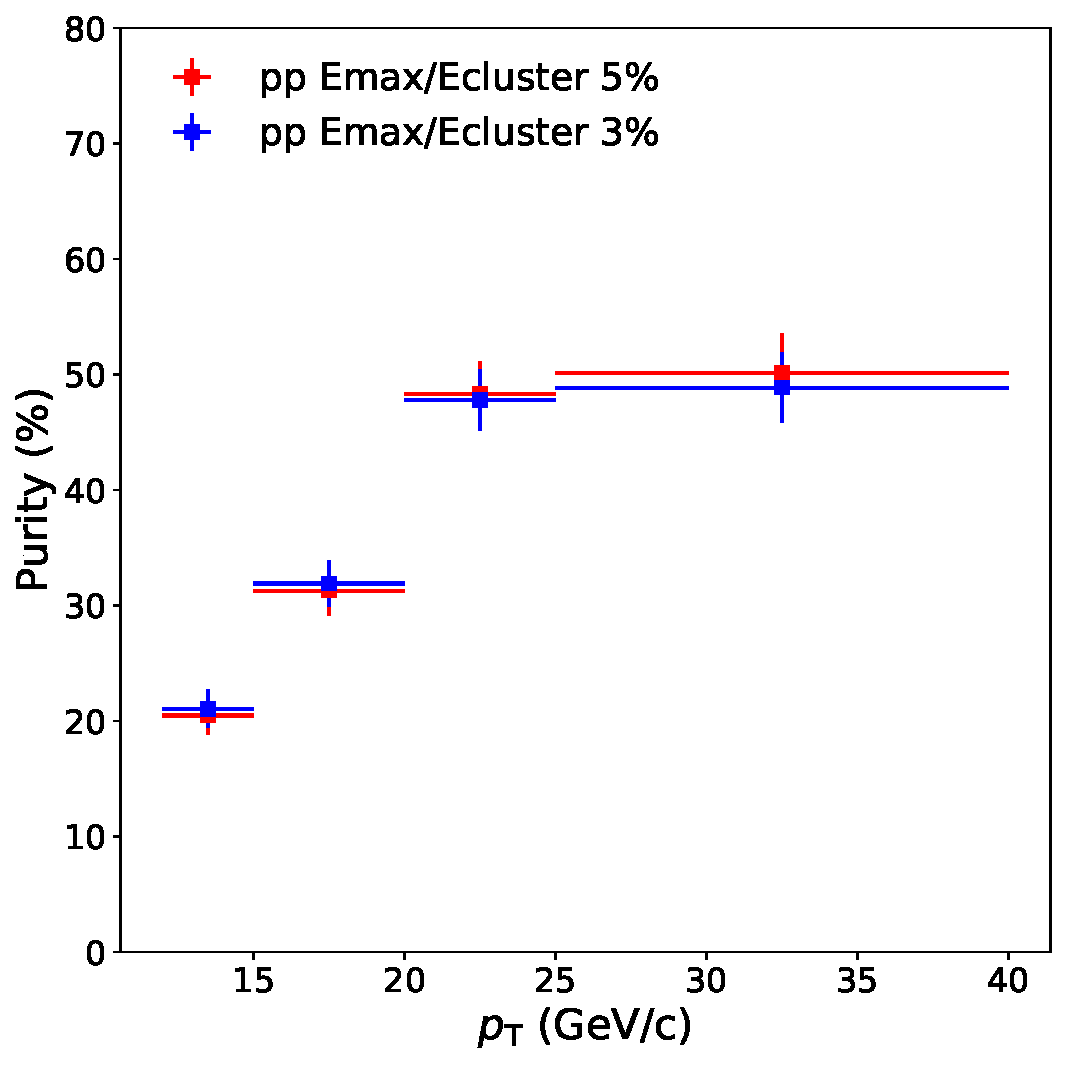
\includegraphics[width=0.495\textwidth]{Checks_Systematics/ppemax.pdf}
	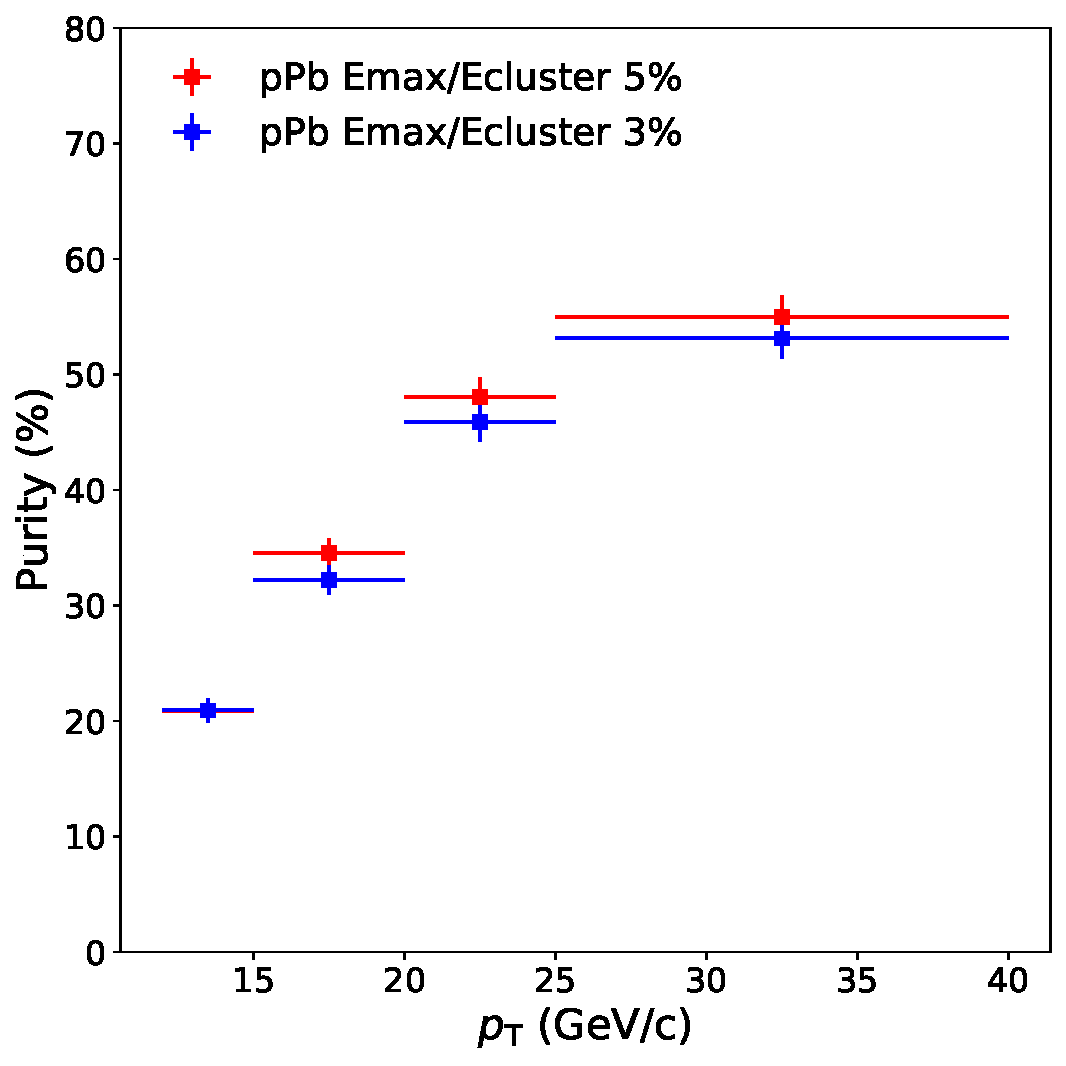
\includegraphics[width=0.495\textwidth]{Checks_Systematics/ppbemax.pdf}
	\caption{Purity measurement with an exoticity cut of 5$\%$ (nominal) and 3$\%$ in pp (left) and \pPb~(right) data.}
	\label{fig:exoticity}
\end{figure}

Figure~\ref{fig:isolationvariation} shows the purity measurement with different isolation thresholds. The nominal threshold of 1.5 $\GeVc$ is varied by $\pm$ 0.2 \GeVc. As expected the higher (lower) isolation threshold results in a lower (higher) purity. However, the difference with respect to the nominal result is small with respect to the statistical and systematic uncertainties. This indicates that the purity measurement has only a weak dependence on the choice of isolation threshold. 



\begin{figure}
	\center
	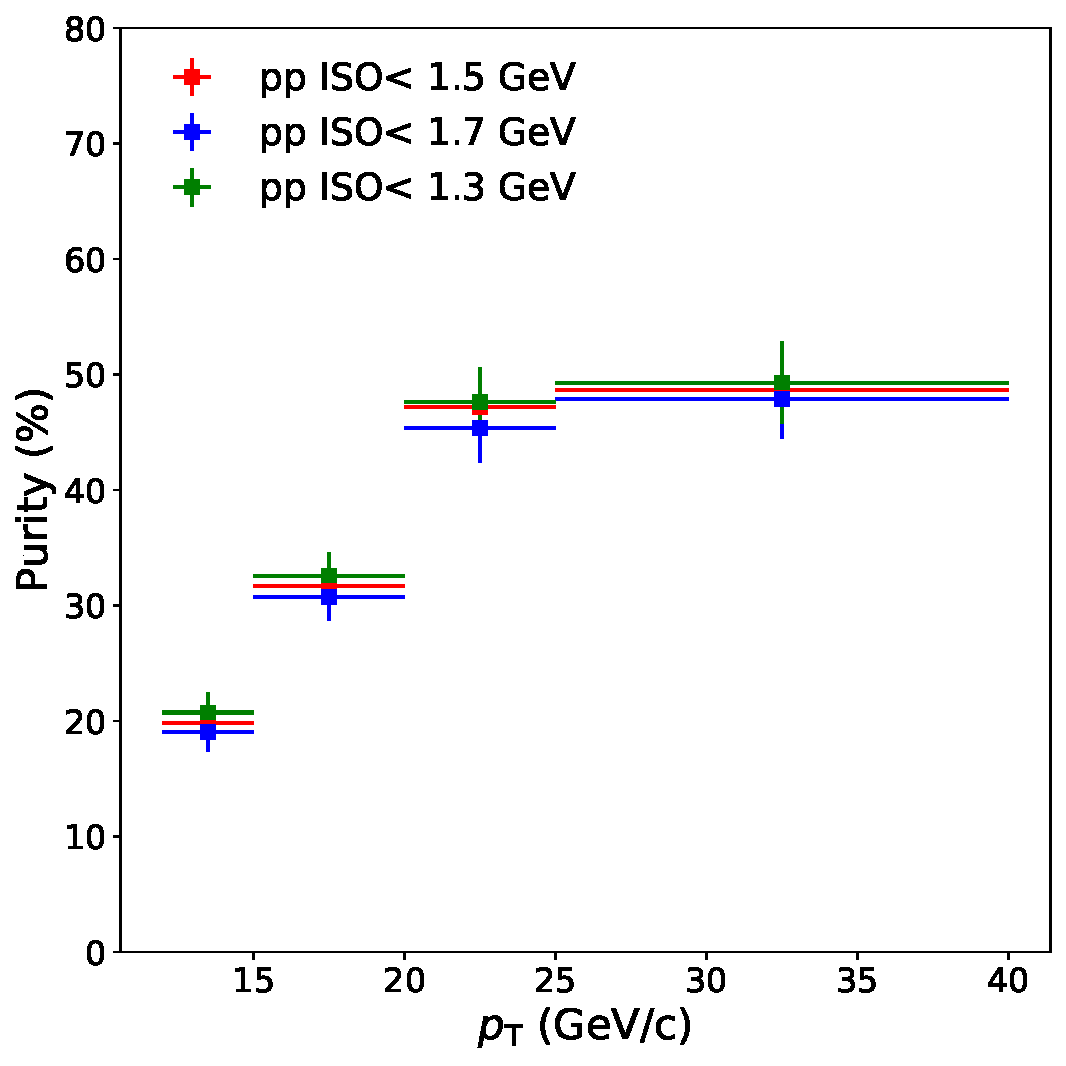
\includegraphics[width=0.495\textwidth]{Checks_Systematics/ppiso.pdf}
	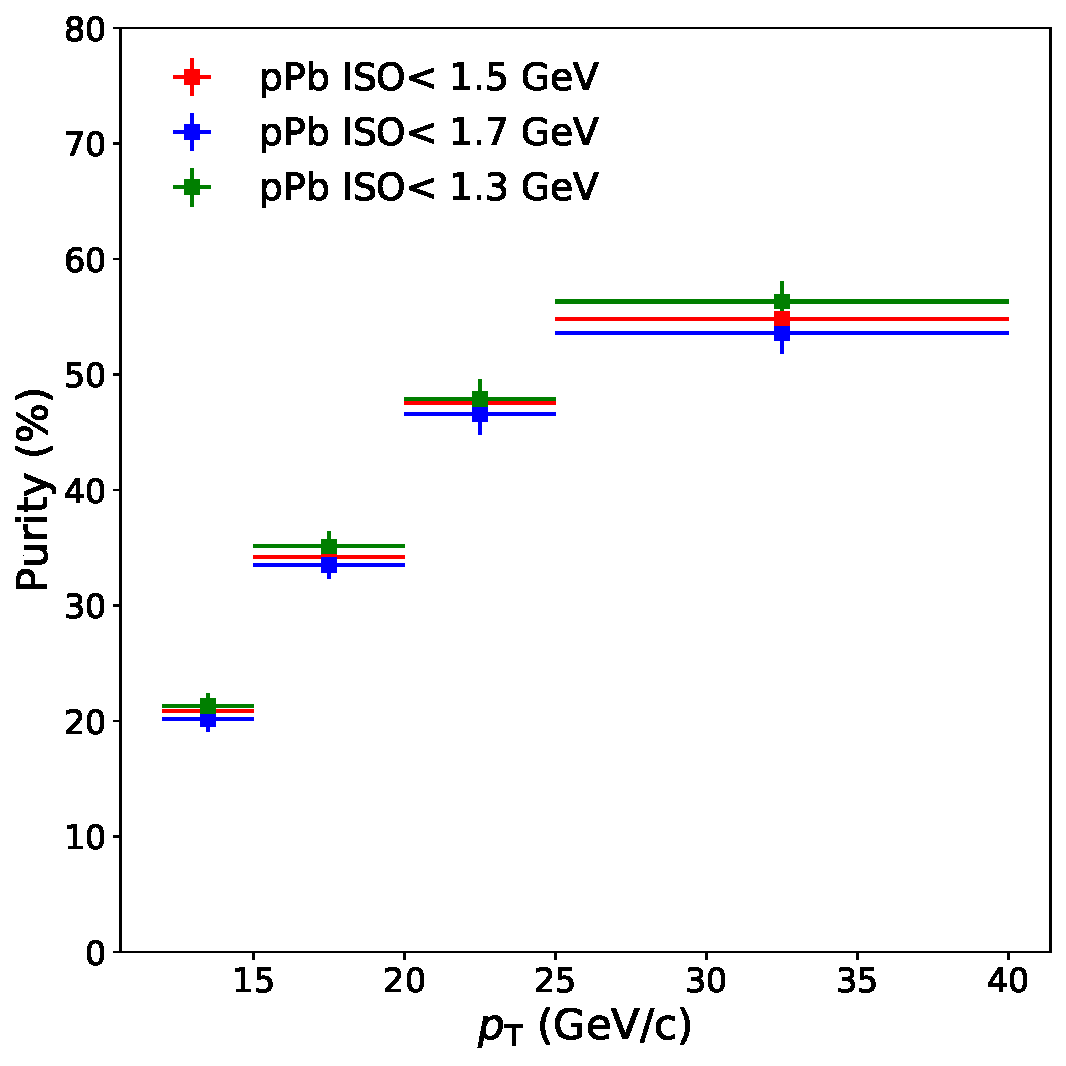
\includegraphics[width=0.495\textwidth]{Checks_Systematics/ppbiso.pdf}
	\caption{Purity measurement with different isolation threshold requirements in pp (left) and \pPb~(right) data.}
	\label{fig:isolationvariation}
\end{figure}




Given that the impact of these cluster variations on the purity measurement is small compared to the estimated systematic uncertainties (described in Section~\ref{sec:puritysystematics}), an additional systematic uncertainty due to cluster selection is not assigned. 

\section{MC-based correction for background template}
\label{sec:MCbasedcorrection}

Figure~\ref{fig:bkgCorrection} shows the weight correction (see Equation~\ref{eq:bkgtemplatecorrection}) applied to the anti-isolation shower-shape distribution, which is obtained from dijet MC simulation. As described in more detail in Section~\ref{sec:purity}, only the shape of this correction is relevant as the normalization is actually fixed in the template fit. The systematic uncertainty associated with this correction is obtained with a double-ratio using data in the background-dominated region ($\lambdasquare>0.4$), as described in more detail in Section~\ref{sec:puritysystematics}. 

\begin{figure}
	\center
	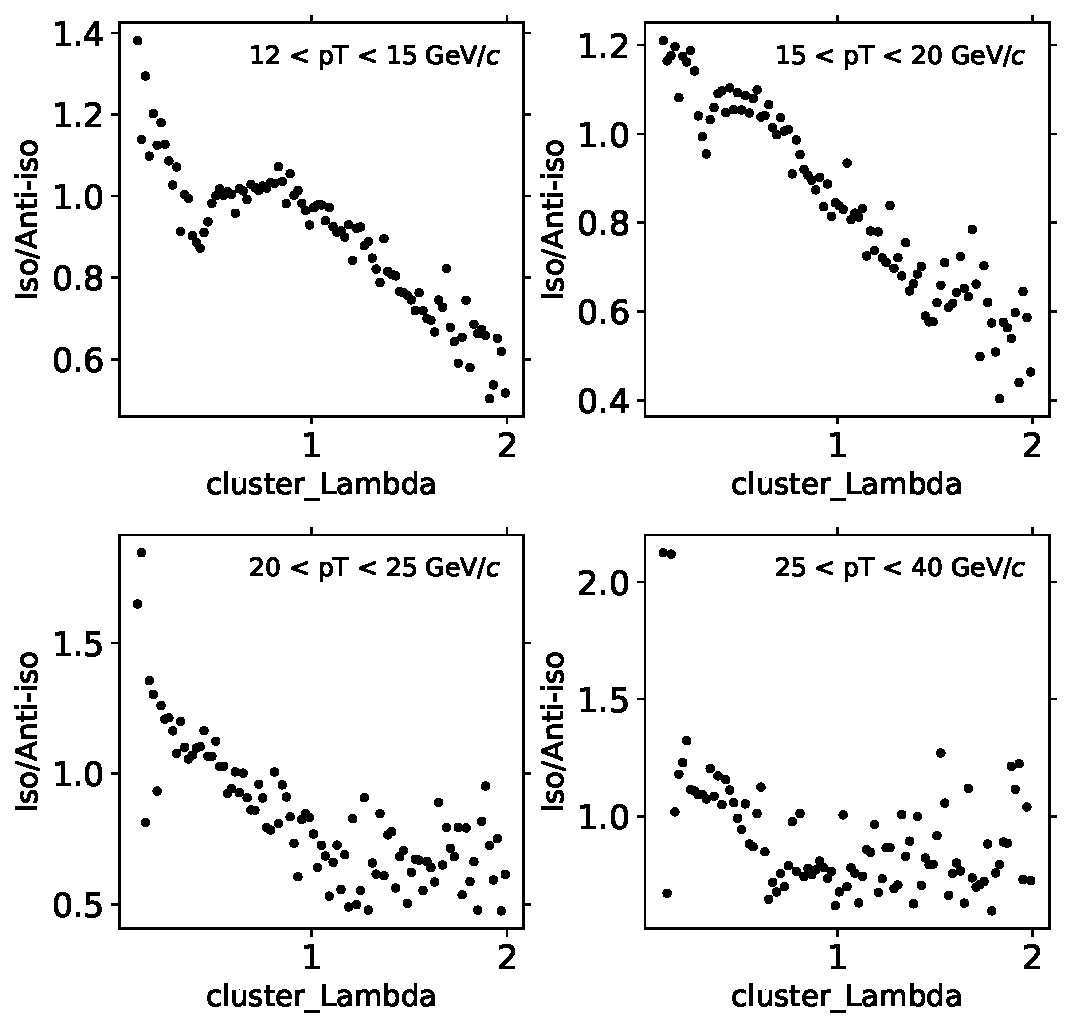
\includegraphics[width=0.76\textwidth]{Checks_Systematics/bkg-template-correction-p-Pb}
	%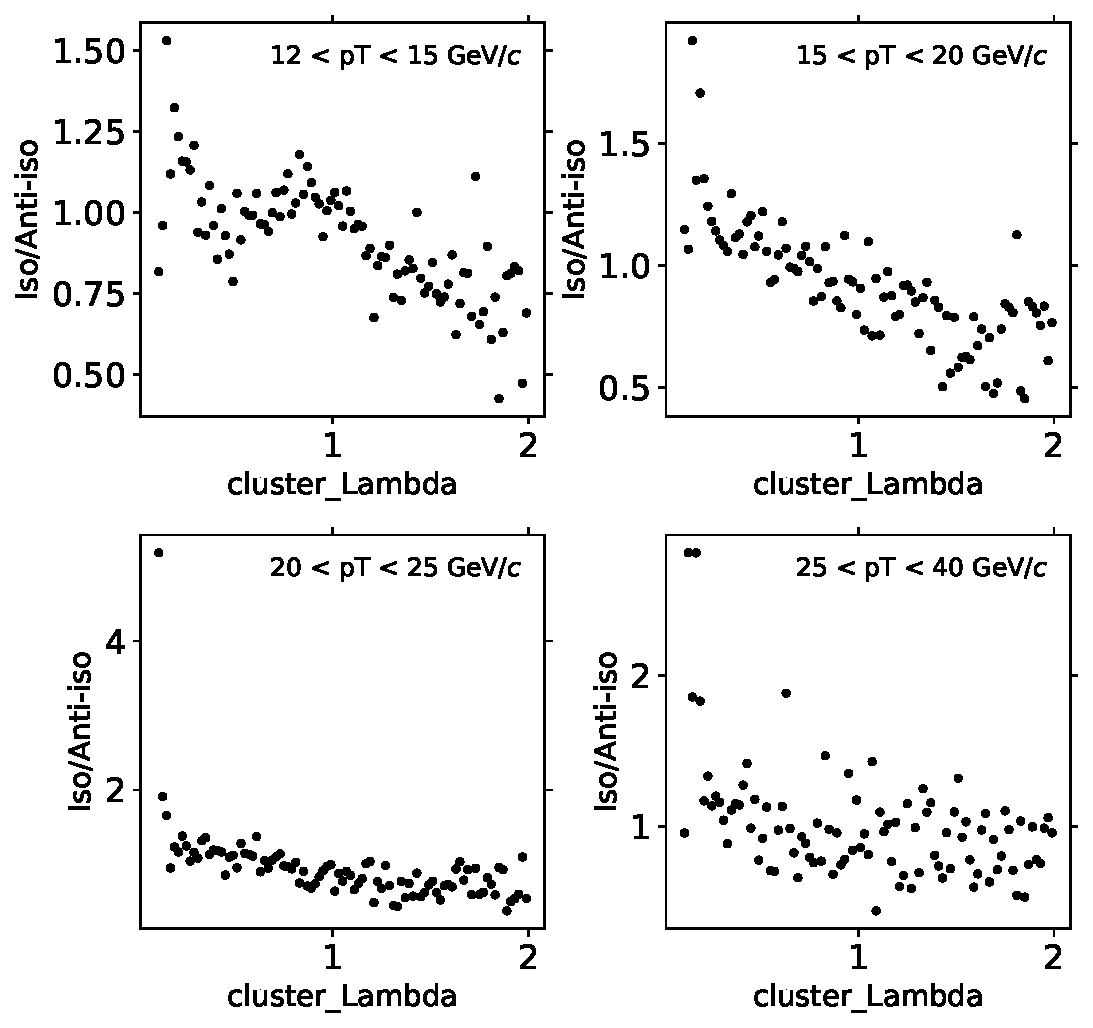
\includegraphics[width=0.495\textwidth]{Checks_Systematics/bkg-template-correction-pp}
	\caption{MC-based correction applied to the background shower-shape template for \pPb~collisions in various $\pt$ ranges.}
	\label{fig:bkgCorrection}
\end{figure}

\section{Checks on Error Function Fits to Purity}
The purity is fit to a 3-parameter error function, shown in Section \ref{purity_err_fit}, in order to capture the quickly rising behavior at low photon-\pt~ and to avoid bin-edge effects. The use of an error function was chosen at it best represents the data as shown in Figure \ref{Fig:Fit_variations}

\begin{figure}
    \centering
    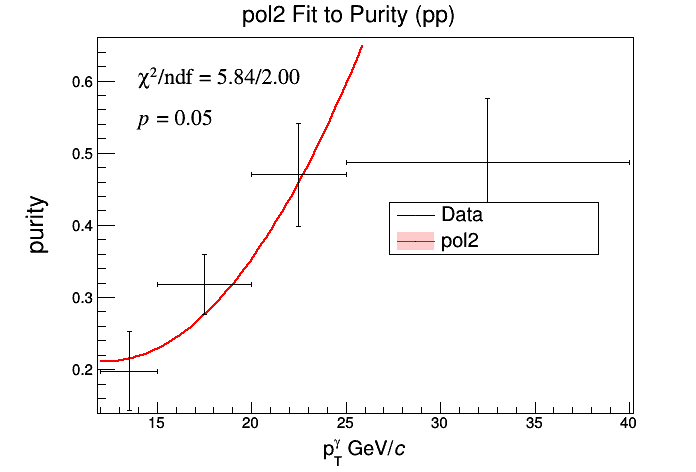
\includegraphics[width=0.495\textwidth]{Checks_Systematics/Pol2}
    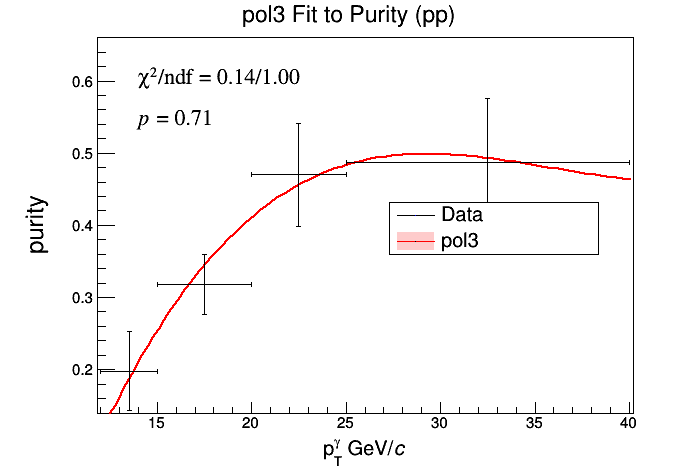
\includegraphics[width=0.495\textwidth]{Checks_Systematics/pol3}
    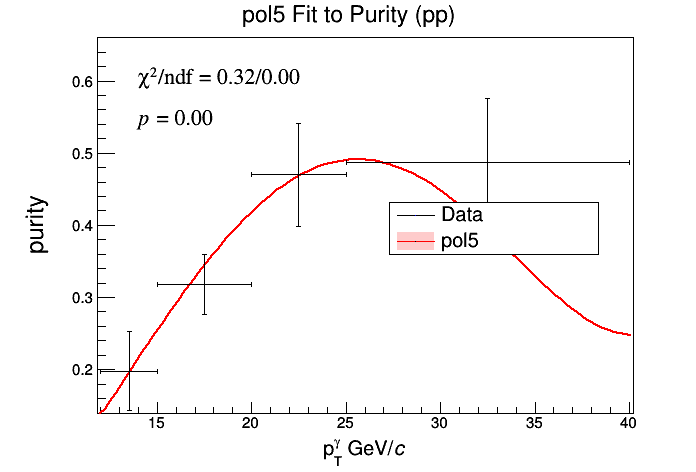
\includegraphics[width=0.495\textwidth]{Checks_Systematics/pol5}
    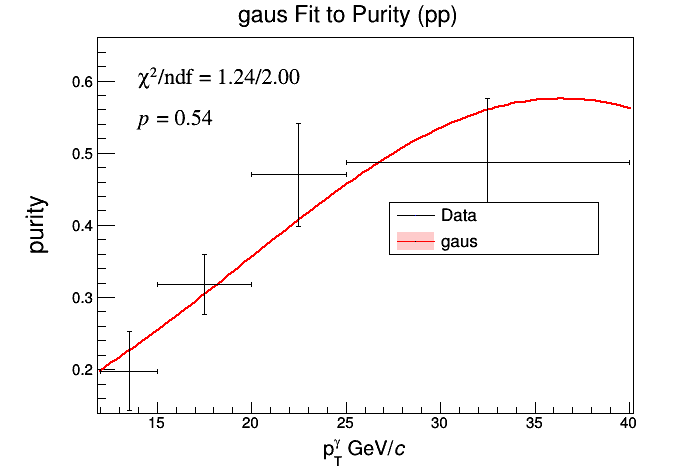
\includegraphics[width=0.495\textwidth]{Checks_Systematics/gauss}
    \includegraphics[width=0.495\textwidth]{Checks_Systematics/EF_Fit}
    \caption{Various functions fit the purity in pp. While there is no simple physics-motivated reason to use the error-function, it was the only function to simultaneously capture the quick rise at low \pt~as well as the plateau at high \pt.}
    \label{Fig:Fit_variations}
\end{figure}

It is important to note that the uncertainty on the fit is not propagated as an uncertainty on correlation analysis. The uncertainty arising from the purity is discussed in detail in Section \ref{sec:puritysystematics}. The fit is used for convenience and enables a cluster-by-cluster weighting when constructing the decay-\gammaiso~ hadron correlation, followed by the correlated subtraction. The error function agrees well within the purity uncertainties, seen in Section \ref{purity_err_fit} as well as in the last panel in Figure~\ref{Fig:Fit_variations}.

Additionally, a check was performed to study the effect that shifting the bin-centers horizontally would have on the fit. A comparison was made between using the linear center of the bins as the bin-center and using the mean \pt~ for the photon-bin (this essentially shifts the bin centers towards lower values of \pt~ due to the quickly falling photon \pt~ spectrum). This comparison is shown for pp and \pPb~ in Figure \ref{Fig:Error_Fit_Mean_Center}.

\begin{figure}
    \centering
    \includegraphics[width=.49\textwidth]{Checks_Systematics/pp_MeanVsBinCenter.png}
    \includegraphics[width=.49\textwidth]{Checks_Systematics/pPb_Compare.png}
    \caption{Comparison of two different bin-centers for used in the purity-error function fit. Blue indicates the fit using the linear center of the bin \pt bin-width. The red represents using the mean \pt for that \gammaiso~ \pt-bin. The left panel shows the comparison for pp, while the right panel shows the comparison for \pPb. The x-axis is the \gammaiso \pt in units of \GeVc. While a small difference is observed, it is well within the uncertainties on the purity, as well as in the the fits' confidence intervals.}
    \label{Fig:Error_Fit_Mean_Center}
\end{figure}

\section{Smearing signal template}
\label{sec:smearingsignaltemplate}
As part of the investigation into evaluating the template fit systematic uncertainty, studies were performed on ''smearing'' of the signal-shape template. That is, for each cluster the measured \lambdasquare~is smeared by multiplying it by some random number drawn from a Gaussian centered at unity with a given standard deviation ''smearing width''.

\begin{figure}
	\center
	\includegraphics[width=0.495\textwidth]{Checks_Systematics/smeared-chi2s-pp-cluster_Lambda-15-20.pdf}
		\includegraphics[width=0.495\textwidth]{Checks_Systematics/smeared-purities-pp-cluster_Lambda-15-20.pdf}
		\caption{Left: Signal template distribution for various smearing widths. Right: purity vs smearing width. The error bar represents the statistical uncertainty, which has been scaled by $\sqrt{\chi^{2}/\mathrm{DOF}}$.}
	\label{fig:smearingSignalShape}
\end{figure}

Figure~\ref{fig:smearingSignalShape} shows the purity obtained for $15<\pt<20$ \GeVc~as a function of smearing width used and the corresponding $\chi^{2}$/DOF. A rather significant deterioration of the $\chi^{2}$ with increasing smearing width is observed, which indicates that smearing beyond $\approx3\%$ is strongly disfavoured by the data. To account for the deterioration of the $\chi^{2}$ that is observed with the smearing, the statistical error of the purity is multiplied by a scaling factor of $\sqrt{\chi^{2}/\mathrm{DOF}}$. A trend of decreasing purity with increasing smearing width is found, but this trend can be accounted for by the artificial worsening of the goodness-of-fit. 


A constant is fit to the purity values vs smearing widths (shown as band in Figure~\ref{fig:smearingSignalShape}). The error on that constant fit and its deviation of its central value from the nominal result (smearing width equal to zero) is below and absolute 1$\%$ difference, which is much smaller than the signal-template uncertainty based on the background-only template fit described in Section~\ref{sec:puritysystematics}. The same conclusion holds for all \pt~ranges in both the pp and \pPb~data.  


\section{Checking sensitivity to $\Delta\varphi$ binning }

Here, the impact of binning on the final correlation functions is quantified. The binning in principle could affect the ZYAM estimate and the shape of the correlation peak. Results are shown with double the number of $\Delta\varphi$ bins. This is done for simplicity in order to be able to integrate the correlation in exactly the same window as reported in the nominal results ($\Delta\varphi>7\pi/8$). The integration window is varied separately from this study. Figure~\ref{fig:dPhivariation} shows the correlation function obtained with double the number of bins as the nominal result. The main conclusion of the study does not change: in every \zt~bin, the pp and \pPb~data are compatible within uncertainties (as quantified in the figure by the $\chi^{2}$~and corresponding p-value), and the \textsc{Pythia8} describes the data within uncertainties. 

\begin{sidewaysfigure}
\label{fig:dPhivariation}
\centering
\includegraphics[width = 0.24 \textwidth]{G-H_New/16_dPhi/Cs_Final_Indv_pT_0_zT_0.pdf}
\includegraphics[width = 0.24 \textwidth]{G-H_New/16_dPhi/Cs_Final_Indv_pT_0_zT_1.pdf}
\includegraphics[width = 0.24 \textwidth]{G-H_New/16_dPhi/Cs_Final_Indv_pT_0_zT_2.pdf}
\includegraphics[width = 0.24 \textwidth]{G-H_New/16_dPhi/Cs_Final_Indv_pT_0_zT_3.pdf}
\includegraphics[width = 0.24 \textwidth]{G-H_New/16_dPhi/Cs_Final_Indv_pT_0_zT_4.pdf}
\includegraphics[width = 0.24 \textwidth]{G-H_New/16_dPhi/Cs_Final_Indv_pT_0_zT_5.pdf}
\includegraphics[width = 0.24 \textwidth]{G-H_New/16_dPhi/Cs_Final_Indv_pT_0_zT_6.pdf}
\includegraphics[width = 0.24 \textwidth]{G-H_New/16_dPhi/Cs_Final_Indv_pT_0_zT_6.pdf}
\caption{Fully-corrected $\gammaiso$--hadron correlation function pp (red) and \pPb~(blue) data. The purple band represents the uncertainty from the underlying event estimate in pp and \pPb. The error bars represent statistical uncertainty only. The green line is the \gammaiso--hadron correlation function obtained with \textsc{PYTHIA 8.2}. The key difference with the nominal results shown in Section~\ref{sec:results} the number of $\Delta\varphi$ bins is doubled.}
\end{sidewaysfigure}

%\begin{figure}
%\centering
%\includegraphics[width = 0.49 \textwidth]{G-H_New/16_dPhi/Ratio_FF_Averages_Phi_Rebinning}
%\caption{Comparison of ratio of fragmentation functions with different $\Delta\varphi$ binning.}
%\label{fig:dPhiRatio}
%\end{figure}

\section{Checking Sensitivity to Beam Flip}
Figure~\ref{fig:Cs_Beam_Flip} shows results for 13de and 13f periods. They differ in the beam configuration and have roughly similar integrated luminosity. No significant difference is observed. 

\begin{figure}
\centering
\includegraphics[width = 0.9 \textwidth]{G-H_New/Cs_Averages_p-Pb_Beam_Flip.pdf}
\caption{Comparison of final correlations functions for p--Pb (red) and Pb--p (blue) collisions.}
\label{fig:Cs_Beam_Flip}
\end{figure}



\section{Correlations including $\Delta\varphi=0$ }
Figure~\ref{fig:CorrelationFinal_downtozero} shows the correlation results down to 0 radians. The first bin is contained within the isolation requirement and therefore is biased, which is why is not reported in the main results. 

\begin{sidewaysfigure}
\centering
\includegraphics[width = 0.24 \textwidth]{G-H_New/dPhi_to_0/Cs_Final_Indv_pT_0_zT_0.pdf}
\includegraphics[width = 0.24 \textwidth]{G-H_New/dPhi_to_0/Cs_Final_Indv_pT_0_zT_1.pdf}
\includegraphics[width = 0.24 \textwidth]{G-H_New/dPhi_to_0/Cs_Final_Indv_pT_0_zT_2.pdf}
\includegraphics[width = 0.24 \textwidth]{G-H_New/dPhi_to_0/Cs_Final_Indv_pT_0_zT_3.pdf}
\includegraphics[width = 0.24 \textwidth]{G-H_New/dPhi_to_0/Cs_Final_Indv_pT_0_zT_4.pdf}
\includegraphics[width = 0.24 \textwidth]{G-H_New/dPhi_to_0/Cs_Final_Indv_pT_0_zT_5.pdf}
\includegraphics[width = 0.24 \textwidth]{G-H_New/dPhi_to_0/Cs_Final_Indv_pT_0_zT_6.pdf}
\includegraphics[width = 0.24 \textwidth]{G-H_New/dPhi_to_0/Cs_Final_Indv_pT_0_zT_7.pdf}
\caption{Fully-corrected $\gammaiso$--hadron correlation function pp (red) and \pPb~(blue) data. Identical to Figure \ref{fig:CorrelationFinal} with the exception that the correlation functions down to $\Delta\varphi$=0 are shown.}
\label{fig:CorrelationFinal_downtozero}
\end{sidewaysfigure}

%\begin{sidewaysfigure}
%\label{fig:dPhivariation}
%\centering
%\includegraphics[width = 0.24 %\textwidth]{G-H_New/dPhi_to_0/Cs_Final_Indv_pT_0_zT_0.pdf}
%\includegraphics[width = 0.24 %\textwidth]{G-H_New/dPhi_to_0/Cs_Final_Indv_pT_0_zT_1.pdf}
%\includegraphics[width = 0.24 %\textwidth]{G-H_New/dPhi_to_0/Cs_Final_Indv_pT_0_zT_2.pdf}
%\includegraphics[width = 0.24 %\textwidth]{G-H_New/dPhi_to_0/Cs_Final_Indv_pT_0_zT_3.pdf}
%\includegraphics[width = 0.24 \textwidth]{G-H_New/dPhi_to_0/Cs_Final_Indv_pT_0_zT_4.pdf}
%\includegraphics[width = 0.24 \textwidth]{G-H_New/dPhi_to_0/Cs_Final_Indv_pT_0_zT_5.pdf}
%\includegraphics[width = 0.24 %\textwidth]{G-H_New/dPhi_to_0/Cs_Final_Indv_pT_0_zT_6.pdf}
%\includegraphics[width = 0.24 %\textwidth]{G-H_New/dPhi_to_0/Cs_Final_Indv_pT_0_zT_7.pdf}
%\caption{Fully-corrected $\gammaiso$--hadron correlation function pp (red) and \pPb~(blue) data. The purple band represents the uncertainty from the underlying event estimate in pp and \pPb. The error bars represent statistical uncertainty only. The green line is the \gammaiso--hadron correlation function obtained with \textsc{PYTHIA 8.2}. This difference with the nominal results shown in Section~\ref{sec:results} is that here we double the number of $\Delta\varphi$ bins.}
%\end{sidewaysfigure}

\section{Comparing ITS only tracking to ITS+TPC Tracking}

This section compares results obtained using hybrid (ITS + TPC) tracks in the triggered 13def data (\pPb). Other than the change in the appropriate tracking corrections, the analysis chain is identical to the one that uses the ITS-only tracking. Figure \ref{fig:TPC_CorrelationFinal} shows the correlation functions for \pPb~that uses hybrid tracks and pp which only uses ITS tracks (the TPC was not read out during the 17q data taking).

\begin{sidewaysfigure}
\centering
\includegraphics[width = 0.24 \textwidth]{G-H_New/TPC_Tracks/Cs_Final_Indv_pT_0_zT_0.pdf}
\includegraphics[width = 0.24 \textwidth]{G-H_New/TPC_Tracks/Cs_Final_Indv_pT_0_zT_1.pdf}
\includegraphics[width = 0.24 \textwidth]{G-H_New/TPC_Tracks/Cs_Final_Indv_pT_0_zT_2.pdf}
\includegraphics[width = 0.24 \textwidth]{G-H_New/TPC_Tracks/Cs_Final_Indv_pT_0_zT_3.pdf}
\includegraphics[width = 0.24 \textwidth]{G-H_New/TPC_Tracks/Cs_Final_Indv_pT_0_zT_4.pdf}
\includegraphics[width = 0.24 \textwidth]{G-H_New/TPC_Tracks/Cs_Final_Indv_pT_0_zT_5.pdf}
\includegraphics[width = 0.24 \textwidth]{G-H_New/TPC_Tracks/Cs_Final_Indv_pT_0_zT_6.pdf}
\includegraphics[width = 0.24 \textwidth]{G-H_New/TPC_Tracks/Cs_Final_Indv_pT_0_zT_7.pdf}
\caption{Fully-corrected $\gammaiso$--hadron correlation function in pp using ITS only tracks (red) and \pPb~ using hybrid tracks (blue).}
\label{fig:TPC_CorrelationFinal}
\end{sidewaysfigure}

\begin{figure}
\centering
\includegraphics[width = 0.49 \textwidth]{G-H_New/TPC_Tracks/Final_FFunction_and_Ratio.pdf}
\includegraphics[width = 0.49 \textwidth]{G-H_New/TPC_Tracks/TPC_Compare_Final_FFunction_and_Ratio.pdf}
\caption{Left: Comparison of final correlations functions for \pPb~Hybrid tracks (blue) and pp ITS only tracks (red). Right: Comparison of final correlations functions for \pPb~Hybrid tracks (red) and \pPb~ITS only tracks (blue).}
\label{fig:TPC_FF}
\end{figure}


Figure \ref{fig:TPC_FF} Shows the fragmentation studies in \pPb~data with ITS only tracks and Hybrid tracks. It can be seen in the ratio of ITS Only/Hybrid that the hybrid tracks have a significantly lower yield at high \zt, which roughly corresponds to tracks with high \pt. This is unsurprising as there are issues with TPC charge distortions that have been documented at length [https://alice.its.cern.ch/jira/browse/ATO-351].

\section{Checking sensitivity to $\zt$ binning}
This section looks into varying the number of \zt bins. Figure \ref{fig:FF_zT_Rebin} shows the resulting fragmentation function in 6 $zt$ bins. 


\begin{figure}
\centering
\includegraphics[width=0.49\textwidth]{G-H_New/zT_Rebin_6_006zT06zTITSSub/Final_FFunction_and_Ratio.pdf}
\label{fig:FF_zT_Rebin}
\caption{Results with variation of numbers of \zt~bins. }
\end{figure}


%\FloatBarrier

\section{Checking sensitivity to pile up cut in pp}
A stringent pile up cut is applied to the pp dataset. Figure \ref{fig:Correlation_pileup} shows the correlation functions in 6 $\zt$ bins to compensate for the loss of statistics in pp after applying the cut.

\begin{sidewaysfigure}
\centering
\includegraphics[width = 0.32 \textwidth]{G-H_New/zT_Rebin_6_006zT06zTpileCut/Cs_Final_Indv_pT_0_zT_0.pdf}
\includegraphics[width = 0.32 \textwidth]{G-H_New/zT_Rebin_6_006zT06zTpileCut/Cs_Final_Indv_pT_0_zT_1.pdf}
\includegraphics[width = 0.32 \textwidth]{G-H_New/zT_Rebin_6_006zT06zTpileCut/Cs_Final_Indv_pT_0_zT_2.pdf}
\includegraphics[width = 0.32 \textwidth]{G-H_New/zT_Rebin_6_006zT06zTpileCut/Cs_Final_Indv_pT_0_zT_3.pdf}
\includegraphics[width = 0.32 \textwidth]{G-H_New/zT_Rebin_6_006zT06zTpileCut/Cs_Final_Indv_pT_0_zT_4.pdf}
\includegraphics[width = 0.32 \textwidth]{G-H_New/zT_Rebin_6_006zT06zTpileCut/Cs_Final_Indv_pT_0_zT_5.pdf}

\caption{Fully-corrected $\gammaiso$--hadron correlation function in pp (red) and \pPb~(blue) data with the pile up cut in pp only. The correlations have been rebinned to 6 \zt bins to compensate for the loss in statistics after applying the cut.}
\label{fig:Correlation_pileup}
\end{sidewaysfigure}

\begin{figure}
\centering
\includegraphics[width=0.59\textwidth]{G-H_New/zT_Rebin_6_006zT06zTpileCut/Final_FFunction_and_Ratio.pdf}
\caption{The fragmentation functions with the pile up cut applied to pp, resulting from the correlation functions shown in Fig.~\ref{fig:Correlation_pileup}.}
\label{fig:FF_pileup}
\end{figure}


Figure \ref{fig:FF_pileup} shows the resulting fragmentation function in 6 $zt$ bins with the pile up cut applied to the pp data. The figure shows no significant change as a result of this cut.


\section{Checking Maximum Track $\pt$ Cut}
This section explores the effect of varying the maximum $\pt$ cut on the final away-side yields in pp and \pPb and the effect of this variation on the final ratio is shown.

\begin{figure}
\includegraphics[width=0.49\textwidth]{G-H_New/FF_Averages_Max_pT_pp.pdf}
\includegraphics[width=0.49\textwidth,height=0.42\textwidth]{G-H_New/Ratio_FF_Averages_Max_pT.pdf}
\caption{Left: The away side yields in pp with a maximum $p_\mathrm{T}^\mathrm{Track}$ cut of 10, 8, and 6 GeV/$c$. Right: The Ratio of \pPb~to pp with a maximum $p_\mathrm{T}^\mathrm{Track}$ cut of 10, 8, and 6 GeV/$c$}
\label{fig:FF_pT_Max_pp}
\end{figure}


% \section{Purity result with newly reconstructed data}

% Figure~\ref{newpurity} shows the purity measurement obtained with the newly reconstructed 13f data. The measurements are compatible within statistical variations. 

% \begin{figure}
% \centering
% \includegraphics[width=0.5\textwidth]{Purity/purities13ffinal.pdf}
% \caption{Nominal results for purity and purity measured with the newly reconstructed 13f runs.}
% \label{newpurity}
% \end{figure}


\section{Sensitivity to $\chi^2/\mathrm{ITS}_{clus}$ in p-Pb}
The effect of the $\chi^2/\mathrm{ITS}_{clus}$ cut on the tracking efficiency, fake rate, and bin migration is studied to select the most effective $\chi^2/\mathrm{ITS}_{clus}$ maximum limit. Four values have been tested: $\chi^2/\mathrm{ITS}_{clus} =$ 1, 2, 3, and 36. The following figures~\ref{fig:chi2_eff}, ~\ref{fig:chi2_fr}, ~\ref{fig:chi2_bm}, and ~\ref{fig:chi2_w} show the effect of $\chi^2/\mathrm{ITS}_{clus}$ cuts on the efficiency, fake rate, bin migration, and track correction weight. The weight is calculated from the efficiency, fake rate, and bin migration using equation~\ref{eq:track_weight}. The efficiency seems to be similar for all cut variation except for $\chi^2/\mathrm{ITS}_{clus}$ < 1, where it is lower by 5\%. However, the fake rate and bin migration effects are improved as the cut is tightened. It is to note that regardless of the threshold for the $\chi^2/\mathrm{ITS}_{clus}$ cut, as long as identical cuts are applied to both the Monte Carlo and the data sets used in the section~\ref{sec:tracking}, the fine agreement with published data is always present.

\begin{figure}[h]
    \centering
    \includegraphics[width=0.49\textwidth]{Checks_Systematics/ITSchi2_study_efficiency.pdf}
        \includegraphics[width=0.49\textwidth]{Checks_Systematics/ITSchi2_study_fakerate.pdf}
    \caption{Left: The efficiency comparison for the various $\chi^2/\mathrm{ITS}_{clus}$ cuts. Right: The fake rate comparison for the various $\chi^2/\mathrm{ITS}_{clus}$ cuts}
    \label{fig:chi2_eff}
\end{figure}

Additionally, figure~\ref{fig:chi2SpectraComparison} shows the effect of changing the $\chi^2/ITS_{clus}$ from $\chi^2/ITS_{clus} < 36$ to $\chi^2/ITS_{clus} < 3$ on the track \pt spectra as the ratio of $\chi^2/ITS_{clus} <3$ and $\chi^2/ITS_{clus} < 36$. From the top two plots, one can see that the change in the cut does not affect the \pt spectra as the raito is consistent with unity within 5\% up 8 GeV/ as along as the appropriate Monte Carlo anchored to the data is used. However, the bottom plots, uses LHC13def, but corrects using the 13b2 Monte Carlo, and divergence from unity shows the instability of the $\chi^2/ITS_{clus}$ cut. Thus, the 13b2 Monte Carlo is not used in place of using the 17g6a1 simulation to correct the 13def data set.
\begin{figure}[h]
\center
\includegraphics[width=0.33\textwidth]{Checks_Systematics/ITSchi2_study_ptSpectra_ratio_MBMB.pdf}
\includegraphics[width=0.33\textwidth]{Checks_Systematics/ITSchi2_study_ptSpectra_ratio_MBGJ.pdf}
\includegraphics[width=0.33\textwidth]{Checks_Systematics/ITSchi2_study_ptSpectra_ratio_GJGJ.pdf}
\caption{The changes in the tracking spectra with respect to the $\chi^2/ITS_{clus}$ cut. The top left is the 13b data corrected using 13b2 Monte Carlo. The top right is 13def data corrected using 17g6a1 Monte Carlo. And the bottom plot is 13def data corrected using 13b2 Monte Carlo.}
\label{fig:chi2SpectraComparison}
\end{figure}

Finally, the efficiency, fake rate, bin migration and the weights are compared between ITS-only tracking in p-Pb and pp, and TPC+ITS tracking in p-Pb using 17g6a1 MC dataset. All the TPC+ITS and ITS-only tracking are comparable within uncertainties, while the ITS-only pp and p-Pb follow similar shapes. This result agrees with acceptations and trend demonstrated in section~\ref{sec:tracking}. The key difference is that in section~\ref{sec:tracking} all the figures are produced using 13b2, the minimum bias Monte Carlo, while in the case for figure~\ref{fig:TPCITSpp_pPbCompare}, 17g6a1, the gamma-jet Monte Carlo is used. 
\begin{figure}[h]
\center
\includegraphics[width=0.46\textwidth]{Checks_Systematics/ITSchi2_study_efficiency.pdf}
\includegraphics[width=0.46\textwidth]{Checks_Systematics/ITSchi2_study_fakerate.pdf}
\includegraphics[width=0.46\textwidth]{Checks_Systematics/ITSchi2_study_binMigration.pdf}
\includegraphics[width=0.46\textwidth]{Checks_Systematics/ITSchi2_study_weight.pdf}
\caption{The comparison of efficiency (top left), fake rate (top right), bin migration (bottom left), and weights (bottom right) between ITS-only tracking for p-Pb and pp, as well as TPC+ITS tracking for p-Pb using the 17g6a1 gamma-jet Monte Carlo.}
\label{fig:TPCITSpp_pPbCompare}

\end{figure}

